\documentclass[man,floatsintext]{apa7}
\usepackage[american]{babel}
\usepackage[utf8]{inputenc}
\usepackage{csquotes}
\usepackage{amsmath,amssymb}
\usepackage{booktabs}
\usepackage{graphicx}
\usepackage{float}
\usepackage{multirow}
\usepackage{array}
\usepackage{tabularx}
\usepackage{hyperref}
\usepackage{threeparttable}
\usepackage{longtable}
\usepackage{pdflscape}
\usepackage{makecell}
\usepackage{placeins}

% APA 7 requires Times New Roman or similar serif font
\usepackage{mathptmx}

% APA biblatex setup (matches the main manuscript)
\usepackage[style=apa,backend=biber,natbib=true,sorting=nyt]{biblatex}
\DeclareLanguageMapping{american}{american-apa}
\addbibresource{references.bib}

% Fill pages by stretching glue rather than leaving short pages with
% blank space at the bottom. This is the LaTeX default for two-sided
% documents and is preferable here because the supplementary contains
% many figures and tables that would otherwise leave large white spaces.
\flushbottom

% Relax LaTeX's float-placement constraints. The supplementary is
% float-heavy (many large tables and figures relative to text), so the
% default thresholds (which assume a text-heavy paper) cause floats to
% be deferred and leave white space at the bottom of preceding pages.
% These settings allow floats to occupy more of each page and float-only
% pages to be less full, which lets the document pack content tightly.
\renewcommand{\topfraction}{0.92}
\renewcommand{\bottomfraction}{0.88}
\renewcommand{\textfraction}{0.05}
\renewcommand{\floatpagefraction}{0.7}
\renewcommand{\dbltopfraction}{0.92}
\renewcommand{\dblfloatpagefraction}{0.7}
\setcounter{topnumber}{4}
\setcounter{bottomnumber}{2}
\setcounter{totalnumber}{6}
\setcounter{dbltopnumber}{4}

% Placeholder image for figures not yet available
\newsavebox{\placeholderbox}
\savebox{\placeholderbox}{%
  \fbox{\parbox[c][6cm][c]{0.9\textwidth}{%
    \centering\large\sffamily [Figure placeholder --- insert image here]%
  }}%
}

\title{Supplementary Materials:\\The Impact of Complexity on Risky Choices: An Evidence Accumulation Account}
\shorttitle{Supplementary Materials}

\author{
Maohua Nie\textsuperscript{1}, J\"org Rieskamp\textsuperscript{1}, Sebastian Olschewski\textsuperscript{1,2}
}

\affiliation{
\textsuperscript{1}Department of Psychology, University of Basel, Switzerland\\
\textsuperscript{2}Warwick Business School, University of Warwick, UK
}

\authornote{
Correspondence concerning this article should be addressed to Maohua Nie, Department of Psychology, University of Basel, Switzerland.\\
Email: \texttt{niemaohua@gmail.com}
}

\begin{document}
\maketitle

\setcounter{section}{0}
\renewcommand{\thesection}{S\arabic{section}}
\renewcommand{\thetable}{S\arabic{table}}
\renewcommand{\thefigure}{S\arabic{figure}}
\renewcommand{\theequation}{S\arabic{equation}}

This document collects the supplementary methods, analyses, and results referenced in the main text---participant exclusions, the hierarchical Bayesian estimation procedure, convergence and recovery diagnostics, the CPT-based robustness analyses, response-time distribution fits, the race-model diagnostic, and the exploratory cognitive-ability analyses. The sections are listed below.

\setcounter{tocdepth}{2}
{\hypersetup{linkcolor=black}\tableofcontents}
\clearpage

%% ============================================================================
\section{Participants and Exclusions}
\label{sec:exclusions}
%% ============================================================================

\subsection{Recruitment and Sample Size}

For each study we set a minimum target of 125 participants (the power justification is given in the main text) and recruited 150 on Prolific to allow for exclusions. In Studies 1 and 2, the data of 2 and 3 participants, respectively, were lost during transfer from Prolific to the JATOS server: these participants completed the experiment and were compensated, but their responses were never recorded. Because they had already been paid from the pre-budgeted 150 slots, recruitment was not topped up. The raw (pre-exclusion) samples with recorded data were therefore $N = 148$ (Study 1), $N = 147$ (Study 2), and $N = 150$ (Study 3).

\subsection{Exclusion Criteria}

We applied the same preregistered exclusion pipeline in every study, in the following order:
\begin{enumerate}
    \item \textbf{Comprehension.} Participants who required more than the allowed number of attempts to answer the four comprehension questions correctly were excluded (more than 8 attempts in Studies 1 and 2; more than 6 in Study 3).
    \item \textbf{Response-time bounds.} Trials with a response time below 1\,s or above 30\,s were removed; the 1\,s lower bound is why the analysed response times have a 1\,s floor.
    \item \textbf{Response-time outliers.} Within each participant and choice category, trials whose response time fell outside the median $\pm\,3$ SD were removed.
    \item \textbf{Excessive trial loss.} Participants who lost more than 50\% of their trials to the response-time screens (criteria 2--3) were excluded.
\end{enumerate}

\subsection{Resulting Samples}

Table~\ref{tab:exclusions} summarises the samples. The final analysed samples were 137, 138, and 132 participants for Studies 1, 2, and 3. The raw data, the cleaning scripts implementing these criteria, and per-participant exclusion records are available in the online repository (see the \nameref{sec:software} section).

\begin{table}[!htbp]
\centering
\begin{threeparttable}
\caption{Participant Recruitment and Exclusions by Study}
\label{tab:exclusions}
\begin{tabular}{llrrrr}
\toprule
\textbf{Study} & \textbf{Complexity type} & \textbf{Raw $N$}\textsuperscript{a} & \textbf{Comprehension} & \textbf{$>$50\% trials} & \textbf{Final $N$} \\
\midrule
Study 1 & Lottery complexity     & 148 & 1 & 10 & 137 \\
Study 2 & Outcome complexity     & 147 & 1 & 8  & 138 \\
Study 3 & Probability complexity & 150 & 8 & 10 & 132 \\
\bottomrule
\end{tabular}
\begin{tablenotes}[flushleft]
\small
\item \textit{Note.} ``Comprehension'' = participants excluded for exceeding the allowed comprehension-question attempts; ``$>$50\% trials'' = participants excluded for losing more than half of their trials to the response-time screens. Trial-level response-time screening was applied before the participant-level $>$50\% rule.
\item \textsuperscript{a} 150 participants were recruited and paid in each study; the raw $N$ is lower for Studies 1 and 2 because 2 and 3 participants' data, respectively, were lost in the Prolific-to-JATOS transfer.
\end{tablenotes}
\end{threeparttable}
\end{table}

%% ============================================================================
\section{Prior Specifications}
\label{sec:priors}
%% ============================================================================

As noted in the main text, all models were estimated using a hierarchical Bayesian framework with a non-centred parameterisation. Here we report the complete prior distributions for all group-level parameters. Priors were chosen to be weakly informative: broad enough to encompass a wide range of plausible values while providing sufficient regularisation to avoid divergent sampling behaviour.

For parameters constrained to be positive (the signal-to-noise ratio $\theta$, the decision threshold $\alpha$, and the non-decision time $T_0$), we used the $\log(1+\exp(\cdot))$ transform: $x_{\text{eff}} = \log(1 + e^{x_{\text{raw}}})$, where $x_{\text{raw}}$ is the unconstrained parameter estimated on the real line. For the starting point $z$ in CS models, we used the probit transform: $z = \Phi(z_{\text{raw}})$. The prior centres for transformed parameters were chosen so that the implied prior predictive distribution of the effective parameter covered psychologically plausible ranges.

\begin{table}[!htbp]
\centering
\begin{threeparttable}
\caption{Prior Distributions for Group-Level Parameters: MVS Models}
\label{tab:priors_mvs}
\begin{tabular}{llllc}
\toprule
\textbf{Parameter} & \textbf{Symbol} & \textbf{Transform} & \textbf{Prior on $\mu_k$} & \textbf{Implied centre} \\
\midrule
Risk preference (SDD weight)  & $\beta$      & none                  & $N(0, 3)$   & 0 \\
Signal-to-noise ratio         & $\theta$     & $\log(1{+}e^{\cdot})$ & $N(-2, 3)$  & 0.13 \\
Decision threshold            & $\alpha$     & $\log(1{+}e^{\cdot})$ & $N(5, 3)$   & 5.0 \\
Non-decision time             & $T_0$        & $\log(1{+}e^{\cdot})$ & $N(-1, 1)$ & 0.31\,s \\
Skewness preference (SkewD weight) & $\eta$ & none                  & $N(0, 3)$   & 0 \\
Starting point\textsuperscript{a}  & $z$    & $\Phi(\cdot)$         & $N(0, 1)$   & 0.5 \\
Drift rate adjustment\textsuperscript{a} & $\zeta$ & none           & $N(0, 5)$   & 0 \\
All shift parameters          & $\Delta_x$   & none                  & $N(0, 3)$   & 0 \\
Group-level SDs               & $\sigma_k$   & ---                   & Exp$(1)$    & --- \\
Correlation matrix            & $\mathbf{\Omega}$ & Cholesky         & LKJ$(1)$    & --- \\
Individual deviations         & $z_{k,l}$    & ---                   & $N(0, 1)$   & --- \\
\bottomrule
\end{tabular}
\begin{tablenotes}[flushleft]
\small
\item \textit{Note.} $N(\mu, \sigma)$ = normal distribution; Exp$(\lambda)$ = exponential; LKJ$(\eta)$ = Lewandowski--Kurowicka--Joe prior. ``Implied centre'' gives the approximate effective-scale value after transformation.
\item \textsuperscript{a} Included only in CS models.
\end{tablenotes}
\end{threeparttable}
\end{table}

\begin{table}[!htbp]
\centering
\begin{threeparttable}
\caption{Prior Distributions for Group-Level Parameters: CPT-Based Models}
\label{tab:priors_cpt}
\begin{tabular}{llllc}
\toprule
\textbf{Parameter} & \textbf{Symbol} & \textbf{Transform} & \textbf{Prior on $\mu_k$} & \textbf{Implied centre} \\
\midrule
Utility curvature             & $\beta_{\text{CPT}}$ & $\log(1{+}e^{\cdot})$ & $N(0.54, 3)$ & 1.0 \\
Signal-to-noise ratio         & $\theta$     & $\log(1{+}e^{\cdot})$ & $N(-1, 3)$   & 0.31 \\
Decision threshold            & $\alpha$     & $\log(1{+}e^{\cdot})$ & $N(5, 3)$    & 5.0 \\
Non-decision time             & $T_0$        & $\log(1{+}e^{\cdot})$ & $N(-1, 1)$   & 0.31\,s \\
Probability weighting         & $\gamma$     & $\log(1{+}e^{\cdot})$ & $N(0.54, 3)$ & 1.0 \\
Starting point\textsuperscript{a}  & $z$    & $\Phi(\cdot)$         & $N(0, 3)$    & 0.5 \\
Drift rate adjustment\textsuperscript{a} & $\zeta$ & none           & $N(0, 3)$    & 0 \\
All shift parameters          & $\Delta_x$   & none                  & $N(0, 3)$    & 0 \\
Group-level SDs               & $\sigma_k$   & ---                   & Exp$(1)$     & --- \\
Correlation matrix            & $\mathbf{\Omega}$ & Cholesky         & LKJ$(1)$     & --- \\
Individual deviations         & $z_{k,l}$    & ---                   & $N(0, 1)$    & --- \\
\bottomrule
\end{tabular}
\begin{tablenotes}[flushleft]
\small
\item \textit{Note.} Conventions as in Table~\ref{tab:priors_mvs}.
\item \textsuperscript{a} Included only in CS models.
\end{tablenotes}
\end{threeparttable}
\end{table}

%% ============================================================================
\section{Initialisation and Sampling Details}
\label{sec:sampling}
%% ============================================================================

Models were fitted using CmdStan (version 2.38.0; \cite{stan_cmdstan_2024}) accessed through the \texttt{cmdstanr} package in R (version 4.4.2). For each model--study combination, we ran 4 independent Markov chains, each with 3,000 warmup iterations and 3,000 post-warmup sampling iterations, yielding 12,000 posterior draws per model. The No-U-Turn Sampler \parencite[NUTS;][]{hoffman_no-u-turn_2014} was used with a target acceptance rate of $\text{adapt\_delta} = 0.95$ and a maximum tree depth of 12.

\subsection{Initialisation Strategy}

Initial values for each chain were drawn from psychologically plausible ranges centred on the prior means (Tables~\ref{tab:priors_mvs} and \ref{tab:priors_cpt}), with small random perturbations across chains. For the non-decision time parameter $T_0$, the initial value was capped so that $\log(1+\exp(\cdot))(\mu_{T_0}^{\text{init}}) < 0.3 \times \min(\text{RT})$, where $\min(\text{RT})$ denotes the fastest observed response time in the dataset. This constraint ensured that the Wiener likelihood's requirement $\text{RT} > T_0$ was satisfied from the first log-probability evaluation, preventing initialisation failures.

The correlation matrix was initialised as the identity matrix $\mathbf{I}_K$, and individual-level deviations $\mathbf{z}_l$ were drawn from the standard normal distribution.

\subsection{Stan Model Syntax}

All Stan model files used the array syntax required by CmdStan $\geq$ 2.33 (e.g., \texttt{array[N] int} rather than the deprecated \texttt{int x[N]}). The complete Stan source files, R preprocessing scripts, and fitting pipeline are available in the online repository at [URL].

%% ============================================================================
\section{Convergence Diagnostics}
\label{sec:convergence}
%% ============================================================================

Convergence was assessed using three standard diagnostics \parencite{vehtari_rank_2021}, applied to the \emph{group-level} parameters of each hierarchical model---that is, the population means $\mu_k$ and the between-participant standard deviations $\sigma_k$ that drive population-level inference:
\begin{enumerate}
    \item \textbf{Split $\hat{R}$}: We required $\hat{R} < 1.01$ for all group-level parameters in every model. Models with any group-level parameter exceeding this threshold were flagged and, if necessary, re-fitted with additional iterations.
    \item \textbf{Effective sample size (ESS)}: We required a minimum bulk ESS $> 400$ and tail ESS $> 400$ for the group-level parameters, ensuring sufficient precision for both point estimates and tail probabilities (e.g., 95\% credible intervals).
    \item \textbf{Divergent transitions}: We required fewer than 1\% of post-warmup transitions to be divergent. Models exceeding this threshold were re-fitted with a higher target acceptance rate ($\text{adapt\_delta} = 0.97$ or $0.99$).
\end{enumerate}

The diagnostics were restricted to group-level parameters because population-level inference (e.g., the credibility of $\Delta_\theta$, $z$, or $\zeta$ at the group level) is driven exclusively by these parameters. Individual subject-level parameters $\xi_{k,l}$ contribute to inference only through their hierarchical-prior structure and are subject to substantially wider posterior uncertainty when an individual participant's data are uninformative (e.g., participants with very low or very high choice variability); per-participant ESS values in the long tail of the subject-level distribution are therefore expected to be lower than at the group level and do not constitute a meaningful target for convergence \parencite{gelman_bayesian_2013}. These numerical checks were supplemented by visual inspection of trace and rank plots for the group-level parameters of each fit. Throughout this paper, we summarise posteriors using the posterior mean as the point estimate and the 95\% equal-tailed credible interval (CrI) as the uncertainty range.

Table~\ref{tab:convergence} summarises group-level convergence diagnostics aggregated across all model--study combinations.

\begin{table}[!htbp]
\centering
\begin{threeparttable}
\caption{Group-Level Convergence Diagnostics Summary Across All Model--Study Combinations}
\label{tab:convergence}
\begin{tabularx}{\textwidth}{l*{5}{>{\centering\arraybackslash}X}}
\toprule
\textbf{Study} & \textbf{Models}\textsuperscript{a} & \textbf{Max $\hat{R}$} & \textbf{Min ESS (bulk)} & \textbf{Min ESS (tail)} & \textbf{\% Divergent} \\
\midrule
Study 1 & 40 & 1.008 & 708 & 497 & 0.78 \\
Study 2 & 39 & 1.015 & 453 & 593 & 0.51 \\
Study 3 & 40 & 1.012 & 293 & 421 & 0.24 \\
\bottomrule
\end{tabularx}
\begin{tablenotes}[flushleft]
\small
\item \textit{Note.} Values are worst-case across the group-level parameters $\mu_k$ and $\sigma_k$ of each model within each study; subject-level parameters $\xi_{k,l}$ are not included (see text). $\hat{R}$ was computed using the rank-normalised split-$\hat{R}$ \parencite{vehtari_rank_2021}. Divergent percentages are relative to each model's total post-warmup draws (12{,}000 per model, except 15 Study 1 models fit with 4 rather than 6 chains, giving 8{,}000). Of 119 available fits, 110 (92.4\%) met the strict criteria $\hat{R} < 1.01$, ESS $> 400$, and divergence rate $< 1\%$ across all group-level parameters; the remaining 9 fits showed minor deviations on a single group-level parameter (one $\hat{R}$ marginally exceeding 1.01, or one $\sigma_k$ with bulk ESS in the 290--400 range) but all values fall within the tolerable bounds documented by \textcite{vehtari_rank_2021}: $\hat{R} < 1.05$, ESS $> 100$, divergence rate $< 1\%$.
\item \textsuperscript{a} The full design comprises 40 models per study (the CPT and MVS specifications each contributing \{4 CS, 16 CCSS\} model variants). One CS-condition starting-point model in Study 2 (\texttt{cpt\_cs/sp}) did not converge to a usable fit under any of the sampler configurations attempted (target acceptance $\in \{0.95, 0.97, 0.99\}$, warmup $\in \{3{,}000, 4{,}000\}$) due to a boundary issue between the non-decision time and the observed response-time distribution. This model is omitted from all aggregate diagnostics and from the model-comparison results below; the remaining single-mechanism CS models (\texttt{dr}, \texttt{sp\_dr}) provide an unaffected test of the starting-point hypothesis.
\end{tablenotes}
\end{threeparttable}
\end{table}

%% ============================================================================
\section{Parameter Recovery}
\label{sec:recovery}
%% ============================================================================

To verify that the hierarchical Bayesian estimation procedure can accurately recover the parameters of each model family, we conducted a simulation-based parameter recovery study following the recommendations of \textcite{baribault_troubleshooting_2025}. The procedure was applied to the four most complex model variants: MVS CCSS with all four shift parameters ($\Delta_{\text{risk}}$, $\Delta_{\text{SNR}}$, $\Delta_{\text{threshold}}$, $\Delta_{\text{skew}}$), MVS CS with the starting-point bias ($z$) and drift-rate adjustment ($\zeta$), CPT CCSS with all four shift parameters ($\Delta_{\text{risk}}$, $\Delta_{\text{SNR}}$, $\Delta_{\text{threshold}}$, $\Delta_{\text{PW}}$), and CPT CS with the starting-point bias and drift-rate adjustment.

\subsection{Simulation Procedure}

For each model variant we generated 50 synthetic datasets of 30 simulated participants each. The trial structure (gamble outcomes, probabilities, and complex/simple conditions) was taken directly from Study 2 so that recovery was evaluated against the same stimulus distribution as the real experiment. Simulated trials whose gamble structure produced pathological behaviour (any single-trial response time $>30$ s, choice proportion outside $[2\%, 98\%]$, or non-finite drift rates) led the entire participant to be rejected and resampled. The 30-s trial-level threshold matches the maximum observed response time in Study 2.

True parameters were drawn from a two-stage hierarchical generative process designed to sweep the full psychologically plausible range of each parameter rather than clustering all datasets near a single hyper-mean \parencite[cf.][]{baribault_troubleshooting_2025}:
\begin{enumerate}
    \item For every dataset, a group-level mean was drawn independently for each parameter from a uniform distribution on the \emph{constrained} (real) scale, $\mu_{\text{real}, k} \sim \text{Uniform}(\ell_k, u_k)$, with $(\ell_k, u_k)$ as in Table~\ref{tab:recovery_priors}. The mean was then mapped to the unconstrained (raw) scale via the inverse of each parameter's link function (softplus${}^{-1}$ for non-negative parameters, $\Phi^{-1}$ for the relative starting point, identity for unconstrained parameters), giving $\mu_{\text{raw}, k}$.
    \item The corresponding group-level standard deviation $\sigma_{\text{raw}, k}$ was drawn uniformly within parameter-specific ranges (Table~\ref{tab:recovery_priors}), again on the raw scale.
    \item Per-participant raw parameters were sampled as $\boldsymbol{\phi}_l = \boldsymbol{\mu}_{\text{raw}} + \boldsymbol{\sigma}_{\text{raw}} \odot \mathbf{z}_l$ with $\mathbf{z}_l \sim \text{Normal}(\mathbf{0}, \mathbf{I})$.
    \item Effective constrained parameters were obtained by applying the same transforms used inside each Stan model.
    \item Choices and response times were simulated trial by trial from the Wiener first-passage time distribution implemented in the \texttt{rtdists} package in R \parencite{singmann_rtdists_2016}.
\end{enumerate}

This design draws each dataset's group mean from a uniform distribution over the target real-scale range, so that across the 50 datasets the true generating mean covers the full range of plausible values. Within a dataset, individual-level parameters still vary normally around the dataset's mean, with the dataset-specific standard deviation drawn as in step~2.

\begin{table}[!htbp]
\centering
\begin{threeparttable}
\caption{Generative Ranges Used for Parameter Recovery}
\label{tab:recovery_priors}
\small
\setlength{\tabcolsep}{4pt}
\renewcommand{\arraystretch}{0.95}
\begin{tabularx}{\textwidth}{p{3.2cm}p{2.4cm}p{1.6cm}>{\centering\arraybackslash}X>{\centering\arraybackslash}X}
\toprule
\textbf{Parameter} & \textbf{Symbol} & \textbf{Link} & \textbf{$\mu_{\text{real}}$ range} & \textbf{$\sigma_{\text{raw}}$ range} \\
\midrule
\multicolumn{5}{l}{\textit{Shared across all four model variants}} \\
Signal-to-noise ratio         & $\theta$       & softplus & $[0.10, 0.40]$    & $[0.15, 0.35]$ \\
Decision threshold            & $\alpha$       & softplus & $[1.0, 5.0]$      & $[0.20, 0.40]$ \\
Non-decision time (s)         & $T_0$          & softplus & $[0.20, 0.60]$    & $[0.15, 0.30]$ \\[4pt]
\multicolumn{5}{l}{\textit{MVS-specific}} \\
Risk preference               & $\beta$        & identity & $[-0.8, 0.8]$     & $[0.15, 0.35]$ \\
Skewness preference           & $\eta$         & identity & $[-3, 3]$         & $[0.50, 1.00]$ \\[4pt]
\multicolumn{5}{l}{\textit{CPT-specific}} \\
Utility curvature             & $\beta_{\text{CPT}}$ & softplus & $[0.4, 1.2]$ & $[0.15, 0.35]$ \\
Probability-weighting curv.   & $\gamma$       & softplus & $[0.4, 1.2]$      & $[0.15, 0.35]$ \\[4pt]
\multicolumn{5}{l}{\textit{CS-specific (only in CS variants)}} \\
Starting-point bias           & $z$            & $\Phi$    & $[0.30, 0.70]$    & $[0.15, 0.30]$ \\
Drift-rate adjustment         & $\zeta$        & identity & $[-15, 15]$       & $[4.0, 6.0]$ \\[4pt]
\multicolumn{5}{l}{\textit{CCSS-specific shifts (only in CCSS variants)}} \\
All four shift parameters     & $\Delta_{(\cdot)}$ & identity & $[-1, 1]$    & $[0.20, 0.40]$ \\
\bottomrule
\end{tabularx}
\begin{tablenotes}[flushleft]
\small
\item \textit{Note.} For each simulated dataset the group mean of every parameter was drawn independently from $\text{Uniform}(\mu_{\text{real}}\text{ range})$ on the constrained (real) scale, then mapped back to the unconstrained (raw) scale via the inverse of the link function. The corresponding group standard deviation was drawn from $\text{Uniform}(\sigma_{\text{raw}}\text{ range})$ on the raw scale. softplus = $\log(1+\exp(\cdot))$; $\Phi$ is the standard normal cumulative distribution.
\end{tablenotes}
\end{threeparttable}
\end{table}

\subsection{Recovery Assessment}

Following \textcite{baribault_troubleshooting_2025}, recovery was evaluated using two complementary criteria. First, for each parameter, the posterior mean was plotted against the true generating value for all simulated participants (Figures~\ref{fig:recovery_mvs_ccss}--\ref{fig:recovery_cpt_cs}). Vertical bars represent 95\% Bayesian credible intervals (CrIs); intervals that exclude the true value are highlighted in red. Second, we computed two summary statistics: the Pearson correlation $\rho$ between true and estimated values as an index of recovery strength, and the proportion of 95\% CrIs that cover the true value as an index of calibration. Under correct posterior calibration the latter should approach 95\% \parencite{rubin_bayesianly_1984}.

Each simulated dataset was fitted with the same hierarchical model and estimation approach used for the empirical analyses, with shorter chains to keep the 50-dataset simulation tractable (4 chains, 2{,}000 warm-up iterations, 2{,}000 post-warm-up iterations; \texttt{adapt\_delta} = 0.95; maximum tree depth = 12). True and estimated parameters were compared on the raw (unconstrained) scale to avoid transform-induced distortions.

\subsection{Recovery Results}

Across the four model variants, the recovery of individual-level parameters was strong (Table~\ref{tab:recovery_summary}, Figures~\ref{fig:recovery_mvs_ccss}--\ref{fig:recovery_cpt_cs}). Every parameter had a Pearson correlation between true and estimated values of $\rho \geq .92$, and 95\% credible-interval coverage was within 4 percentage points of the nominal 95\% target. The utility-curvature ($\beta_{\text{CPT}}$) and skewness-preference ($\eta$) parameters that were most weakly identified in pilot runs both reached $\rho \geq .92$ under the broader uniform priors used here. Drift, threshold, and non-decision time parameters recovered nearly perfectly ($\rho \geq .98$). The drift-rate adjustment $\zeta$ in the CS variants also recovered well ($\rho \geq .98$), indicating that the wide $[-15, 15]$ range was identifiable from the data.

Recovery of the group-level mean parameters was likewise strong (median $\rho \geq .99$ across the four models, range $.986$--$.999$; coverage 89--100\%, with most values at or above 94\%). Recovery of group-level standard deviations was more variable ($\rho$ between $.36$ and $.91$ depending on parameter and model), as is expected when only 30 participants per dataset inform each hyperparameter; coverage of the corresponding 95\% credible intervals nevertheless remained close to nominal in most cases (range 79\%--98\%).

The CPT CCSS recovery run completed 47 of the 50 planned datasets before the cluster wall-time limit was reached; the remaining three datasets were not fitted. The reported numbers are based on 47 datasets ($N = 1{,}410$ simulated participants per parameter) for that model and on the full 50 datasets ($N = 1{,}500$) for the other three variants.

\subsubsection{MVS Models}

Figures~\ref{fig:recovery_mvs_ccss} and \ref{fig:recovery_mvs_cs} display per-participant true-versus-estimated scatter plots for the most complex MVS-based variant in each condition. Each panel shows recovery for one parameter; coverage percentages and rank-order correlations $\rho$ are annotated within each panel.

\begin{figure}[!htbp]
    \caption{Parameter recovery for the MVS CCSS model with all shift parameters}
    \label{fig:recovery_mvs_ccss}
    \begin{center}
        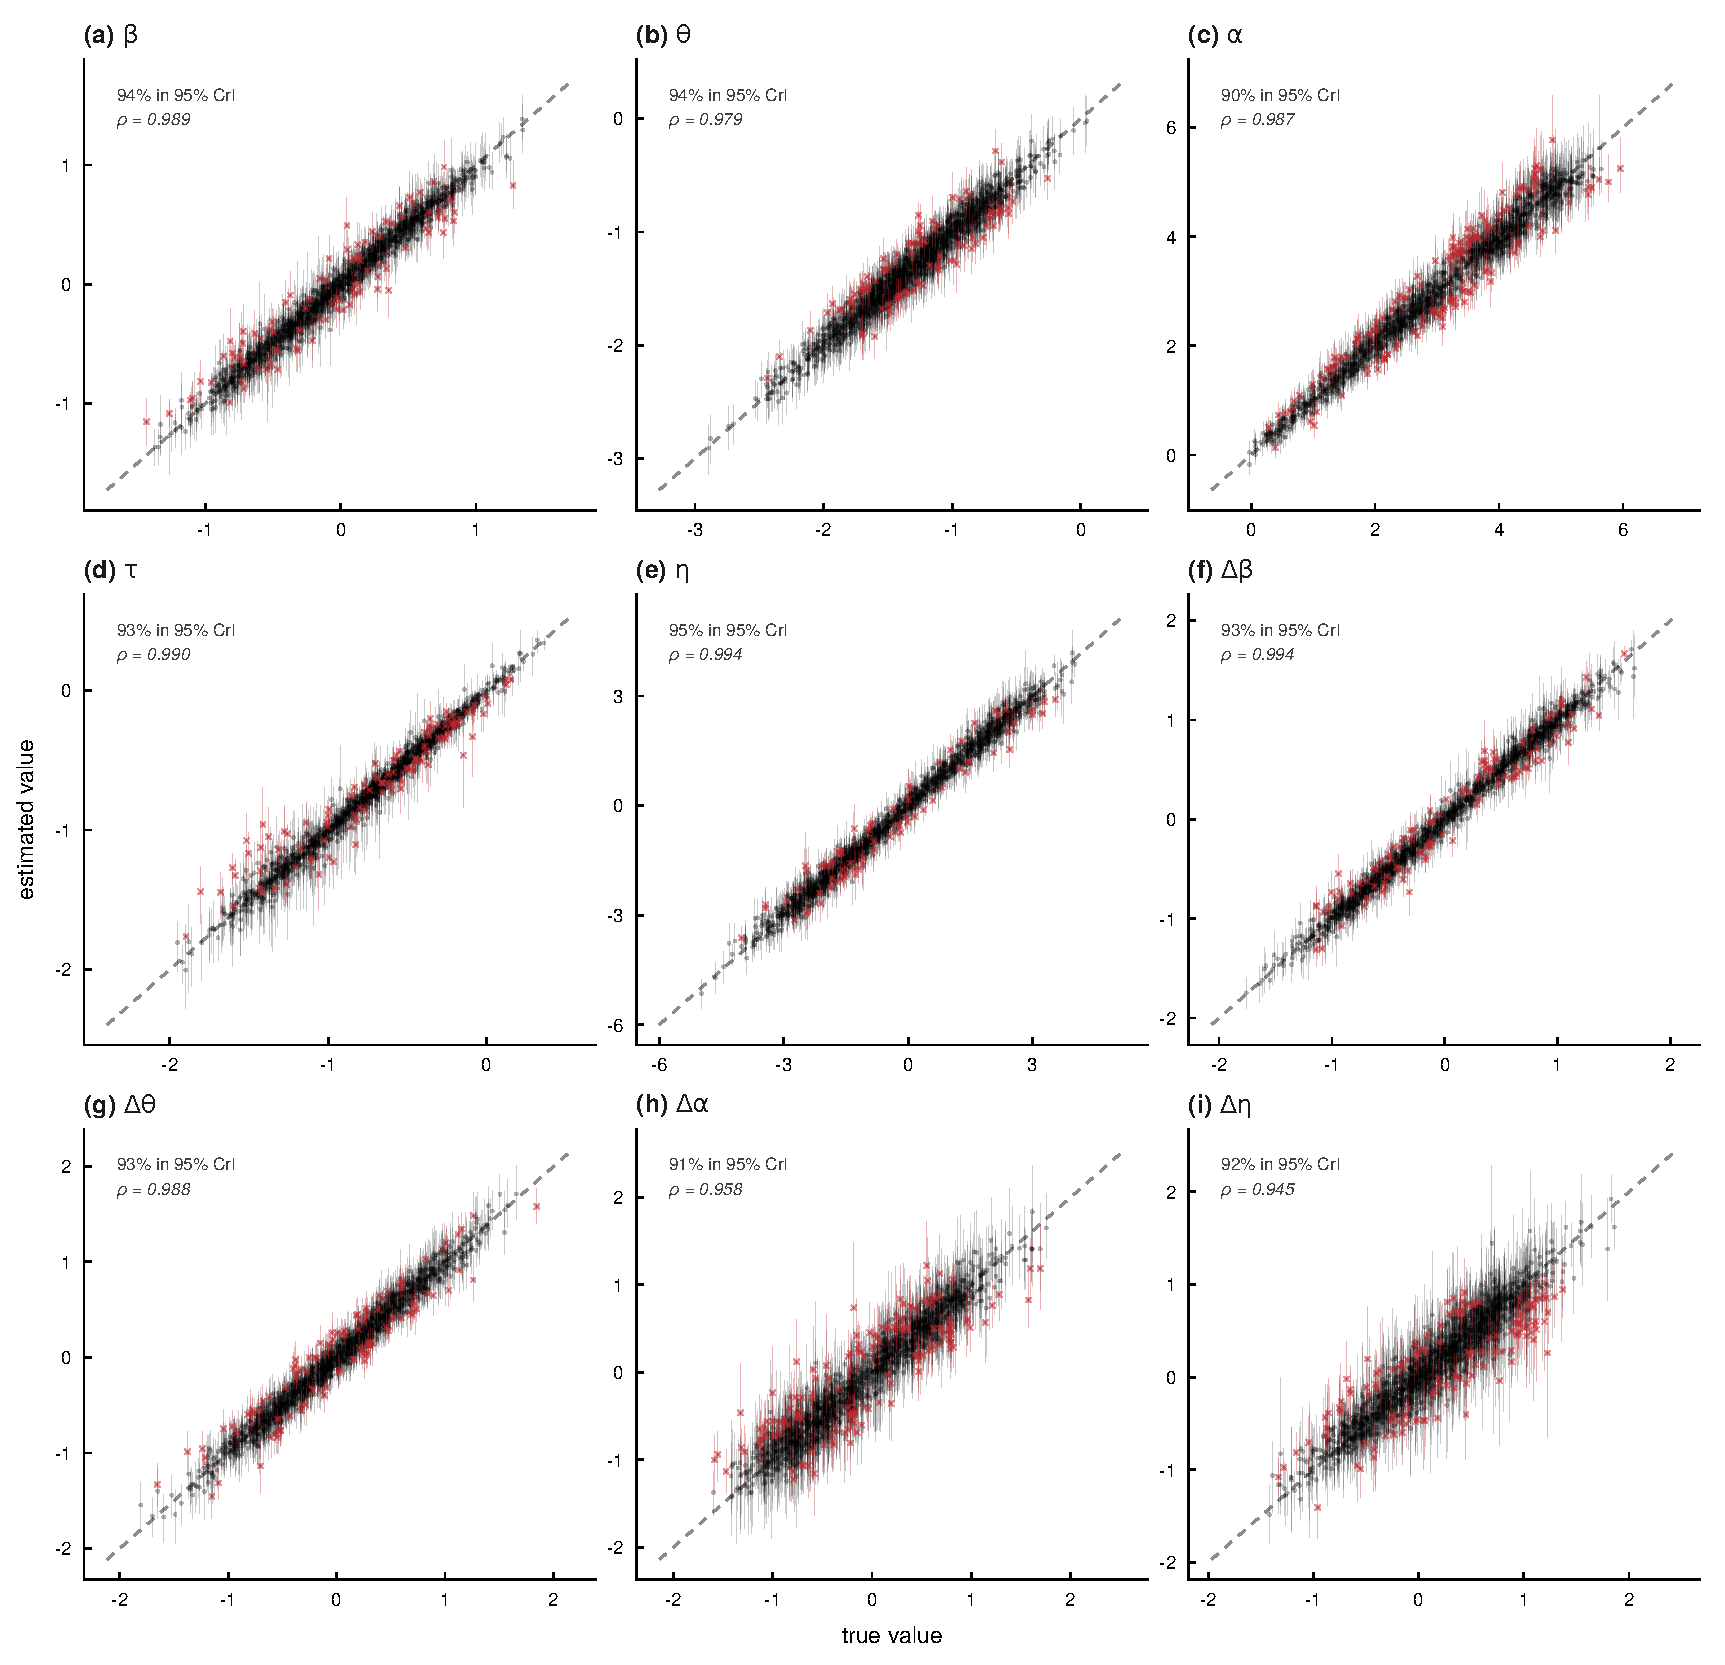
\includegraphics[width=\textwidth,height=0.58\textheight,keepaspectratio]{figures/mv_ccss_n_r_a_s_recovery.pdf}
    \end{center}
    \textit{Note.} Results are based on 50 simulated data sets of 30 participants each ($N = 1{,}500$ per parameter) generated from the Study 2 stimulus template. Each point represents one simulated participant. The $x$-axis shows the true generating value on the unconstrained scale; the $y$-axis shows the corresponding posterior mean. Vertical lines indicate 95\% Bayesian credible intervals, and the dashed diagonal marks perfect recovery. Red $\times$ markers indicate intervals that exclude the true value. The top-left badge of each panel reports the proportion of 95\% credible intervals that cover the true value (nominal rate = 95\%) and the Pearson correlation $\rho$ between true and estimated values.
\end{figure}

\begin{figure}[!htbp]
    \caption{Parameter recovery for the MVS CS model with starting-point bias and drift-rate adjustment}
    \label{fig:recovery_mvs_cs}
    \begin{center}
        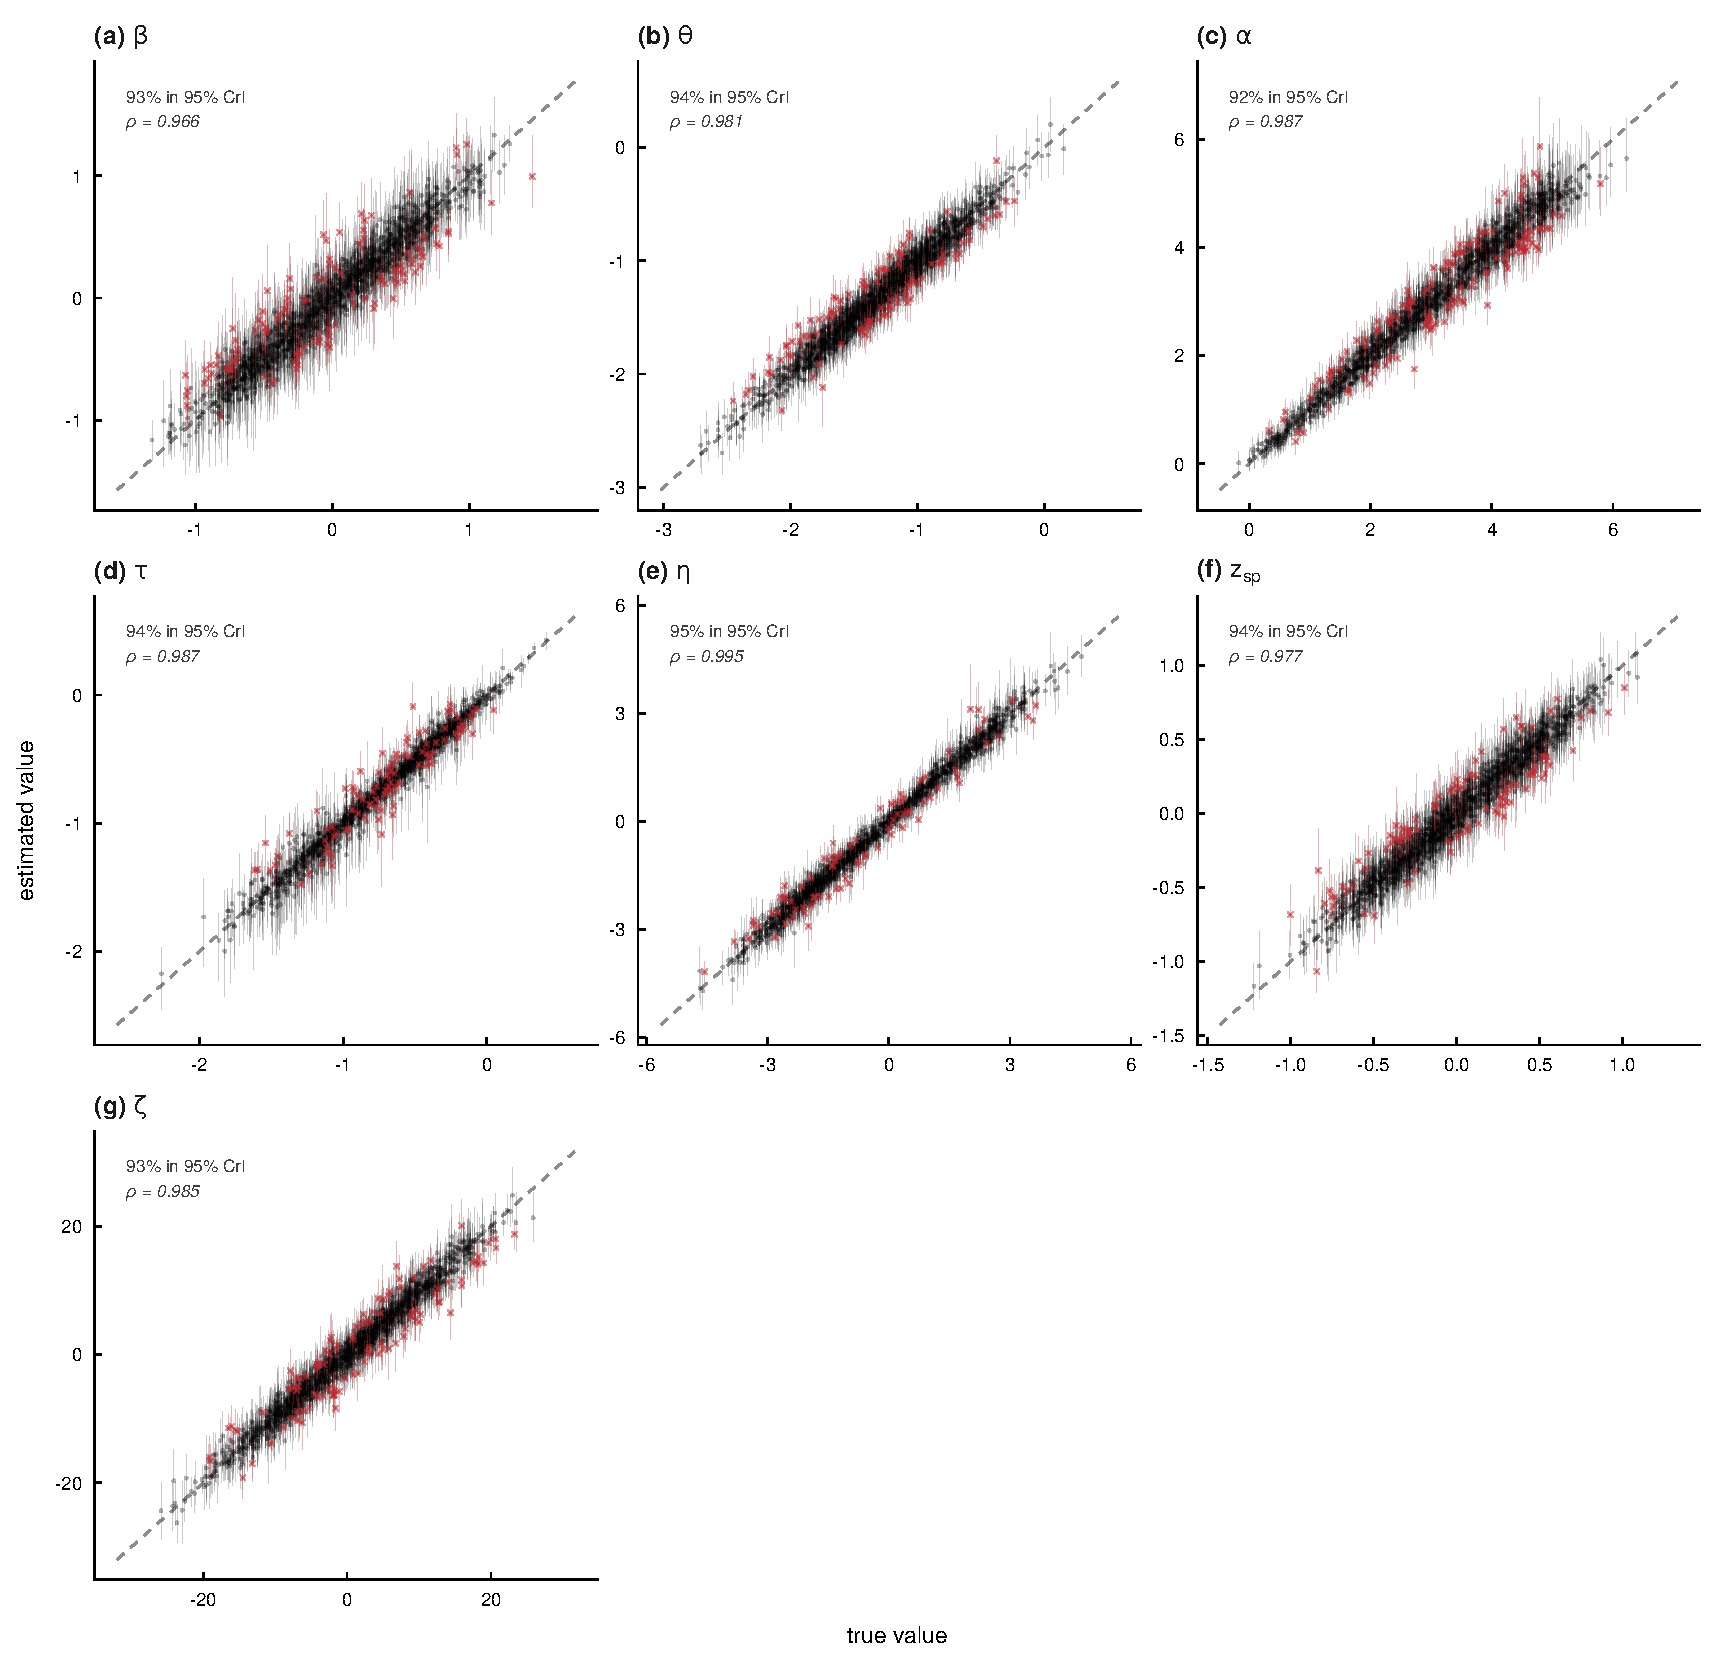
\includegraphics[width=\textwidth,height=0.58\textheight,keepaspectratio]{figures/mv_cs_sp_dr_recovery.pdf}
    \end{center}
    \textit{Note.} Results are based on 50 simulated data sets of 30 participants each ($N = 1{,}500$ per parameter) generated from the Study 2 stimulus template. Conventions are the same as in Figure~\ref{fig:recovery_mvs_ccss}.
\end{figure}

\subsubsection{CPT-Based Models}

Figures~\ref{fig:recovery_cpt_ccss} and \ref{fig:recovery_cpt_cs} present the corresponding per-participant true-versus-estimated scatter plots for the most complex CPT-based variant in each condition, with the same plotting conventions.

\begin{figure}[!htbp]
    \caption{Parameter recovery for the CPT CCSS model with all shift parameters}
    \label{fig:recovery_cpt_ccss}
    \begin{center}
        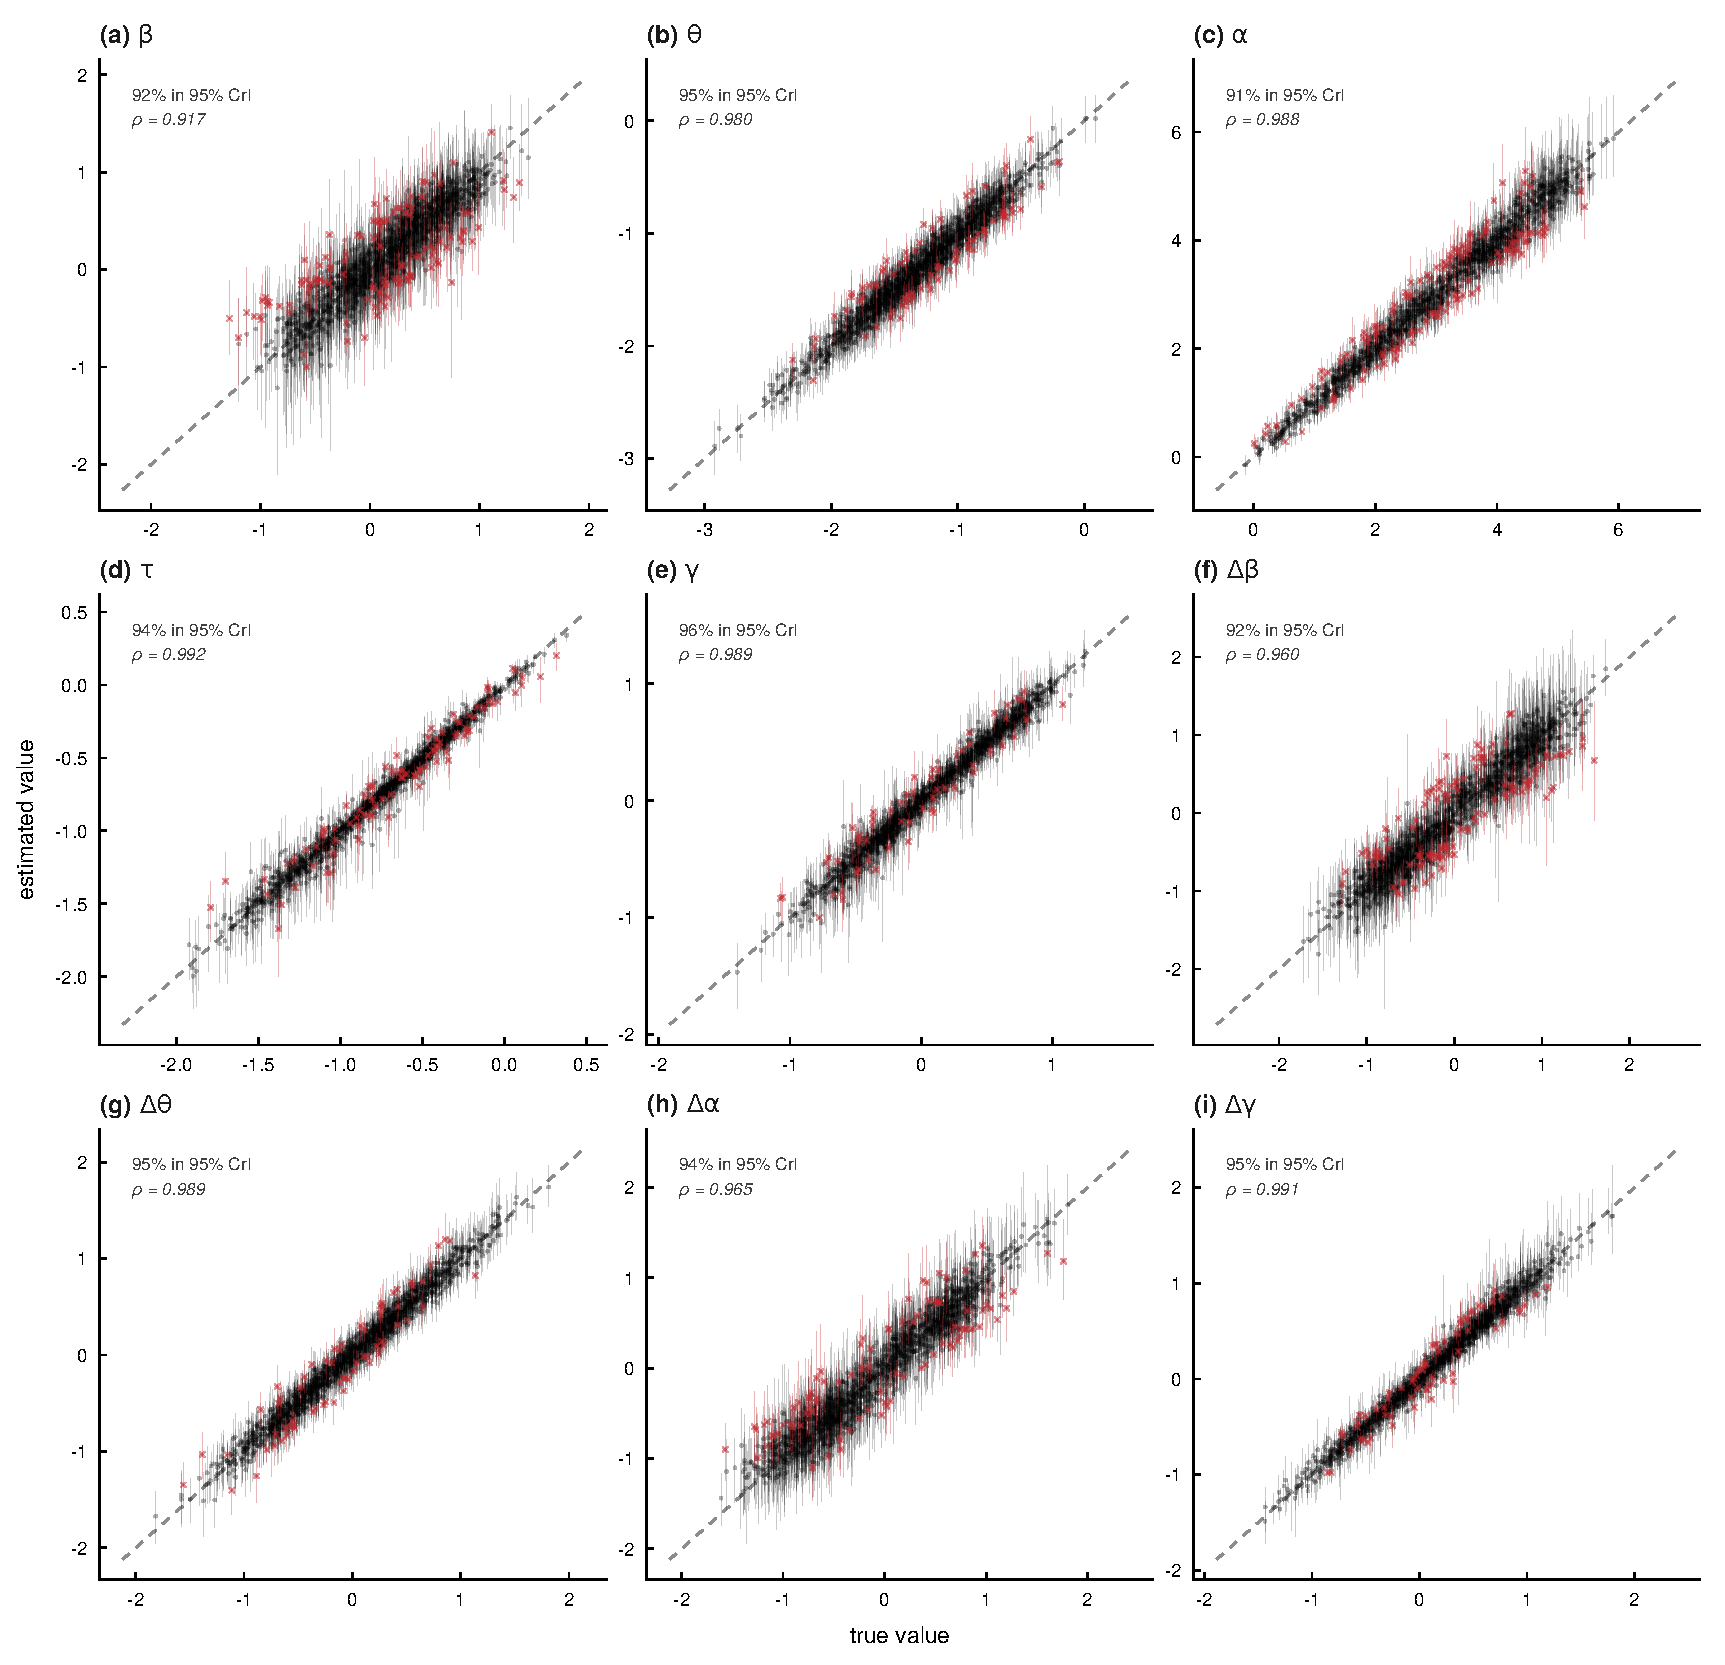
\includegraphics[width=\textwidth,height=0.58\textheight,keepaspectratio]{figures/cpt_ccss_n_r_a_s_recovery.pdf}
    \end{center}
    \textit{Note.} Results are based on 47 simulated data sets of 30 participants each ($N = 1{,}410$ per parameter) generated from the Study 2 stimulus template. Three of the 50 planned datasets were not fitted because the cluster wall-time limit was reached. The shift parameters are $\Delta_{\text{risk}}$, $\Delta_{\text{SNR}}$, $\Delta_{\text{threshold}}$, and $\Delta_{\text{PW}}$. Conventions are the same as in Figure~\ref{fig:recovery_mvs_ccss}.
\end{figure}

\begin{figure}[!htbp]
    \caption{Parameter recovery for the CPT CS model with starting-point bias and drift-rate adjustment}
    \label{fig:recovery_cpt_cs}
    \begin{center}
        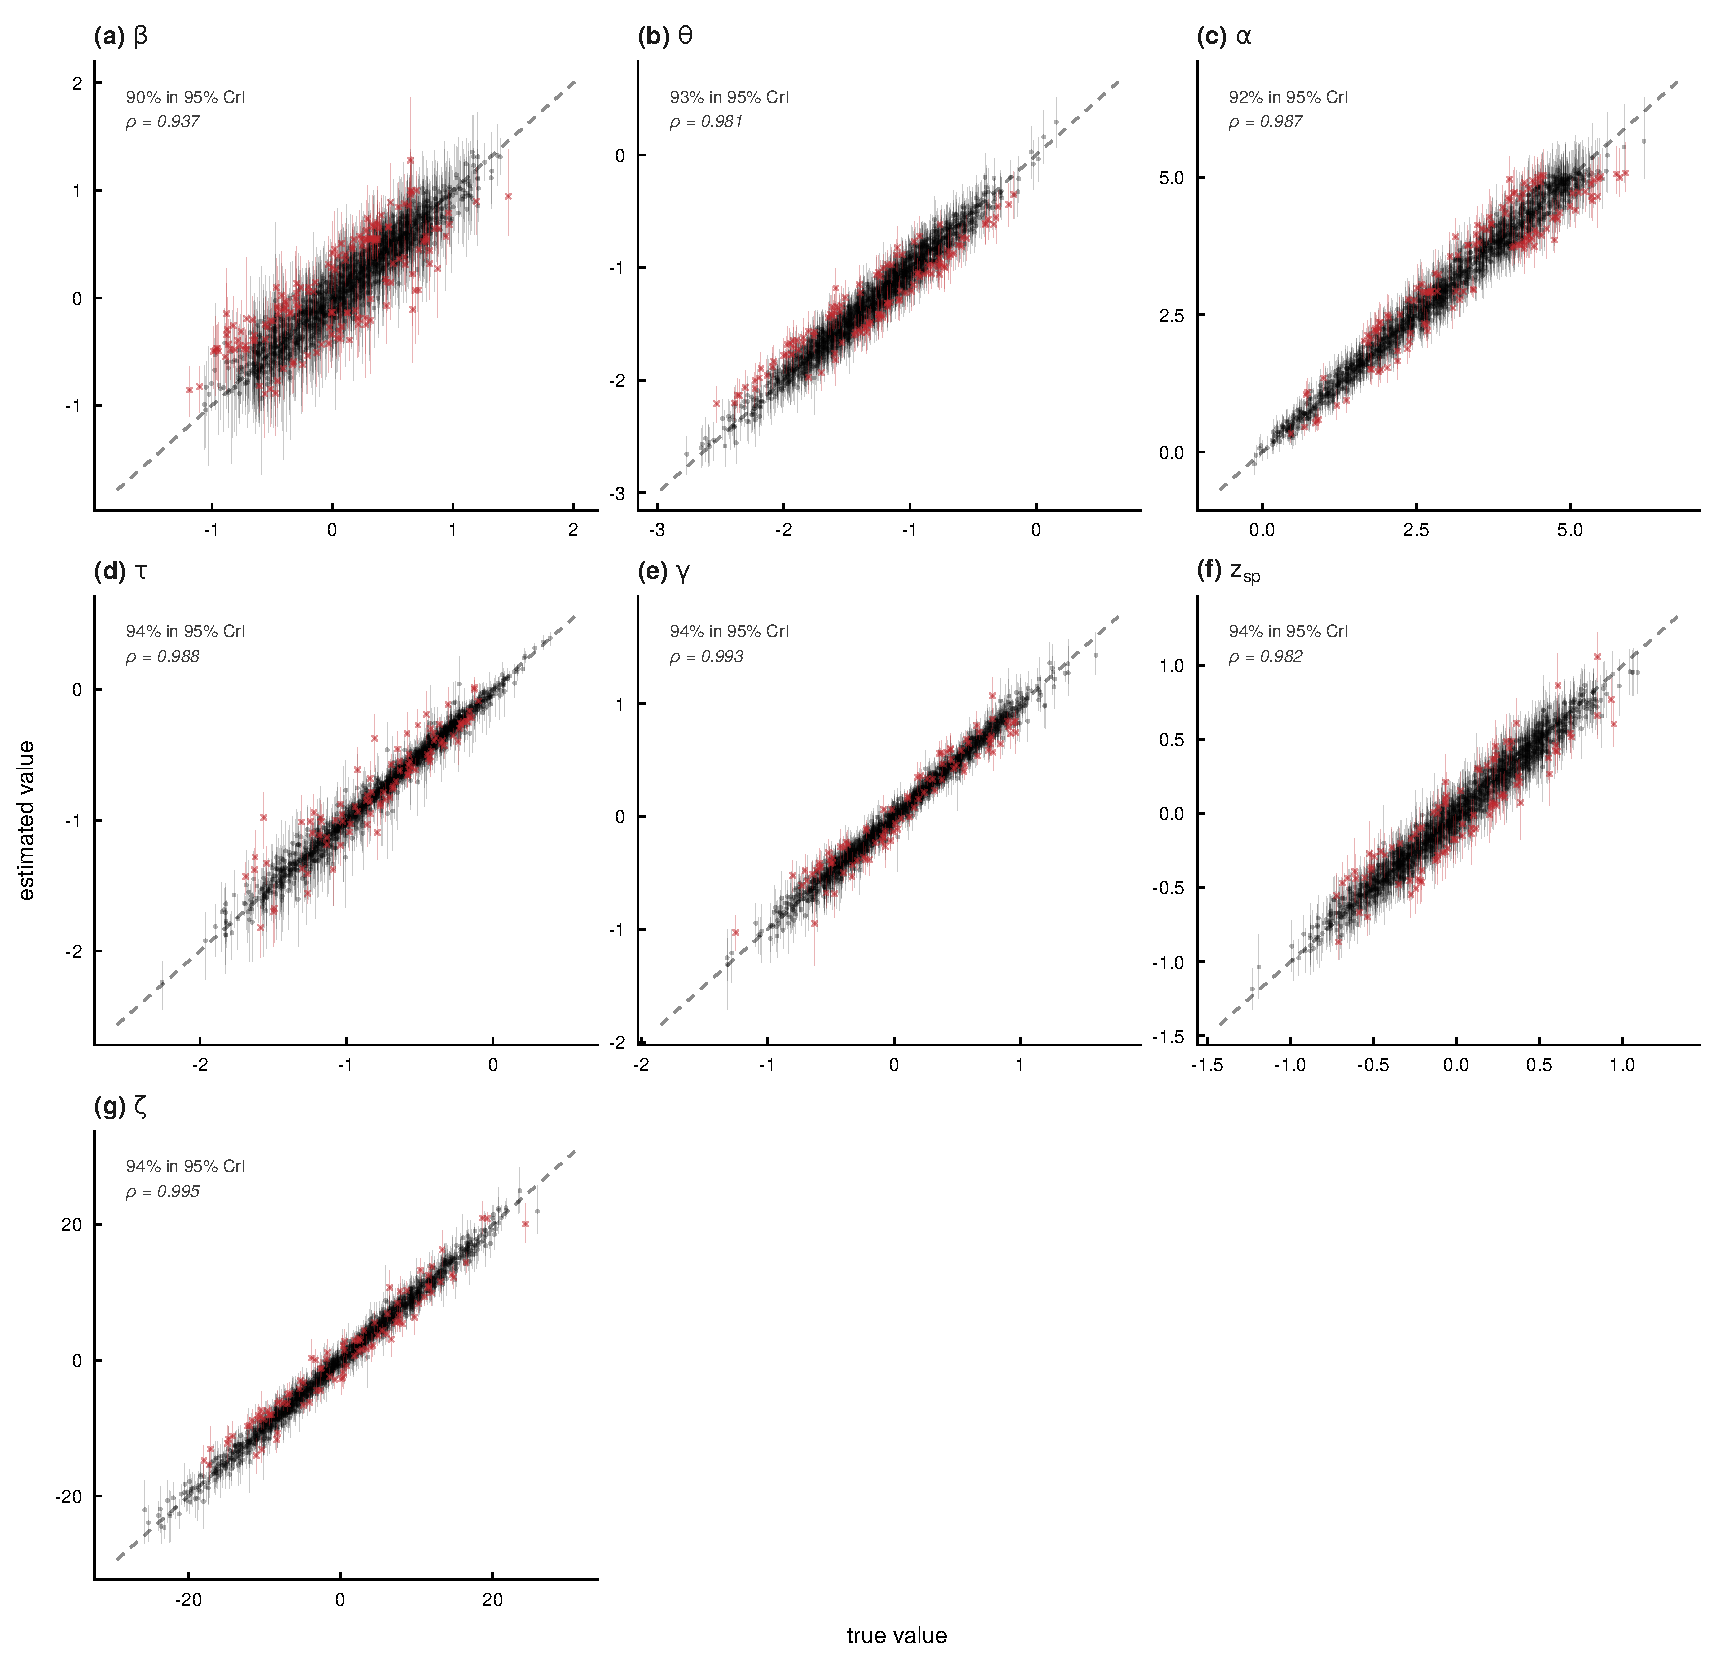
\includegraphics[width=\textwidth,height=0.58\textheight,keepaspectratio]{figures/cpt_cs_sp_dr_recovery.pdf}
    \end{center}
    \textit{Note.} Results are based on 50 simulated data sets of 30 participants each ($N = 1{,}500$ per parameter) generated from the Study 2 stimulus template. Conventions are the same as in Figure~\ref{fig:recovery_mvs_ccss}.
\end{figure}

\clearpage

\begin{table}[!htbp]
\centering
\begin{threeparttable}
\caption{Parameter Recovery Summary: Pearson Correlation ($\rho$) and 95\% CrI Coverage for Individual-Level Parameters}
\label{tab:recovery_summary}
\footnotesize
\setlength{\tabcolsep}{4pt}
\renewcommand{\arraystretch}{0.92}
\begin{tabularx}{\textwidth}{p{4.6cm}c*{4}{>{\centering\arraybackslash}X}}
\toprule
 & & \multicolumn{2}{c}{\textbf{MVS}} & \multicolumn{2}{c}{\textbf{CPT}} \\
\cmidrule(lr){3-4} \cmidrule(lr){5-6}
\textbf{Parameter} & \textbf{Symbol} & \textbf{$\rho$} & \textbf{Cov.} & \textbf{$\rho$} & \textbf{Cov.} \\
\midrule
\multicolumn{6}{l}{\textit{CCSS models (full shift model)}} \\
Risk pref.\ / Utility curv.   & $\beta$ / $\beta_{\text{CPT}}$ & .99 & 94\% & .92 & 92\% \\
Signal-to-noise ratio         & $\theta$                        & .98 & 94\% & .98 & 95\% \\
Decision threshold            & $\alpha$                        & .99 & 91\% & .99 & 91\% \\
Non-decision time             & $T_0$                           & .99 & 93\% & .99 & 94\% \\
Skewness pref.\ / Prob.\ wt.  & $\eta$ / $\gamma$               & .99 & 95\% & .99 & 96\% \\
Shift: risk / utility         & $\Delta_\beta$ / $\Delta_{\beta_{\text{CPT}}}$ & .99 & 93\% & .96 & 92\% \\
Shift: SNR                    & $\Delta_\theta$                 & .99 & 93\% & .99 & 95\% \\
Shift: threshold              & $\Delta_\alpha$                 & .96 & 91\% & .97 & 94\% \\
Shift: skewness / prob.\ wt.  & $\Delta_\eta$ / $\Delta_\gamma$ & .95 & 92\% & .99 & 95\% \\[4pt]
\multicolumn{6}{l}{\textit{CS models (starting-point bias and drift-rate adjustment)}} \\
Risk pref.\ / Utility curv.   & $\beta$ / $\beta_{\text{CPT}}$ & .97 & 93\% & .94 & 90\% \\
Signal-to-noise ratio         & $\theta$                        & .98 & 94\% & .98 & 93\% \\
Decision threshold            & $\alpha$                        & .99 & 92\% & .99 & 92\% \\
Non-decision time             & $T_0$                           & .99 & 94\% & .99 & 94\% \\
Skewness pref.\ / Prob.\ wt.  & $\eta$ / $\gamma$               & 1.00& 95\% & .99 & 94\% \\
Starting-point bias           & $z$                             & .98 & 94\% & .98 & 94\% \\
Drift-rate adjustment         & $\zeta$                         & .99 & 93\% & 1.00& 94\% \\
\bottomrule
\end{tabularx}
\begin{tablenotes}[flushleft]
\small
\item \textit{Note.} Each cell reports the Pearson correlation $\rho$ between true and posterior-mean parameter values (left of the slash for the MVS model, right of the slash for the CPT model in each row), pooled across all simulated participants, and the proportion of 95\% Bayesian credible intervals that cover the true value (Cov.; nominal rate = 95\%). All values are computed on the unconstrained (raw) scale. CCSS-model rows use 50 simulated datasets $\times$ 30 participants ($N = 1{,}500$) for MVS CCSS and 47 datasets ($N = 1{,}410$) for CPT CCSS; CS-model rows use 50 datasets ($N = 1{,}500$) for both variants. Correlations are rounded to two decimal places; values displayed as $1.00$ correspond to $\rho \geq .995$.
\end{tablenotes}
\end{threeparttable}
\end{table}

%% ============================================================================
\section{Group-Level Parameter Correlations (\texorpdfstring{$\boldsymbol{\Omega}$}{Omega})}
\label{sec:omega}
%% ============================================================================

Each hierarchical model includes a population-level correlation matrix $\boldsymbol{\Omega}$ over the individual random effects, estimated jointly with the group means $\mu_k$ and SDs $\sigma_k$ via a non-centred multivariate-normal parameterisation. The prior on $\boldsymbol{\Omega}$ is LKJ$(1)$ \parencite{lewandowski_generating_2009}, which places uniform density over the space of positive-definite correlation matrices. Figures~\ref{fig:omega_ccss} and~\ref{fig:omega_cs} show $\boldsymbol{\Omega}$ for the parsimony-best model in each (study, family) combination. Off-diagonal cells give posterior means; entries whose 95\% credible interval excludes zero are bolded; the diagonal is 1 by definition.

Most off-diagonal entries vary in sign or credibility across studies. We restrict our description to entries that take the same sign and are credibly nonzero in all three studies within at least one model class (CPT or MV). Two such patterns appear:

\begin{itemize}
\item The threshold $\alpha$ is positively correlated with the non-decision time $T_0$ in all three studies, in both model classes, and in both conditions (CCSS: posterior means $+.32$ to $+.56$; CS: $+.26$ to $+.64$; all credibly nonzero). Participants with higher decision thresholds tend to have longer non-decision times.
\item In the CCSS condition, $\alpha$ is positively correlated with its complexity shift $\Delta_{\text{threshold}}$ in all three studies in both model classes (posterior means $+.40$ to $+.56$; all credibly nonzero). Participants with higher baseline thresholds tend to show a larger upward shift in threshold under complexity.
\end{itemize}

Overall, the matrices show modest off-diagonal structure --- most cells are small and not credibly distinct from zero, no entry approaches $\pm 1$ in any combination, and we see no patterns that would indicate collinearity or non-identifiability at the population level.

\begin{landscape}
\begin{figure}[!htbp]
  \centering
  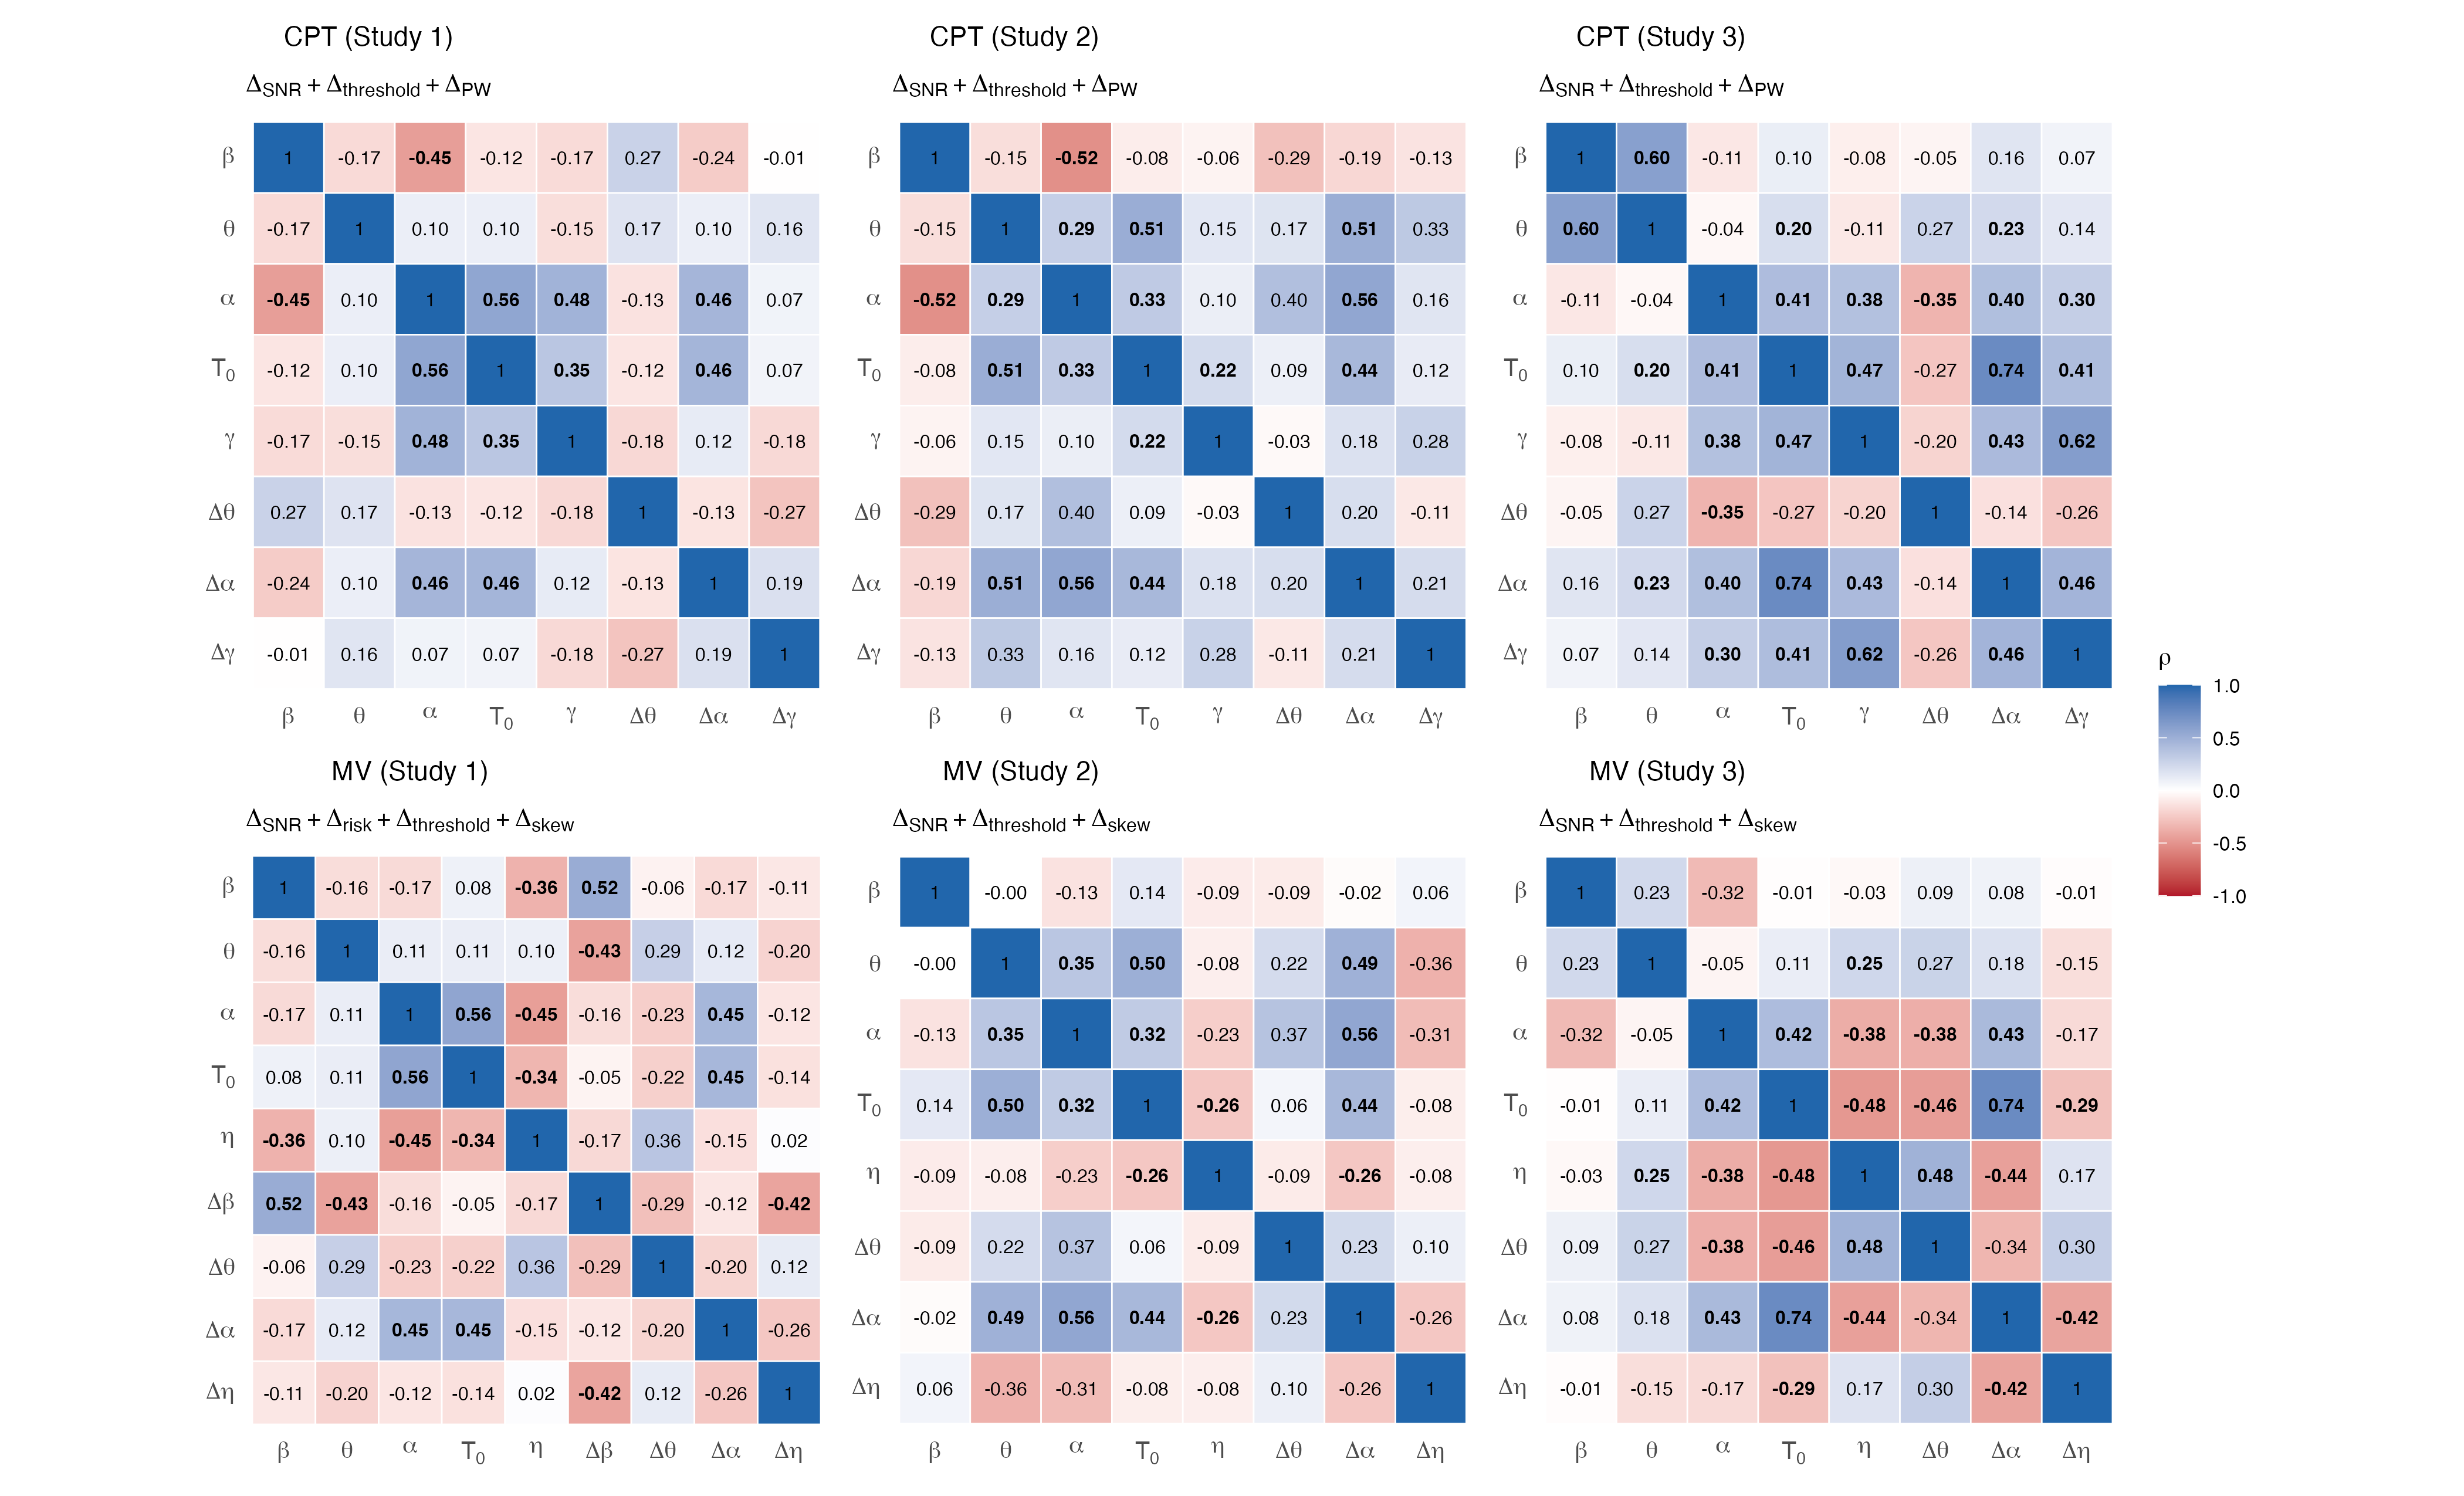
\includegraphics[width=0.95\linewidth]{figures/omega_best_CCSS.png}
  \caption{Posterior estimates of the population-level correlation matrix $\boldsymbol{\Omega}$ for the parsimony-best CCSS model in each (study, family) combination. Top row: CPT family. Bottom row: MV family. Cells show posterior means; entries with 95\% credible intervals excluding zero are bolded. The diagonal is 1 by definition. Prior: LKJ$(1)$ \parencite{lewandowski_generating_2009}.}
  \label{fig:omega_ccss}
\end{figure}
\end{landscape}

\begin{landscape}
\begin{figure}[!htbp]
  \centering
  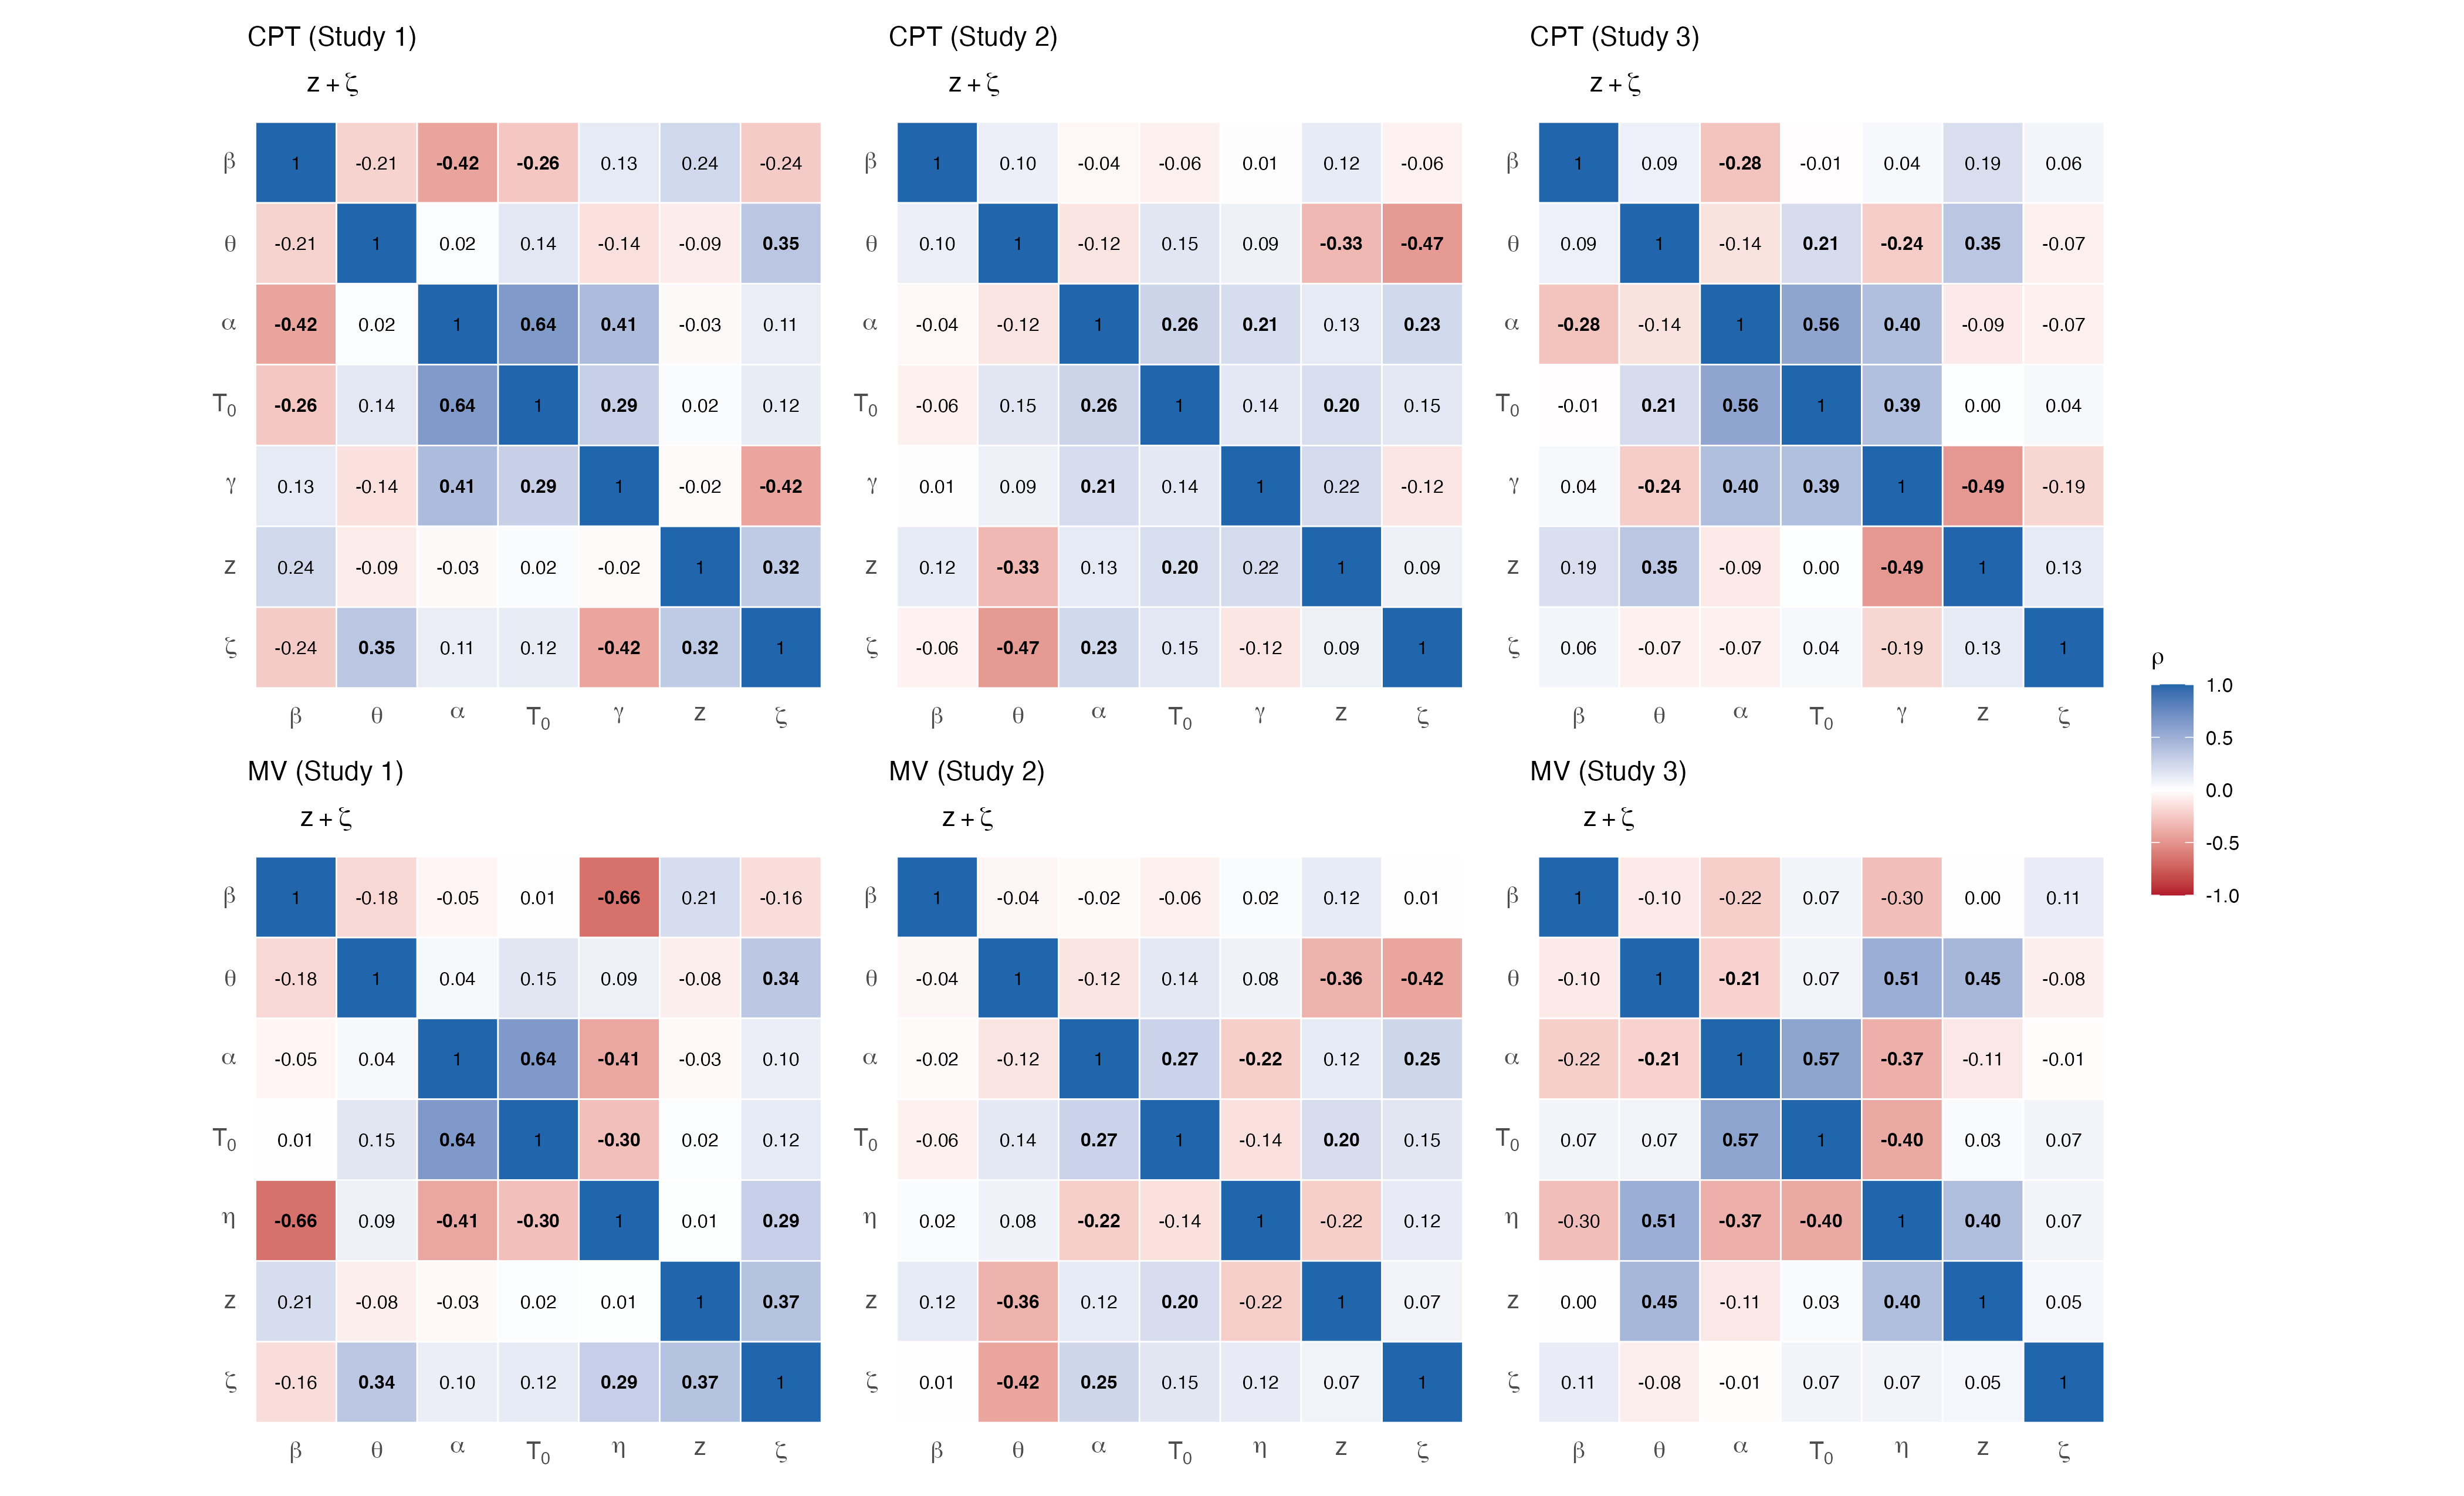
\includegraphics[width=0.95\linewidth]{figures/omega_best_CS.png}
  \caption{Posterior estimates of the population-level correlation matrix $\boldsymbol{\Omega}$ for the parsimony-best CS model ($z + \zeta$ in all six combinations). Top row: CPT family. Bottom row: MV family. Conventions as in Figure~\ref{fig:omega_ccss}.}
  \label{fig:omega_cs}
\end{figure}
\end{landscape}

\clearpage

%% ============================================================================
\section{CPT-Based Model Results}
\label{sec:cpt_results}
%% ============================================================================

As noted in the main text, the primary results are reported using the MVS utility representation. Here we present the full specification and results for models using cumulative prospect theory \parencite[CPT;][]{tversky_advances_1992} with \textcite{prelec_probability_1998} probability weighting. These models were fitted to the same data using the same hierarchical Bayesian procedure and serve as a robustness check for the conclusions drawn from the MVS-based analyses.

\subsection{CPT Value Representation}

Under cumulative prospect theory, the subjective utility of a two-outcome gamble $(o_1, p_1;\; o_2, p_2)$ with $o_1 \geq o_2$ is computed by applying a nonlinear probability weighting function and a power utility function to the raw outcomes and probabilities:
\begin{equation}
    U = w(p_1;\, \gamma) \cdot o_1^{\,\beta_{\text{CPT}}} + \bigl[1 - w(p_1;\, \gamma)\bigr] \cdot o_2^{\,\beta_{\text{CPT}}}
    \label{eq:cpt_utility}
\end{equation}
where $\beta_{\text{CPT}} > 0$ is the utility curvature parameter and $w(p;\, \gamma)$ is the \textcite{prelec_probability_1998} probability weighting function:
\begin{equation}
    w(p;\, \gamma) = \exp\!\bigl(-(-\ln p)^{\gamma}\bigr)
    \label{eq:prelec}
\end{equation}
with $\gamma > 0$ governing the degree of probability distortion. When $\gamma = 1$, probabilities are weighted linearly. When $\gamma < 1$, the classic inverse-S-shaped weighting pattern emerges: small probabilities are overweighted and large probabilities are underweighted.

The baseline drift rate is then defined as the scaled difference in utilities between the two options:
\begin{equation}
    v = \theta \cdot \bigl(U_A^{\,1/\beta_{\text{CPT}}} - U_B^{\,1/\beta_{\text{CPT}}}\bigr)
    \label{eq:cpt_drift}
\end{equation}
where the exponent $1/\beta_{\text{CPT}}$ rescales the utility back to the outcome scale, and $\theta > 0$ is the signal-to-noise ratio, as in the MVS models. The decision threshold $\alpha$ and non-decision time $T_0$ function identically to their MVS counterparts.

\subsection{CPT CCSS Models}

The hypotheses about how complexity affects the decision process are implemented in the CPT framework using the same shift-parameter logic as in the MVS models. For each base parameter $x$ with an associated shift parameter $\Delta_x$, the effective parameter on trial $n$ is modulated by the condition index $\text{con}_n \in \{-1, +1\}$. Because $\beta_{\text{CPT}}$, $\theta$, $\alpha$, and $\gamma$ are all constrained to be positive via the $\log(1 + e^{\cdot})$ transform, the shift operates inside the transform:
\begin{equation}
    x_{\text{eff},n} = \log\bigl(1 + \exp(x_{\text{raw}} + \Delta_x \cdot \text{con}_n)\bigr)
    \label{eq:cpt_delta}
\end{equation}

The four shift parameters and their interpretations parallel the MVS framework:
\begin{itemize}
    \item $\Delta_{\text{SNR}}$ (formally $\Delta_\theta$): A negative value indicates a reduced signal-to-noise ratio in complex (CC) relative to simple (SS) choice situations, leading to noisier evidence accumulation.
    \item $\Delta_{\text{threshold}}$ (formally $\Delta_\alpha$): A positive value indicates a higher decision threshold in complex situations, reflecting increased caution.
    \item $\Delta_{\text{risk}}$ (formally $\Delta_{\beta_{\text{CPT}}}$): Captures changes in utility curvature across complexity conditions. A shift in $\beta_{\text{CPT}}$ implies that the subjective transformation of outcomes changes with complexity.
    \item $\Delta_{\text{PW}}$ (formally $\Delta_\gamma$): Captures changes in probability weighting across complexity conditions. A shift in $\gamma$ implies that the degree of probability distortion differs between complex and simple gambles.
\end{itemize}

As in the MVS framework, all $2^4 = 16$ combinations of these four shift parameters were estimated, yielding models with 5 (baseline) to 9 (full) parameters per participant.

\subsection{CPT CS Models}

In the CS condition, the drift rate is computed as the difference in utilities between the complex and simple options, with an optional drift rate adjustment $\zeta$:
\begin{equation}
    v = \theta \cdot \bigl(U_{\text{complex}}^{\,1/\beta_{\text{CPT}}} - U_{\text{simple}}^{\,1/\beta_{\text{CPT}}} + \zeta\bigr)
    \label{eq:cpt_cs_drift}
\end{equation}
where a negative $\zeta$ biases the drift rate in favour of the simple option, analogous to the MVS CS specification.

The starting point bias $z = \Phi(z_{\text{raw}})$ functions identically to the MVS CS models: $z < 0.5$ reflects a pre-valuation bias toward the simple option.

By including or excluding the two mechanisms (starting point $z$ and drift rate adjustment $\zeta$), we obtained $2^2 = 4$ model variants (5 to 7 parameters per participant), matching the 4 CS models in the MVS framework: a baseline model with neither mechanism, two single-mechanism models ($z$ only and $\zeta$ only), and the full model combining both.

\subsection{CPT Model Comparison and Parameter Estimates}

We fitted the same 16 CCSS-condition models (all combinations of the four $\Delta$ shift parameters) and the same 4 CS-condition models (combinations of $z$ and $\zeta$) under the CPT value representation in each of the three studies. For every study, we report the full LOO-CV ranking and the group-level parameter estimates for the baseline and best-fitting model, separately for the CS and CCSS conditions, with prose that interprets the CPT results and compares them to the MVS-based estimates reported in the main text.

For the CCSS condition, the LOO-CV ranking places the full four-$\Delta$ model at rank~1 in all three studies. However, the parsimonious specification that drops $\Delta_{\text{risk}}$ and retains only $\Delta_{\text{SNR}}$, $\Delta_{\text{threshold}}$, and $\Delta_{\text{PW}}$ is statistically indistinguishable from the full model in all three studies ($|\Delta\widehat{\mathrm{elpd}}_{\mathrm{loo}}|/\mathrm{SE} = 0.5$, $1.2$, and $0.4$ for Studies~1, 2, and 3, all below the conventional $2 \times \mathrm{SE}$ threshold; \citealp{vehtari_practical_2017}). The next-best alternative is meaningfully worse in every study ($|\Delta|/\mathrm{SE} \geq 3.0$). We therefore report the parameter estimates of the parsimonious three-$\Delta$ model as the substantively preferred specification for the CCSS condition, consistent with the analogous absorption pattern documented for the MVS specification in the main text.

\subsubsection{Study 1}

\paragraph{CS condition.} As in the MVS analysis reported in the main text, the hierarchical Bayesian model comparison under the CPT representation favored the full CS specification incorporating both the starting-point bias ($z$) and the drift-rate adjustment ($\zeta$) over each single-mechanism alternative and over the baseline model (Table~\ref{tab:cpt_mc_cs_study1}; ELPD difference from the next-best $\zeta$-only model was $-55.3$, $\mathrm{SE} = 12.1$, $|\Delta|/\mathrm{SE} \approx 4.6$, meaningfully different). Parameter estimates from the full model (Table~\ref{tab:cpt_pe_cs_study1}) revealed a credible starting-point bias toward the simpler option (\textbf{$z = 0.49$}, 95\% CrI $[0.47, 0.50]$) and a credible drift-rate adjustment in the same direction (\textbf{$\zeta = -3.18$}, 95\% CrI $[-5.84, -0.61]$). Both effects are quantitatively close to and qualitatively identical with the MVS-based estimates reported in the main text ($z_{\text{MVS}} = 0.487$, $[0.475, 0.499]$; $\zeta_{\text{MVS}} = -4.70$, $[-7.47, -1.99]$). The slightly larger magnitude of $\zeta$ under the MVS specification arises because the MVS drift terms (EVD, SDD, SkewD) are on a larger numerical scale than the CPT-transformed value differences, so the same psychological bias requires a larger numerical $\zeta$ under MVS than under CPT. The conclusion is unchanged: in Study~1, the directed preference for the simpler option is jointly mediated by an anticipatory pre-valuation bias and an online drift-rate adjustment.

\begin{table}[!htbp]
\centering
\begin{threeparttable}\small
\caption{CPT model comparison using ELPD differences in the CS condition of Study~1}
\label{tab:cpt_mc_cs_study1}
\begin{tabularx}{\linewidth}{@{} >{\raggedright\arraybackslash}X rr @{}}
\toprule
\textbf{Model} & \textbf{ELPD difference} & \textbf{SE} \\
\midrule
Full (starting-point bias $z$, drift-rate adjustment $\zeta$) & 0.0 & 0.0 \\
Drift-rate adjustment only ($\zeta$) & $-55.3$ & 12.1 \\
Starting-point bias only ($z$) & $-374.5$ & 28.1 \\
Baseline (no extensions) & $-732.5$ & 35.4 \\
\bottomrule
\end{tabularx}
\begin{tablenotes}
\item \textit{Note.} ELPD differences are relative to the best-fitting model (set to 0); more positive values indicate better predictive accuracy. Following \textcite{vehtari_practical_2017}, an ELPD difference is considered meaningful only when $|\Delta\widehat{\mathrm{elpd}}_{\mathrm{loo}}|$ exceeds approximately $2 \times \mathrm{SE}$. 
\end{tablenotes}
\end{threeparttable}
\end{table}

\begin{table}[!htbp]
\centering
\begin{threeparttable}\small
\caption{Parameter estimates for baseline and best CPT models in the CS condition of Study~1}
\label{tab:cpt_pe_cs_study1}
\begin{tabularx}{\linewidth}{@{} >{\raggedright\arraybackslash}p{6cm} >{\centering\arraybackslash}X >{\centering\arraybackslash}X @{}}
\toprule
\textbf{Parameter} & \textbf{Baseline} & \textbf{Best model} \\
\midrule
$\beta_{\text{CPT}}$ (utility curvature) & $0.46$ $[0.20, 0.76]$ & $0.80$ $[0.51, 1.10]$ \\
$\theta$ (SNR) & $0.02$ $[0.02, 0.02]$ & $0.02$ $[0.02, 0.02]$ \\
$\alpha$ (threshold) & $3.84$ $[3.57, 4.12]$ & $4.00$ $[3.71, 4.29]$ \\
$T_0$ (non-decision time) & $1.23$ $[1.12, 1.35]$ & $1.24$ $[1.12, 1.36]$ \\
$\gamma$ (probability weighting) & $0.35$ $[0.28, 0.41]$ & $0.45$ $[0.39, 0.52]$ \\
$z$ (starting-point bias) & -- & \textbf{0.49} \textbf{[0.47, 0.50]} \\
$\zeta$ (drift-rate adjustment) & -- & \textbf{-3.18} \textbf{[-5.84, -0.61]} \\
\bottomrule
\end{tabularx}
\begin{tablenotes}
\item \textit{Note.} Values represent posterior means with 95\% credible intervals (CrIs). The Best Model refers to the full CS model including both the starting-point bias ($z$) and the drift-rate adjustment ($\zeta$). Parameters marked with ``--'' were not included in the corresponding model. Bold entries indicate parameters whose 95\% CrI excludes the relevant reference value (0 for $\Delta$ parameters and $\zeta$; 0.5 for $z$).
\end{tablenotes}
\end{threeparttable}
\end{table}

\paragraph{CCSS condition.} The LOO-CV ranking placed the full model (all four $\Delta$ shift parameters) at rank~1, but the ELPD difference between rank~1 and rank~2 (the more parsimonious model excluding $\Delta_{\text{risk}}$) was only $-2.0$ with $\mathrm{SE} = 3.9$ (Table~\ref{tab:cpt_mc_ccss_study1}). Because $|\Delta\widehat{\mathrm{elpd}}_{\mathrm{loo}}|/\mathrm{SE} = 0.5$ is well below the conventional $2 \times \mathrm{SE}$ threshold \parencite{vehtari_practical_2017}, the two specifications are statistically indistinguishable in predictive accuracy, and the more parsimonious model---which includes only $\Delta_{\text{SNR}}$, $\Delta_{\text{threshold}}$, and $\Delta_{\text{PW}}$---is the substantively preferred specification. The next-best alternative (rank~3) is meaningfully worse ($|\Delta\widehat{\mathrm{elpd}}_{\mathrm{loo}}|/\mathrm{SE} = 4.7$), so the parsimonious choice is well-supported by the data. Parameter estimates from this parsimonious model (Table~\ref{tab:cpt_pe_ccss_study1}) reproduced the two central effects identified in the MVS analysis: a credibly reduced signal-to-noise ratio in equally complex trials (\textbf{$\Delta_{\text{SNR}} = -0.22$}, $[-0.27, -0.17]$; MVS counterpart $\Delta_\theta = -0.20$, $[-0.25, -0.15]$) and a credibly elevated decision threshold (\textbf{$\Delta_{\text{threshold}} = 0.10$}, $[0.02, 0.18]$; MVS $\Delta_\alpha = 0.10$, $[0.02, 0.19]$). These two effects are quantitatively indistinguishable between the two representations, supporting the interpretation that the imprecision and compensatory deliberation effects of complexity are properties of the cognitive process rather than artefacts of the value model. The probability-weighting shift was credibly positive (\textbf{$\Delta_{\text{PW}} = 0.20$}, $[0.04, 0.35]$), indicating that the Prelec curvature parameter $\gamma$ is larger (closer to linear) in equally complex trials than in equally simple trials. Because smaller $\gamma$ corresponds to greater inverse-S distortion (and therefore stronger overweighting of small probabilities, which inflates the subjective value of right-skewed gambles), a positive $\Delta_{\text{PW}}$ implies that participants show \emph{less} overweighting of small probabilities under complexity and consequently a reduced behavioural preference for right-skewed options. This converges with the MVS analysis: the skewness-preference shift $\Delta_\eta$ was non-credible in the MVS full model ($-0.06$, $[-0.36, 0.25]$) but credibly negative when added alone ($-0.53$, $[-0.82, -0.22]$), reflecting a reduction in the apparent preference for right-skewed options in CC trials. Both frameworks therefore agree on the direction of the skewness-related effect, but the CPT framework localises it on the probability-weighting curvature rather than on a direct skewness moment. The risk-preference shift $\Delta_{\text{risk}}$ ($\Delta_{\beta_{\text{CPT}}}$) was credibly nonzero when included in the full model ($\Delta_{\text{risk}} = 0.59$, $[0.13, 1.17]$), but the LOO comparison indicates that the data do not support adding it as a separate mechanism beyond $\Delta_{\text{SNR}}$, $\Delta_{\text{threshold}}$, and $\Delta_{\text{PW}}$. This pattern parallels the MVS result, where $\Delta_\beta$ was also credible but its omission led to only a small loss in predictive accuracy. We therefore interpret $\Delta_{\text{risk}}$ as a quantitative refinement to model fit rather than as evidence for a genuine complexity-driven change in risk attitude.

\begin{table}[!htbp]
\centering
\begin{threeparttable}\small
\caption{CPT model comparison using ELPD differences in the CCSS condition of Study~1}
\label{tab:cpt_mc_ccss_study1}
\begin{tabularx}{\linewidth}{@{} >{\raggedright\arraybackslash}X rr @{}}
\toprule
\textbf{Model} & \textbf{ELPD difference} & \textbf{SE} \\
\midrule
Full model (shifts in all parameters: $\Delta\theta$, $\Delta\beta_{\text{CPT}}$, $\Delta\alpha$, $\Delta\gamma$) & 0.0 & 0.0 \\
Shift in SNR, threshold, PW ($\Delta\theta$, $\Delta\alpha$, $\Delta\gamma$) & $-2.0$ & 3.9 \\
Shift in SNR, risk, threshold ($\Delta\theta$, $\Delta\beta_{\text{CPT}}$, $\Delta\alpha$) & $-46.4$ & 10.0 \\
Shift in SNR, threshold ($\Delta\theta$, $\Delta\alpha$) & $-52.4$ & 11.1 \\
Shift in risk, threshold, PW ($\Delta\beta_{\text{CPT}}$, $\Delta\alpha$, $\Delta\gamma$) & $-79.2$ & 13.3 \\
Shift in threshold, PW ($\Delta\alpha$, $\Delta\gamma$) & $-80.9$ & 14.0 \\
Shift in risk, threshold ($\Delta\beta_{\text{CPT}}$, $\Delta\alpha$) & $-171.9$ & 19.3 \\
Shift in SNR, PW ($\Delta\theta$, $\Delta\gamma$) & $-178.2$ & 17.9 \\
Shift in SNR, risk, PW ($\Delta\theta$, $\Delta\beta_{\text{CPT}}$, $\Delta\gamma$) & $-178.2$ & 17.6 \\
Shift in threshold ($\Delta\alpha$) & $-190.3$ & 20.6 \\
Shift in SNR, risk ($\Delta\theta$, $\Delta\beta_{\text{CPT}}$) & $-222.0$ & 19.9 \\
Shift in SNR ($\Delta\theta$) & $-222.9$ & 20.4 \\
Shift in risk, PW ($\Delta\beta_{\text{CPT}}$, $\Delta\gamma$) & $-346.7$ & 23.5 \\
Shift in PW ($\Delta\gamma$) & $-352.2$ & 23.9 \\
Shift in risk ($\Delta\beta_{\text{CPT}}$) & $-476.6$ & 28.3 \\
Baseline (no parameter shifts) & $-506.7$ & 29.4 \\
\bottomrule
\end{tabularx}
\begin{tablenotes}
\item \textit{Note.} Sixteen models were compared, sorted by LOO-CV rank. ELPD differences are relative to the best-fitting model (set to 0); more positive values indicate better predictive accuracy. Following \textcite{vehtari_practical_2017}, an ELPD difference is considered meaningful only when $|\Delta\widehat{\mathrm{elpd}}_{\mathrm{loo}}|$ exceeds approximately $2 \times \mathrm{SE}$. 
\end{tablenotes}
\end{threeparttable}
\end{table}

\begin{table}[!htbp]
\centering
\begin{threeparttable}\small
\caption{Parameter estimates for baseline and parsimonious best CPT model in the CCSS condition of Study~1}
\label{tab:cpt_pe_ccss_study1}
\begin{tabularx}{\linewidth}{@{} >{\raggedright\arraybackslash}p{6cm} >{\centering\arraybackslash}X >{\centering\arraybackslash}X @{}}
\toprule
\textbf{Parameter} & \textbf{Baseline} & \textbf{Best model} \\
\midrule
$\beta_{\text{CPT}}$ (utility curvature) & $1.15$ $[0.82, 1.50]$ & $0.85$ $[0.44, 1.28]$ \\
$\theta$ (SNR) & $0.02$ $[0.02, 0.02]$ & $0.02$ $[0.02, 0.02]$ \\
$\alpha$ (threshold) & $4.09$ $[3.83, 4.36]$ & $4.13$ $[3.86, 4.40]$ \\
$T_0$ (non-decision time) & $1.21$ $[1.09, 1.33]$ & $1.25$ $[1.13, 1.37]$ \\
$\gamma$ (probability weighting) & $0.46$ $[0.40, 0.52]$ & $0.41$ $[0.34, 0.49]$ \\
$\Delta_{\text{SNR}}$ ($\Delta\theta$, SNR shift) & -- & \textbf{-0.22} \textbf{[-0.27, -0.17]} \\
$\Delta_{\text{threshold}}$ ($\Delta\alpha$, threshold shift) & -- & \textbf{0.10} \textbf{[0.02, 0.18]} \\
$\Delta_{\text{PW}}$ ($\Delta\gamma$, probability-weighting shift) & -- & \textbf{0.20} \textbf{[0.04, 0.35]} \\
\bottomrule
\end{tabularx}
\begin{tablenotes}
\item \textit{Note.} Values represent posterior means with 95\% credible intervals (CrIs). The Best Model refers to the parsimonious model including the SNR, threshold, and probability-weighting shifts ($\Delta_{\text{SNR}}+\Delta_{\text{threshold}}+\Delta_{\text{PW}}$). Although the LOO ranking placed the full model (including also $\Delta_{\text{risk}}$) at rank~1, the difference between rank~1 and rank~2 in this study was below the conventional $2 \times \mathrm{SE}$ threshold (see prose), so the more parsimonious model is reported here as the substantively preferred specification. Parameters marked with ``--'' were not included in the corresponding model. Bold entries indicate parameters whose 95\% CrI excludes the relevant reference value (0 for $\Delta$ parameters and $\zeta$; 0.5 for $z$).
\end{tablenotes}
\end{threeparttable}
\end{table}

\FloatBarrier

\subsubsection{Study 2}

\paragraph{CS condition.} As in Study~1, the LOO-CV comparison favored the full CS model with both the starting-point bias and the drift-rate adjustment over the single-mechanism alternatives and the baseline (Table~\ref{tab:cpt_mc_cs_study2}; ELPD difference from the next-best $\zeta$-only model was $-298.7$, $\mathrm{SE} = 26.0$, $|\Delta|/\mathrm{SE} \approx 11.5$, meaningfully different). Parameter estimates from the best-fitting model (Table~\ref{tab:cpt_pe_cs_study2}) showed a strong pre-valuation bias toward the simpler option (\textbf{$z = 0.42$}, 95\% CrI $[0.41, 0.44]$) and a substantial drift-rate adjustment in the same direction (\textbf{$\zeta = -10.53$}, 95\% CrI $[-14.06, -6.89]$). Both effects mirror the MVS-based estimates ($z_{\text{MVS}} = 0.42$, $[0.41, 0.44]$; $\zeta_{\text{MVS}} = -13.12$, $[-17.13, -9.18]$) and replicate the Study~1 pattern. The pre-valuation bias is notably stronger in Study~2 than in Study~1 ($z \approx 0.42$ vs.\ $z \approx 0.49$) under both value representations, consistent with the interpretation that the arithmetic-expression complexity used in Study~2 produces a more salient cue to participants that the complex option is harder to evaluate before they begin to integrate evidence, and consequently a stronger anticipatory shift in the starting point.

\begin{table}[!htbp]
\centering
\begin{threeparttable}\small
\caption{CPT model comparison using ELPD differences in the CS condition of Study~2}
\label{tab:cpt_mc_cs_study2}
\begin{tabularx}{\linewidth}{@{} >{\raggedright\arraybackslash}X rr @{}}
\toprule
\textbf{Model} & \textbf{ELPD difference} & \textbf{SE} \\
\midrule
Full (starting-point bias $z$, drift-rate adjustment $\zeta$) & 0.0 & 0.0 \\
Drift-rate adjustment only ($\zeta$) & $-298.7$ & 26.0 \\
Baseline (no extensions) & $-1420.5$ & 46.3 \\
\bottomrule
\end{tabularx}
\begin{tablenotes}
\item \textit{Note.} ELPD differences are relative to the best-fitting model (set to 0); more positive values indicate better predictive accuracy. Following \textcite{vehtari_practical_2017}, an ELPD difference is considered meaningful only when $|\Delta\widehat{\mathrm{elpd}}_{\mathrm{loo}}|$ exceeds approximately $2 \times \mathrm{SE}$. The starting-point-only model ($z$) did not converge under any of the sampler configurations attempted (see the \nameref{sec:convergence} section) and is omitted. 
\end{tablenotes}
\end{threeparttable}
\end{table}

\begin{table}[!htbp]
\centering
\begin{threeparttable}\small
\caption{Parameter estimates for baseline and best CPT models in the CS condition of Study~2}
\label{tab:cpt_pe_cs_study2}
\begin{tabularx}{\linewidth}{@{} >{\raggedright\arraybackslash}p{6cm} >{\centering\arraybackslash}X >{\centering\arraybackslash}X @{}}
\toprule
\textbf{Parameter} & \textbf{Baseline} & \textbf{Best model} \\
\midrule
$\beta_{\text{CPT}}$ (utility curvature) & $0.62$ $[0.36, 0.88]$ & $0.62$ $[0.36, 0.85]$ \\
$\theta$ (SNR) & $0.01$ $[0.00, 0.01]$ & $0.01$ $[0.01, 0.01]$ \\
$\alpha$ (threshold) & $4.74$ $[4.41, 5.07]$ & $5.14$ $[4.82, 5.45]$ \\
$T_0$ (non-decision time) & $1.07$ $[0.76, 1.43]$ & $1.36$ $[1.03, 1.71]$ \\
$\gamma$ (probability weighting) & $0.79$ $[0.62, 0.97]$ & $0.75$ $[0.60, 0.91]$ \\
$z$ (starting-point bias) & -- & \textbf{0.42} \textbf{[0.41, 0.44]} \\
$\zeta$ (drift-rate adjustment) & -- & \textbf{-10.53} \textbf{[-14.06, -6.89]} \\
\bottomrule
\end{tabularx}
\begin{tablenotes}
\item \textit{Note.} Values represent posterior means with 95\% credible intervals (CrIs). The Best Model refers to the full CS model including both the starting-point bias ($z$) and the drift-rate adjustment ($\zeta$). Parameters marked with ``--'' were not included in the corresponding model. Bold entries indicate parameters whose 95\% CrI excludes the relevant reference value (0 for $\Delta$ parameters and $\zeta$; 0.5 for $z$).
\end{tablenotes}
\end{threeparttable}
\end{table}

\paragraph{CCSS condition.} As in Study~1, the LOO-CV ranking placed the full model at rank~1 but the difference between rank~1 and rank~2 (the model excluding $\Delta_{\text{risk}}$) was below the $2 \times \mathrm{SE}$ threshold ($\Delta\widehat{\mathrm{elpd}}_{\mathrm{loo}} = -5.4$, $\mathrm{SE} = 4.4$, $|\Delta|/\mathrm{SE} = 1.2$; Table~\ref{tab:cpt_mc_ccss_study2}). The two specifications are therefore statistically indistinguishable, and the parsimonious model excluding $\Delta_{\text{risk}}$ is the substantively preferred specification. The next alternative (rank~3) is meaningfully worse ($|\Delta|/\mathrm{SE} = 3.0$). Parameter estimates from the parsimonious model (Table~\ref{tab:cpt_pe_ccss_study2}) showed a substantially larger signal-to-noise reduction than in Study~1 (\textbf{$\Delta_{\text{SNR}} = -0.90$}, $[-1.06, -0.79]$; MVS counterpart $\Delta_\theta = -0.90$, $[-1.04, -0.79]$) and a larger threshold elevation (\textbf{$\Delta_{\text{threshold}} = 0.46$}, $[0.31, 0.61]$; MVS $\Delta_\alpha = 0.46$, $[0.31, 0.60]$). Both effects are quantitatively close to the MVS counterparts and indicate that the arithmetic-expression manipulation imposes a substantially larger cognitive load on evidence accumulation than the number-of-outcomes manipulation of Study~1. The probability-weighting shift was credibly positive (\textbf{$\Delta_{\text{PW}} = 0.46$}, $[0.20, 0.73]$), again indicating that $\gamma$ moves closer to linear (less inverse-S distortion) in complex trials. As in Study~1, this implies that participants show less overweighting of small probabilities and consequently a reduced behavioural preference for right-skewed gambles in CC trials. The MVS analysis shows a parallel signature: the skewness-preference shift $\Delta_\eta$ was borderline non-credible in the full model ($-0.72$, $[-1.40, 0.005]$) but credibly negative when added alone ($-3.19$, $[-3.99, -2.41]$). Both frameworks again agree on the direction of the skewness-related effect, with the CPT representation reading it as a flatter probability-weighting curve under complexity and the MVS representation reading it as a direct reduction in the skewness-difference weight. As in Study~1, the risk-preference shift was credibly positive in the full CPT model ($\Delta_{\text{risk}} = 1.00$, $[0.39, 1.67]$) but the LOO comparison did not support adding it as a separate mechanism beyond the parsimonious three-$\Delta$ specification. The same pattern holds in the MVS specification ($\Delta_\beta = 0.16$, $[0.03, 0.30]$, credibly positive but largely redundant with the SNR reduction), strengthening the conclusion that the apparent risk-preference change is a quantitative refinement absorbed by the reduced sensitivity to value differences.

\begin{table}[!htbp]
\centering
\begin{threeparttable}\small
\caption{CPT model comparison using ELPD differences in the CCSS condition of Study~2}
\label{tab:cpt_mc_ccss_study2}
\begin{tabularx}{\linewidth}{@{} >{\raggedright\arraybackslash}X rr @{}}
\toprule
\textbf{Model} & \textbf{ELPD difference} & \textbf{SE} \\
\midrule
Full model (shifts in all parameters: $\Delta\theta$, $\Delta\beta_{\text{CPT}}$, $\Delta\alpha$, $\Delta\gamma$) & 0.0 & 0.0 \\
Shift in SNR, threshold, PW ($\Delta\theta$, $\Delta\alpha$, $\Delta\gamma$) & $-5.4$ & 4.4 \\
Shift in SNR, risk, threshold ($\Delta\theta$, $\Delta\beta_{\text{CPT}}$, $\Delta\alpha$) & $-23.4$ & 7.9 \\
Shift in SNR, threshold ($\Delta\theta$, $\Delta\alpha$) & $-35.9$ & 9.2 \\
Shift in risk, threshold, PW ($\Delta\beta_{\text{CPT}}$, $\Delta\alpha$, $\Delta\gamma$) & $-304.9$ & 24.3 \\
Shift in threshold, PW ($\Delta\alpha$, $\Delta\gamma$) & $-375.9$ & 26.7 \\
Shift in risk, threshold ($\Delta\beta_{\text{CPT}}$, $\Delta\alpha$) & $-593.3$ & 32.9 \\
Shift in SNR, risk, PW ($\Delta\theta$, $\Delta\beta_{\text{CPT}}$, $\Delta\gamma$) & $-652.9$ & 30.3 \\
Shift in SNR, PW ($\Delta\theta$, $\Delta\gamma$) & $-658.4$ & 30.4 \\
Shift in SNR, risk ($\Delta\theta$, $\Delta\beta_{\text{CPT}}$) & $-672.0$ & 31.0 \\
Shift in SNR ($\Delta\theta$) & $-681.6$ & 31.2 \\
Shift in threshold ($\Delta\alpha$) & $-802.3$ & 36.4 \\
Shift in risk, PW ($\Delta\beta_{\text{CPT}}$, $\Delta\gamma$) & $-1184.4$ & 39.3 \\
Shift in PW ($\Delta\gamma$) & $-1282.7$ & 41.3 \\
Shift in risk ($\Delta\beta_{\text{CPT}}$) & $-1643.3$ & 47.5 \\
Baseline (no parameter shifts) & $-1935.9$ & 51.0 \\
\bottomrule
\end{tabularx}
\begin{tablenotes}
\item \textit{Note.} Sixteen models were compared, sorted by LOO-CV rank. ELPD differences are relative to the best-fitting model (set to 0); more positive values indicate better predictive accuracy. Following \textcite{vehtari_practical_2017}, an ELPD difference is considered meaningful only when $|\Delta\widehat{\mathrm{elpd}}_{\mathrm{loo}}|$ exceeds approximately $2 \times \mathrm{SE}$. 
\end{tablenotes}
\end{threeparttable}
\end{table}

\begin{table}[!htbp]
\centering
\begin{threeparttable}\small
\caption{Parameter estimates for baseline and parsimonious best CPT model in the CCSS condition of Study~2}
\label{tab:cpt_pe_ccss_study2}
\begin{tabularx}{\linewidth}{@{} >{\raggedright\arraybackslash}p{6cm} >{\centering\arraybackslash}X >{\centering\arraybackslash}X @{}}
\toprule
\textbf{Parameter} & \textbf{Baseline} & \textbf{Best model} \\
\midrule
$\beta_{\text{CPT}}$ (utility curvature) & $0.82$ $[0.62, 1.03]$ & $0.54$ $[0.38, 0.69]$ \\
$\theta$ (SNR) & $0.01$ $[0.01, 0.01]$ & $0.01$ $[0.01, 0.01]$ \\
$\alpha$ (threshold) & $4.80$ $[4.55, 5.06]$ & $4.85$ $[4.59, 5.12]$ \\
$T_0$ (non-decision time) & $1.11$ $[0.95, 1.28]$ & $1.33$ $[1.15, 1.51]$ \\
$\gamma$ (probability weighting) & $0.58$ $[0.49, 0.68]$ & $0.77$ $[0.61, 0.96]$ \\
$\Delta_{\text{SNR}}$ ($\Delta\theta$, SNR shift) & -- & \textbf{-0.90} \textbf{[-1.06, -0.79]} \\
$\Delta_{\text{threshold}}$ ($\Delta\alpha$, threshold shift) & -- & \textbf{0.46} \textbf{[0.31, 0.61]} \\
$\Delta_{\text{PW}}$ ($\Delta\gamma$, probability-weighting shift) & -- & \textbf{0.46} \textbf{[0.20, 0.73]} \\
\bottomrule
\end{tabularx}
\begin{tablenotes}
\item \textit{Note.} Values represent posterior means with 95\% credible intervals (CrIs). The Best Model refers to the parsimonious model including the SNR, threshold, and probability-weighting shifts ($\Delta_{\text{SNR}}+\Delta_{\text{threshold}}+\Delta_{\text{PW}}$). Although the LOO ranking placed the full model (including also $\Delta_{\text{risk}}$) at rank~1, the difference between rank~1 and rank~2 in this study was below the conventional $2 \times \mathrm{SE}$ threshold (see prose), so the more parsimonious model is reported here as the substantively preferred specification. Parameters marked with ``--'' were not included in the corresponding model. Bold entries indicate parameters whose 95\% CrI excludes the relevant reference value (0 for $\Delta$ parameters and $\zeta$; 0.5 for $z$).
\end{tablenotes}
\end{threeparttable}
\end{table}

\FloatBarrier

\subsubsection{Study 3}

\paragraph{CS condition.} The LOO-CV comparison favored the full CS model over each single-mechanism alternative and the baseline (Table~\ref{tab:cpt_mc_cs_study3}; ELPD difference from the next-best $\zeta$-only model was $-26.9$, $\mathrm{SE} = 8.0$, $|\Delta|/\mathrm{SE} \approx 3.4$, meaningfully different). However, neither of the two CS-specific parameters was credibly different from its reference value in the parameter estimates (Table~\ref{tab:cpt_pe_cs_study3}; $z = 0.50$, $[0.49, 0.51]$; $\zeta = 0.32$, $[-1.16, 1.78]$). The MVS-based estimates in the main text show the same pattern: $z_{\text{MVS}} = 0.50$, $[0.49, 0.51]$ and $\zeta_{\text{MVS}} = -0.10$, $[-1.42, 1.24]$, neither credibly different from the no-bias reference. The convergence between the CPT and MVS specifications on a null result in Study~3 reinforces the conclusion that the compound-probability manipulation used in Study~3 does not engage the directed-preference mechanisms that operated under the outcome-based complexity manipulations of Studies~1 and 2. The model-comparison improvement over the baseline reflects better likelihood-fit gains from the additional parameters but does not translate into credible group-level effects, consistent with the interpretation that complexity introduced into probability structures has a weaker behavioral signature than complexity introduced into outcomes.

\begin{table}[!htbp]
\centering
\begin{threeparttable}\small
\caption{CPT model comparison using ELPD differences in the CS condition of Study~3}
\label{tab:cpt_mc_cs_study3}
\begin{tabularx}{\linewidth}{@{} >{\raggedright\arraybackslash}X rr @{}}
\toprule
\textbf{Model} & \textbf{ELPD difference} & \textbf{SE} \\
\midrule
Full (starting-point bias $z$, drift-rate adjustment $\zeta$) & 0.0 & 0.0 \\
Drift-rate adjustment only ($\zeta$) & $-26.9$ & 8.0 \\
Starting-point bias only ($z$) & $-82.6$ & 14.8 \\
Baseline (no extensions) & $-213.8$ & 20.2 \\
\bottomrule
\end{tabularx}
\begin{tablenotes}
\item \textit{Note.} ELPD differences are relative to the best-fitting model (set to 0); more positive values indicate better predictive accuracy. Following \textcite{vehtari_practical_2017}, an ELPD difference is considered meaningful only when $|\Delta\widehat{\mathrm{elpd}}_{\mathrm{loo}}|$ exceeds approximately $2 \times \mathrm{SE}$. 
\end{tablenotes}
\end{threeparttable}
\end{table}

\begin{table}[!htbp]
\centering
\begin{threeparttable}\small
\caption{Parameter estimates for baseline and best CPT models in the CS condition of Study~3}
\label{tab:cpt_pe_cs_study3}
\begin{tabularx}{\linewidth}{@{} >{\raggedright\arraybackslash}p{6cm} >{\centering\arraybackslash}X >{\centering\arraybackslash}X @{}}
\toprule
\textbf{Parameter} & \textbf{Baseline} & \textbf{Best model} \\
\midrule
$\beta_{\text{CPT}}$ (utility curvature) & $0.78$ $[0.61, 0.94]$ & $0.76$ $[0.59, 0.93]$ \\
$\theta$ (SNR) & $0.02$ $[0.01, 0.02]$ & $0.02$ $[0.02, 0.02]$ \\
$\alpha$ (threshold) & $4.64$ $[4.35, 4.94]$ & $4.69$ $[4.39, 4.99]$ \\
$T_0$ (non-decision time) & $1.46$ $[1.27, 1.66]$ & $1.48$ $[1.29, 1.69]$ \\
$\gamma$ (probability weighting) & $0.57$ $[0.47, 0.68]$ & $0.58$ $[0.48, 0.68]$ \\
$z$ (starting-point bias) & -- & $0.50$ $[0.49, 0.51]$ \\
$\zeta$ (drift-rate adjustment) & -- & $0.32$ $[-1.16, 1.78]$ \\
\bottomrule
\end{tabularx}
\begin{tablenotes}
\item \textit{Note.} Values represent posterior means with 95\% credible intervals (CrIs). The Best Model refers to the full CS model including both the starting-point bias ($z$) and the drift-rate adjustment ($\zeta$). Parameters marked with ``--'' were not included in the corresponding model. Bold entries indicate parameters whose 95\% CrI excludes the relevant reference value (0 for $\Delta$ parameters and $\zeta$; 0.5 for $z$).
\end{tablenotes}
\end{threeparttable}
\end{table}

\paragraph{CCSS condition.} The LOO-CV ranking again placed the full model at rank~1, but the difference between rank~1 and rank~2 (the model excluding $\Delta_{\text{risk}}$) was the smallest of the three studies ($\Delta\widehat{\mathrm{elpd}}_{\mathrm{loo}} = -1.0$, $\mathrm{SE} = 2.4$, $|\Delta|/\mathrm{SE} = 0.4$; Table~\ref{tab:cpt_mc_ccss_study3}). The two specifications are therefore statistically indistinguishable, and the parsimonious model excluding $\Delta_{\text{risk}}$ is again the substantively preferred specification. The next alternatives (rank~3 and rank~4) are meaningfully worse ($|\Delta|/\mathrm{SE} = 4.3$ and $4.4$, respectively). Parameter estimates from the parsimonious model (Table~\ref{tab:cpt_pe_ccss_study3}) showed a credibly reduced signal-to-noise ratio (\textbf{$\Delta_{\text{SNR}} = -0.15$}, $[-0.20, -0.11]$; MVS counterpart $\Delta_\theta = -0.08$, $[-0.12, -0.04]$) and a credibly elevated decision threshold (\textbf{$\Delta_{\text{threshold}} = 0.22$}, $[0.14, 0.30]$; MVS $\Delta_\alpha = 0.25$, $[0.17, 0.33]$). The two central effects of complexity therefore replicate under the CPT representation in Study~3, although both the SNR reduction and the threshold elevation are smaller than in Studies~1 and 2, consistent with the weaker behavioral signature of the compound-probability manipulation. In contrast to Studies~1 and 2, the probability-weighting shift in Study~3 was credibly \emph{negative} (\textbf{$\Delta_{\text{PW}} = -0.57$}, $[-0.81, -0.37]$). A negative $\Delta_{\text{PW}}$ means that $\gamma$ is smaller in equally complex trials than in equally simple trials, which on the Prelec function corresponds to a more pronounced inverse-S distortion: small probabilities are overweighted more and large probabilities are underweighted more under compound-probability complexity. Because overweighting of small probabilities inflates the subjective value of right-skewed gambles (large outcome at low probability), this shift predicts an \emph{increased} behavioural preference for right-skewed options in CC trials. The MVS analysis reports the same behavioural shift through a different latent route: the skewness-preference shift $\Delta_\eta$ was credibly positive ($0.62$, $[0.32, 0.93]$), implying that participants directly value right-skewed options more under complexity. Both frameworks therefore converge on the direction of the effect---more right-skewed preference under compound-probability complexity---and they differ only in whether the effect is localised on the probability-weighting curvature (CPT) or on the direct skewness-difference weight (MVS). The cross-study pattern on this skewness-related effect is striking. Outcome-based complexity (Studies~1 and 2) reduces the behavioural preference for right-skewed options, expressed in the CPT framework as a more linear probability-weighting curve ($\Delta_{\text{PW}} > 0$) and in the MVS framework as a reduced skewness-preference weight ($\Delta_\eta < 0$). Compound-probability complexity (Study~3) reverses this: the behavioural preference for right-skewed options \emph{increases}, expressed in CPT as a more distorted probability-weighting curve ($\Delta_{\text{PW}} < 0$) and in MVS as an increased skewness-preference weight ($\Delta_\eta > 0$). The convergence of the CPT and MVS representations within each study, together with the sign reversal between studies, suggests that the type of complexity manipulation determines whether complexity makes probability information more salient or less salient in the choice process. As in Studies~1 and 2, the risk-preference shift was not supported by parsimony in Study~3 (its inclusion produced a non-credible $\Delta_{\text{risk}} = -0.04$, $[-0.25, 0.17]$, and the parsimonious model omits it). The pattern across the three studies is consistent: complexity does not produce a robust additional shift in risk preference beyond what is already captured by the SNR reduction.

\begin{table}[!htbp]
\centering
\begin{threeparttable}\small
\caption{CPT model comparison using ELPD differences in the CCSS condition of Study~3}
\label{tab:cpt_mc_ccss_study3}
\begin{tabularx}{\linewidth}{@{} >{\raggedright\arraybackslash}X rr @{}}
\toprule
\textbf{Model} & \textbf{ELPD difference} & \textbf{SE} \\
\midrule
Full model (shifts in all parameters: $\Delta\theta$, $\Delta\beta_{\text{CPT}}$, $\Delta\alpha$, $\Delta\gamma$) & 0.0 & 0.0 \\
Shift in SNR, threshold, PW ($\Delta\theta$, $\Delta\alpha$, $\Delta\gamma$) & $-1.0$ & 2.4 \\
Shift in threshold, PW ($\Delta\alpha$, $\Delta\gamma$) & $-44.3$ & 10.3 \\
Shift in risk, threshold, PW ($\Delta\beta_{\text{CPT}}$, $\Delta\alpha$, $\Delta\gamma$) & $-44.9$ & 10.1 \\
Shift in SNR, threshold ($\Delta\theta$, $\Delta\alpha$) & $-133.4$ & 17.5 \\
Shift in SNR, risk, threshold ($\Delta\theta$, $\Delta\beta_{\text{CPT}}$, $\Delta\alpha$) & $-134.0$ & 17.2 \\
Shift in SNR, PW ($\Delta\theta$, $\Delta\gamma$) & $-169.4$ & 15.6 \\
Shift in SNR, risk, PW ($\Delta\theta$, $\Delta\beta_{\text{CPT}}$, $\Delta\gamma$) & $-174.0$ & 15.7 \\
Shift in risk, threshold ($\Delta\beta_{\text{CPT}}$, $\Delta\alpha$) & $-181.1$ & 20.5 \\
Shift in threshold ($\Delta\alpha$) & $-188.7$ & 22.1 \\
Shift in risk, PW ($\Delta\beta_{\text{CPT}}$, $\Delta\gamma$) & $-275.2$ & 19.9 \\
Shift in PW ($\Delta\gamma$) & $-283.7$ & 20.1 \\
Shift in SNR ($\Delta\theta$) & $-292.5$ & 22.8 \\
Shift in SNR, risk ($\Delta\theta$, $\Delta\beta_{\text{CPT}}$) & $-294.8$ & 22.7 \\
Shift in risk ($\Delta\beta_{\text{CPT}}$) & $-429.6$ & 27.2 \\
Baseline (no parameter shifts) & $-452.7$ & 28.8 \\
\bottomrule
\end{tabularx}
\begin{tablenotes}
\item \textit{Note.} Sixteen models were compared, sorted by LOO-CV rank. ELPD differences are relative to the best-fitting model (set to 0); more positive values indicate better predictive accuracy. Following \textcite{vehtari_practical_2017}, an ELPD difference is considered meaningful only when $|\Delta\widehat{\mathrm{elpd}}_{\mathrm{loo}}|$ exceeds approximately $2 \times \mathrm{SE}$. 
\end{tablenotes}
\end{threeparttable}
\end{table}

\begin{table}[!htbp]
\centering
\begin{threeparttable}\small
\caption{Parameter estimates for baseline and parsimonious best CPT model in the CCSS condition of Study~3}
\label{tab:cpt_pe_ccss_study3}
\begin{tabularx}{\linewidth}{@{} >{\raggedright\arraybackslash}p{6cm} >{\centering\arraybackslash}X >{\centering\arraybackslash}X @{}}
\toprule
\textbf{Parameter} & \textbf{Baseline} & \textbf{Best model} \\
\midrule
$\beta_{\text{CPT}}$ (utility curvature) & $0.67$ $[0.53, 0.79]$ & $0.59$ $[0.44, 0.72]$ \\
$\theta$ (SNR) & $0.01$ $[0.01, 0.02]$ & $0.02$ $[0.01, 0.02]$ \\
$\alpha$ (threshold) & $4.59$ $[4.32, 4.86]$ & $4.63$ $[4.36, 4.90]$ \\
$T_0$ (non-decision time) & $1.39$ $[1.21, 1.59]$ & $1.43$ $[1.24, 1.63]$ \\
$\gamma$ (probability weighting) & $0.42$ $[0.34, 0.50]$ & $0.36$ $[0.28, 0.45]$ \\
$\Delta_{\text{SNR}}$ ($\Delta\theta$, SNR shift) & -- & \textbf{-0.15} \textbf{[-0.20, -0.11]} \\
$\Delta_{\text{threshold}}$ ($\Delta\alpha$, threshold shift) & -- & \textbf{0.22} \textbf{[0.14, 0.30]} \\
$\Delta_{\text{PW}}$ ($\Delta\gamma$, probability-weighting shift) & -- & \textbf{-0.57} \textbf{[-0.81, -0.37]} \\
\bottomrule
\end{tabularx}
\begin{tablenotes}
\item \textit{Note.} Values represent posterior means with 95\% credible intervals (CrIs). The Best Model refers to the parsimonious model including the SNR, threshold, and probability-weighting shifts ($\Delta_{\text{SNR}}+\Delta_{\text{threshold}}+\Delta_{\text{PW}}$). Although the LOO ranking placed the full model (including also $\Delta_{\text{risk}}$) at rank~1, the difference between rank~1 and rank~2 in this study was below the conventional $2 \times \mathrm{SE}$ threshold (see prose), so the more parsimonious model is reported here as the substantively preferred specification. Parameters marked with ``--'' were not included in the corresponding model. Bold entries indicate parameters whose 95\% CrI excludes the relevant reference value (0 for $\Delta$ parameters and $\zeta$; 0.5 for $z$).
\end{tablenotes}
\end{threeparttable}
\end{table}

\FloatBarrier


\subsubsection{Overall summary of CPT modeling results}

Taken together, the CPT-based analyses provide a robustness check for the cognitive interpretation offered in the main text. The two central effects of complexity in the CCSS condition---a reduction in the signal-to-noise ratio of evidence accumulation ($\Delta_{\text{SNR}} < 0$) and a compensatory elevation of the decision threshold ($\Delta_{\text{threshold}} > 0$)---replicate under the CPT representation in all three studies, with parameter magnitudes that are quantitatively similar to those obtained under the MVS representation. The directed-preference effects in the CS condition---an anticipatory starting-point bias toward simpler options ($z < 0.5$) and an online drift-rate adjustment in the same direction ($\zeta < 0$)---replicate credibly in Studies~1 and 2 under both representations, with magnitudes consistent across CPT and MVS. In Study~3, neither $z$ nor $\zeta$ is credibly different from its reference value under either representation, a convergent null result that suggests the compound-probability manipulation does not engage the directed-preference mechanism observed under outcome-based complexity manipulations.

A consistent finding across the CCSS analyses is that the four-$\Delta$ full model is statistically indistinguishable from a three-$\Delta$ parsimonious specification that excludes $\Delta_{\text{risk}}$ (CPT) and analogously $\Delta_\beta$ (MVS). When $\Delta_{\text{risk}}$ is included it is credibly different from zero, but its inclusion does not produce a meaningful improvement in predictive accuracy beyond the three-$\Delta$ model. This pattern is consistent across all three studies and across both value representations, supporting the substantive conclusion that the apparent risk-preference change under complexity is largely absorbed by the SNR reduction.

The CPT and MVS frameworks also converge on the direction of the skewness-related effect within each study, although the two representations route this effect through different latent parameters. In the CPT framework, the probability-weighting shift $\Delta_{\text{PW}}$ governs how steeply the Prelec curvature parameter $\gamma$ changes between conditions; a smaller $\gamma$ produces a more pronounced inverse-S weighting pattern, in which small probabilities are overweighted more and large probabilities are underweighted more. Because right-skewed gambles place a large outcome at a small probability, increased overweighting of small probabilities inflates the subjective value of right-skewed gambles. In the MVS framework, the skewness-preference shift $\Delta_\eta$ tracks the same behavioural effect more directly: a positive $\Delta_\eta$ implies that participants value right-skewed gambles more in complex trials, and a negative $\Delta_\eta$ implies the opposite. In Studies~1 and 2 (outcome-based complexity), both frameworks indicate a \emph{reduced} preference for right-skewed gambles in complex trials: the CPT analysis shows $\Delta_{\text{PW}} > 0$ (closer to linear probability weighting), and the MVS analysis shows $\Delta_\eta < 0$ when added alone (the full-model estimate is largely absorbed by $\Delta_\theta$). In Study~3 (compound-probability complexity), the direction reverses: both frameworks indicate an \emph{increased} preference for right-skewed gambles in complex trials ($\Delta_{\text{PW}} < 0$ in CPT; $\Delta_\eta > 0$ in MVS). The two frameworks therefore converge on the direction of the effect throughout, with the cross-study sign reversal reflecting how compound-probability complexity reshapes probability-information processing in the opposite direction from outcome-based complexity.

Overall, the CPT-based results converge with the MVS-based results in the main text on all three core conclusions: complexity reduces the precision of evidence accumulation in equally complex contexts, prompts compensatory raising of the response threshold, and produces directed preference for simpler options in mixed-complexity contexts. The two frameworks differ in how they parameterize the skewness-related effect (probability-weighting curvature vs.\ direct skewness preference), but they converge on direction within each study, reinforcing the interpretation that the cognitive mechanisms identified in the main text are robust to the choice of value representation.

\subsection{Posterior Predictive Checks}

Figures~\ref{fig:ppc_cpt_study1}--\ref{fig:ppc_cpt_study3} present posterior predictive checks (PPCs) for the CPT-based models in each study. Each figure shows six summary statistics computed both on the observed data (grey or beige bars) and on 1{,}600 posterior predictive samples per model (coloured points with 95\% credible intervals). Panels~(a) and~(b) summarise the CS condition: the overall complex-choice proportion and the median response-time (RT) difference between trials in which the participant chose complex vs.\ simple. Panels~(c)--(f) summarise the CCSS condition: the proportion of risky (higher-variance) choices in CC vs.\ SS trials, the same proportion stratified by expected-value difference (EVD) bins, the median RT difference between CC and SS trials, and the proportion of right-skewed choices in CC vs.\ SS trials.

Across all three studies, the comparison reveals the same qualitative pattern documented for the MVS framework in the main text. The baseline CPT model (orange dots) cannot reproduce the observed complexity-aversion and complex-slower RT effects in the CS condition (panels a, b), nor the CC--SS RT asymmetry in the CCSS condition (panel e); each shift-augmented model captures at least one of these effects, and the parsimonious best model (gold dots) recovers all of them simultaneously while remaining closest to the observed CC/SS choice proportions in panels c, d, and f.

\begin{figure}[!htbp]
    \centering
    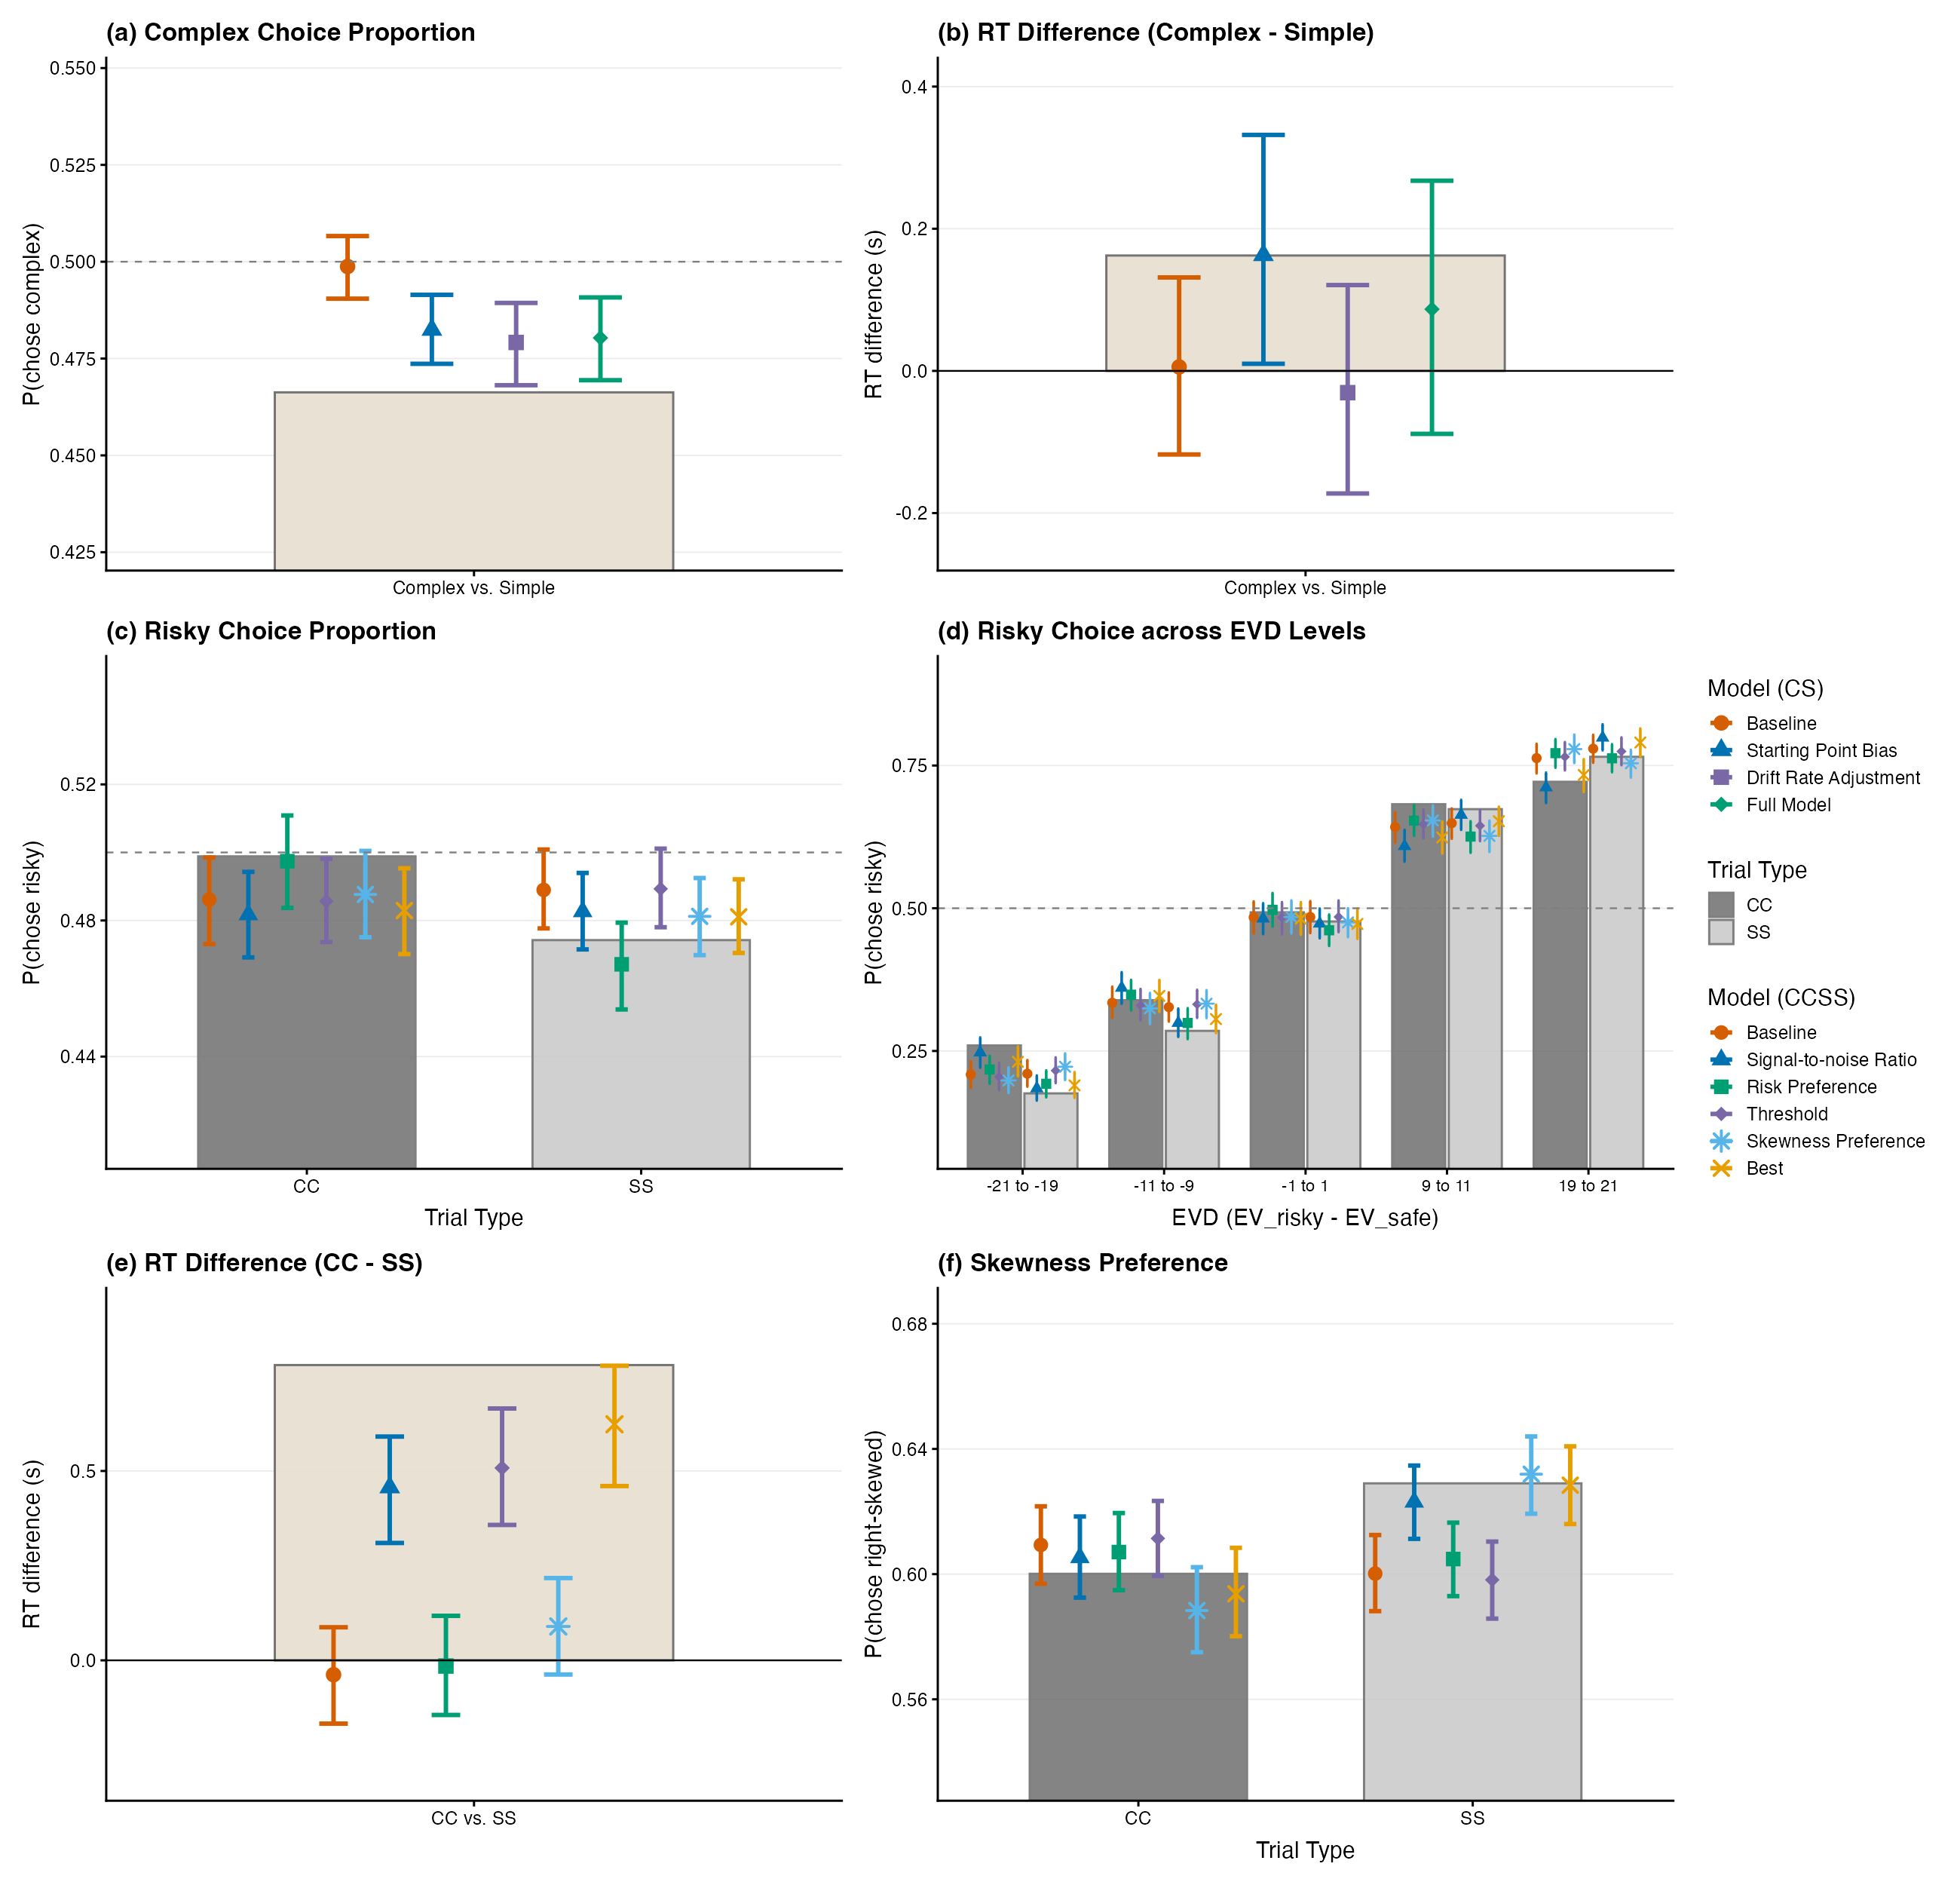
\includegraphics[width=\textwidth]{figures/ppc_cpt_study1.png}
    \caption{Posterior predictive checks for the CPT-based models, Study~1. Grey/beige bars are observed data; coloured points are posterior predictive means with 95\% credible intervals (1{,}600 draws). Panels (a, b) summarise the CS condition; panels (c--f) summarise the CCSS condition. The best-fitting CPT model under the parsimony rule (see the §CPT-Based Model Results section above) is shown as ``Best'' (gold).}
    \label{fig:ppc_cpt_study1}
\end{figure}

\begin{figure}[!htbp]
    \centering
    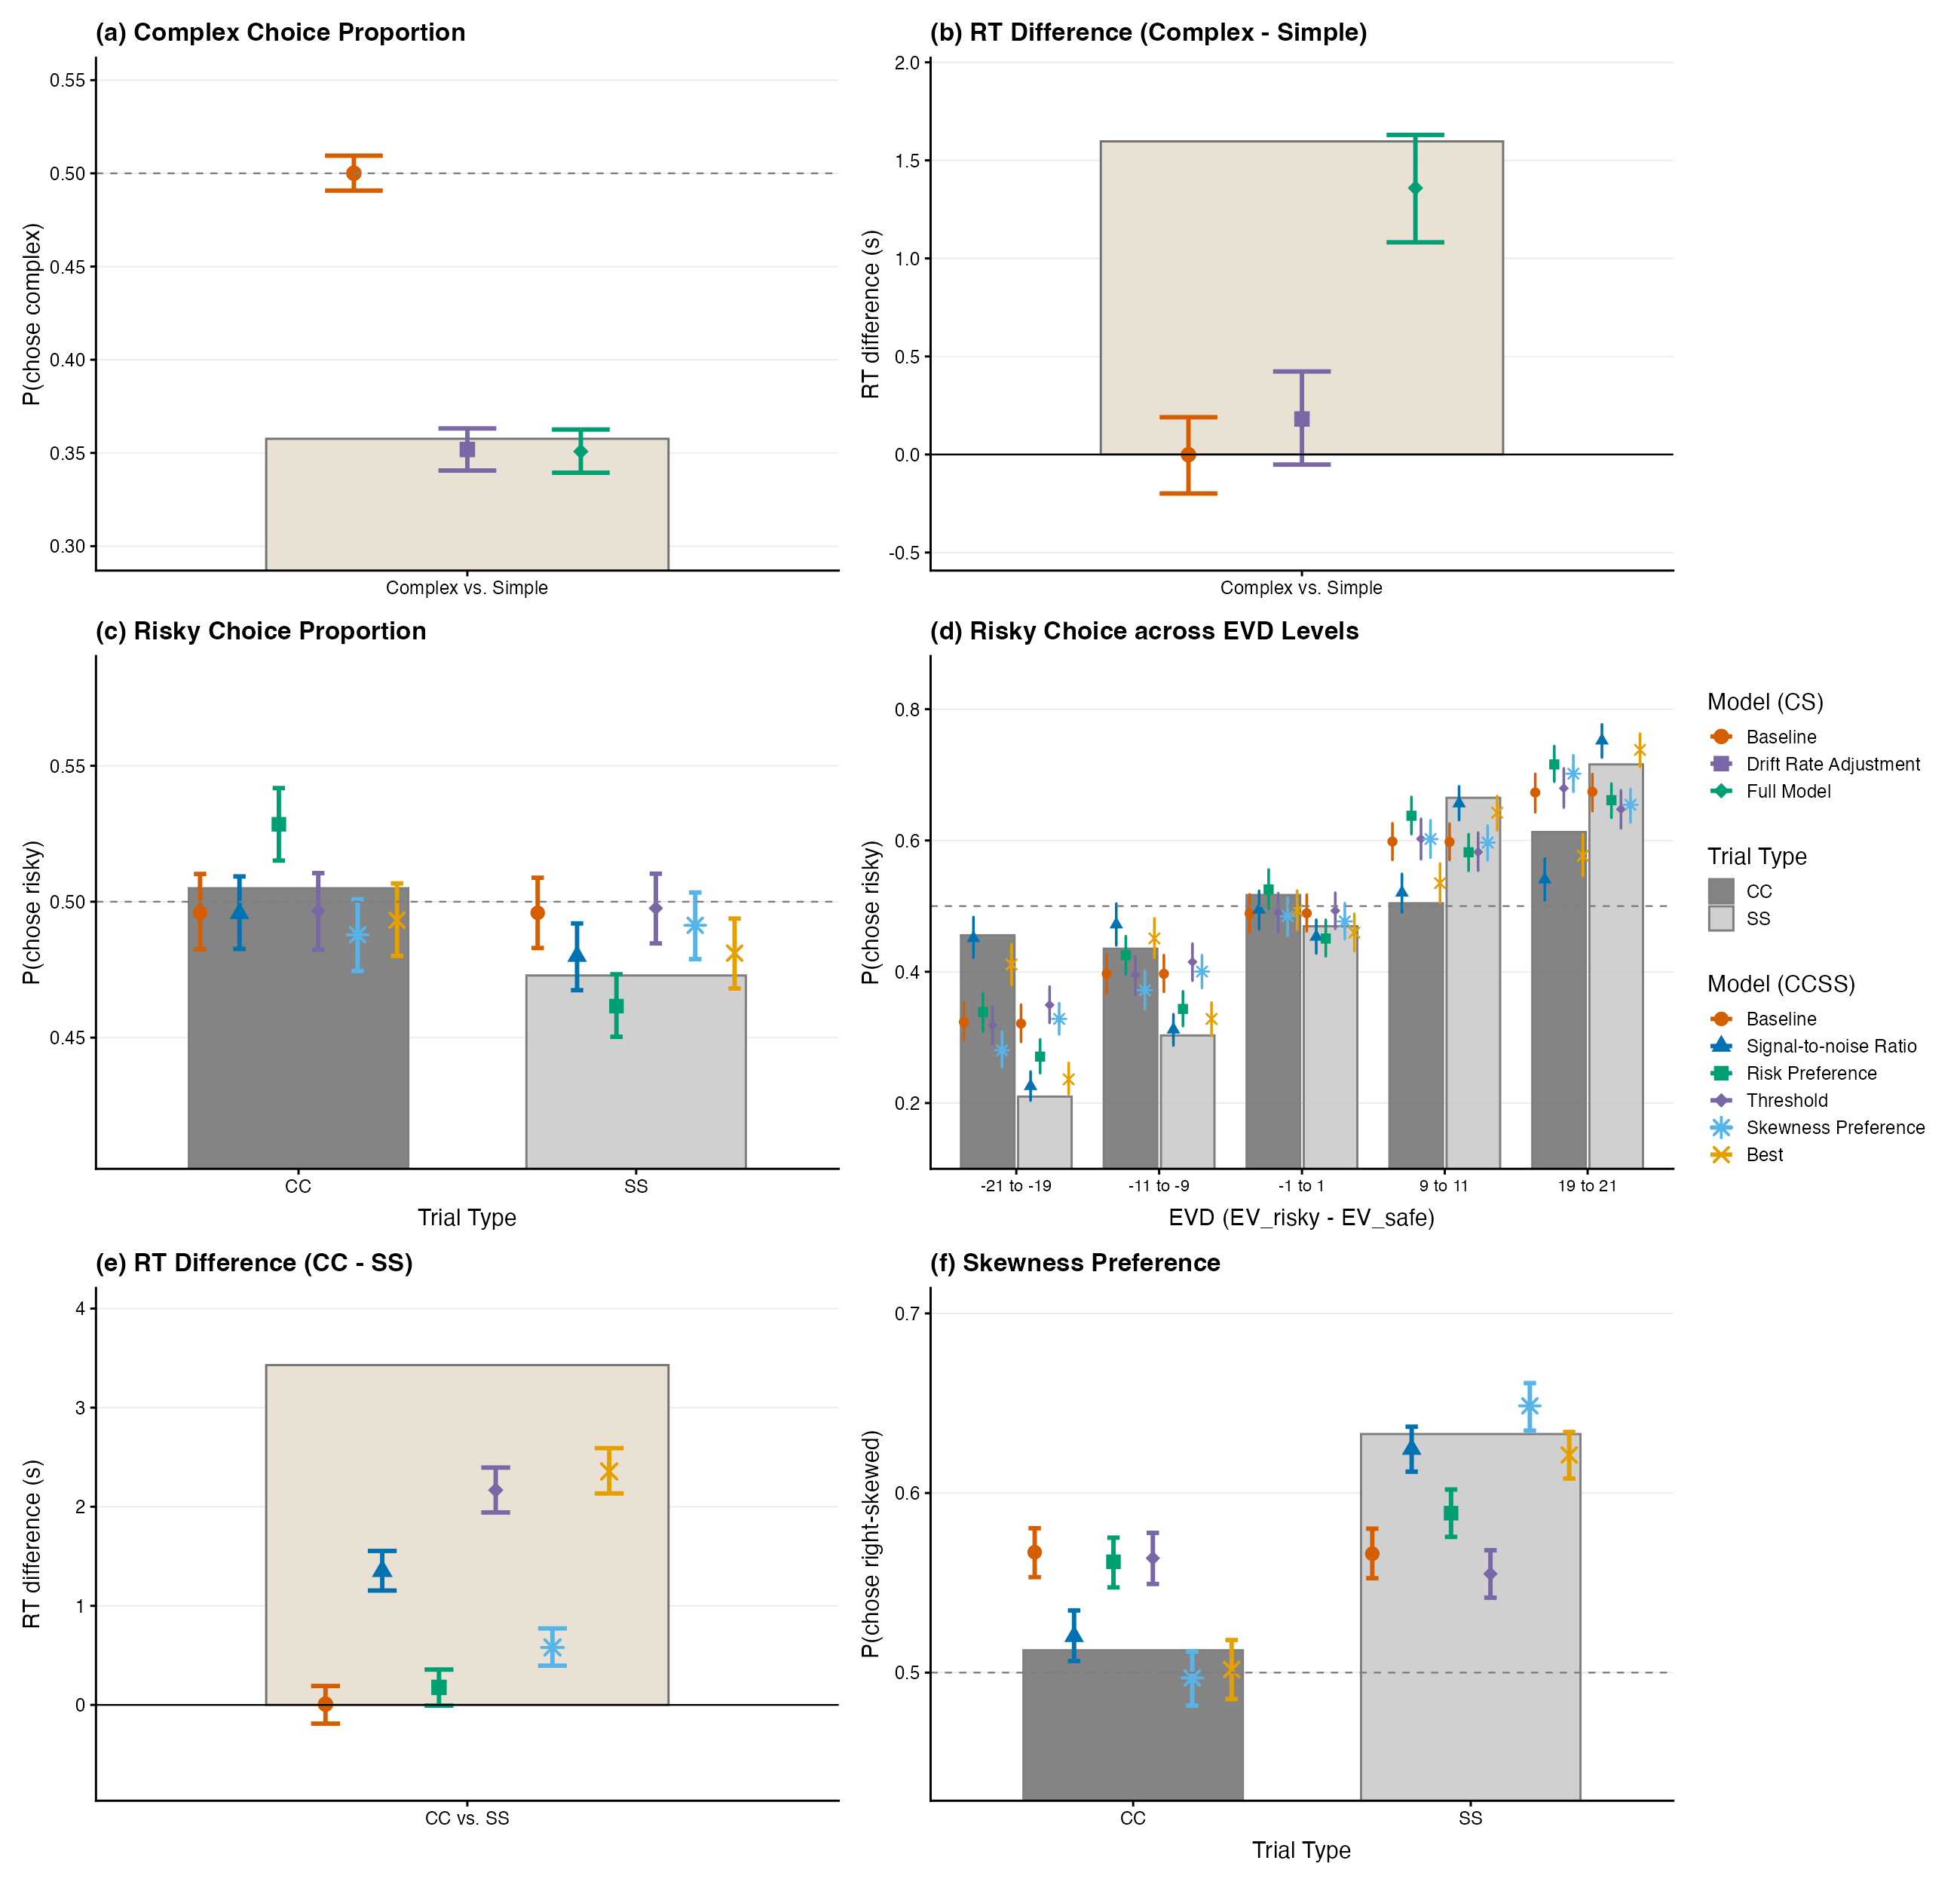
\includegraphics[width=\textwidth]{figures/ppc_cpt_study2.png}
    \caption{Posterior predictive checks for the CPT-based models, Study~2. Conventions as in Figure~\ref{fig:ppc_cpt_study1}.}
    \label{fig:ppc_cpt_study2}
\end{figure}

\begin{figure}[!htbp]
    \centering
    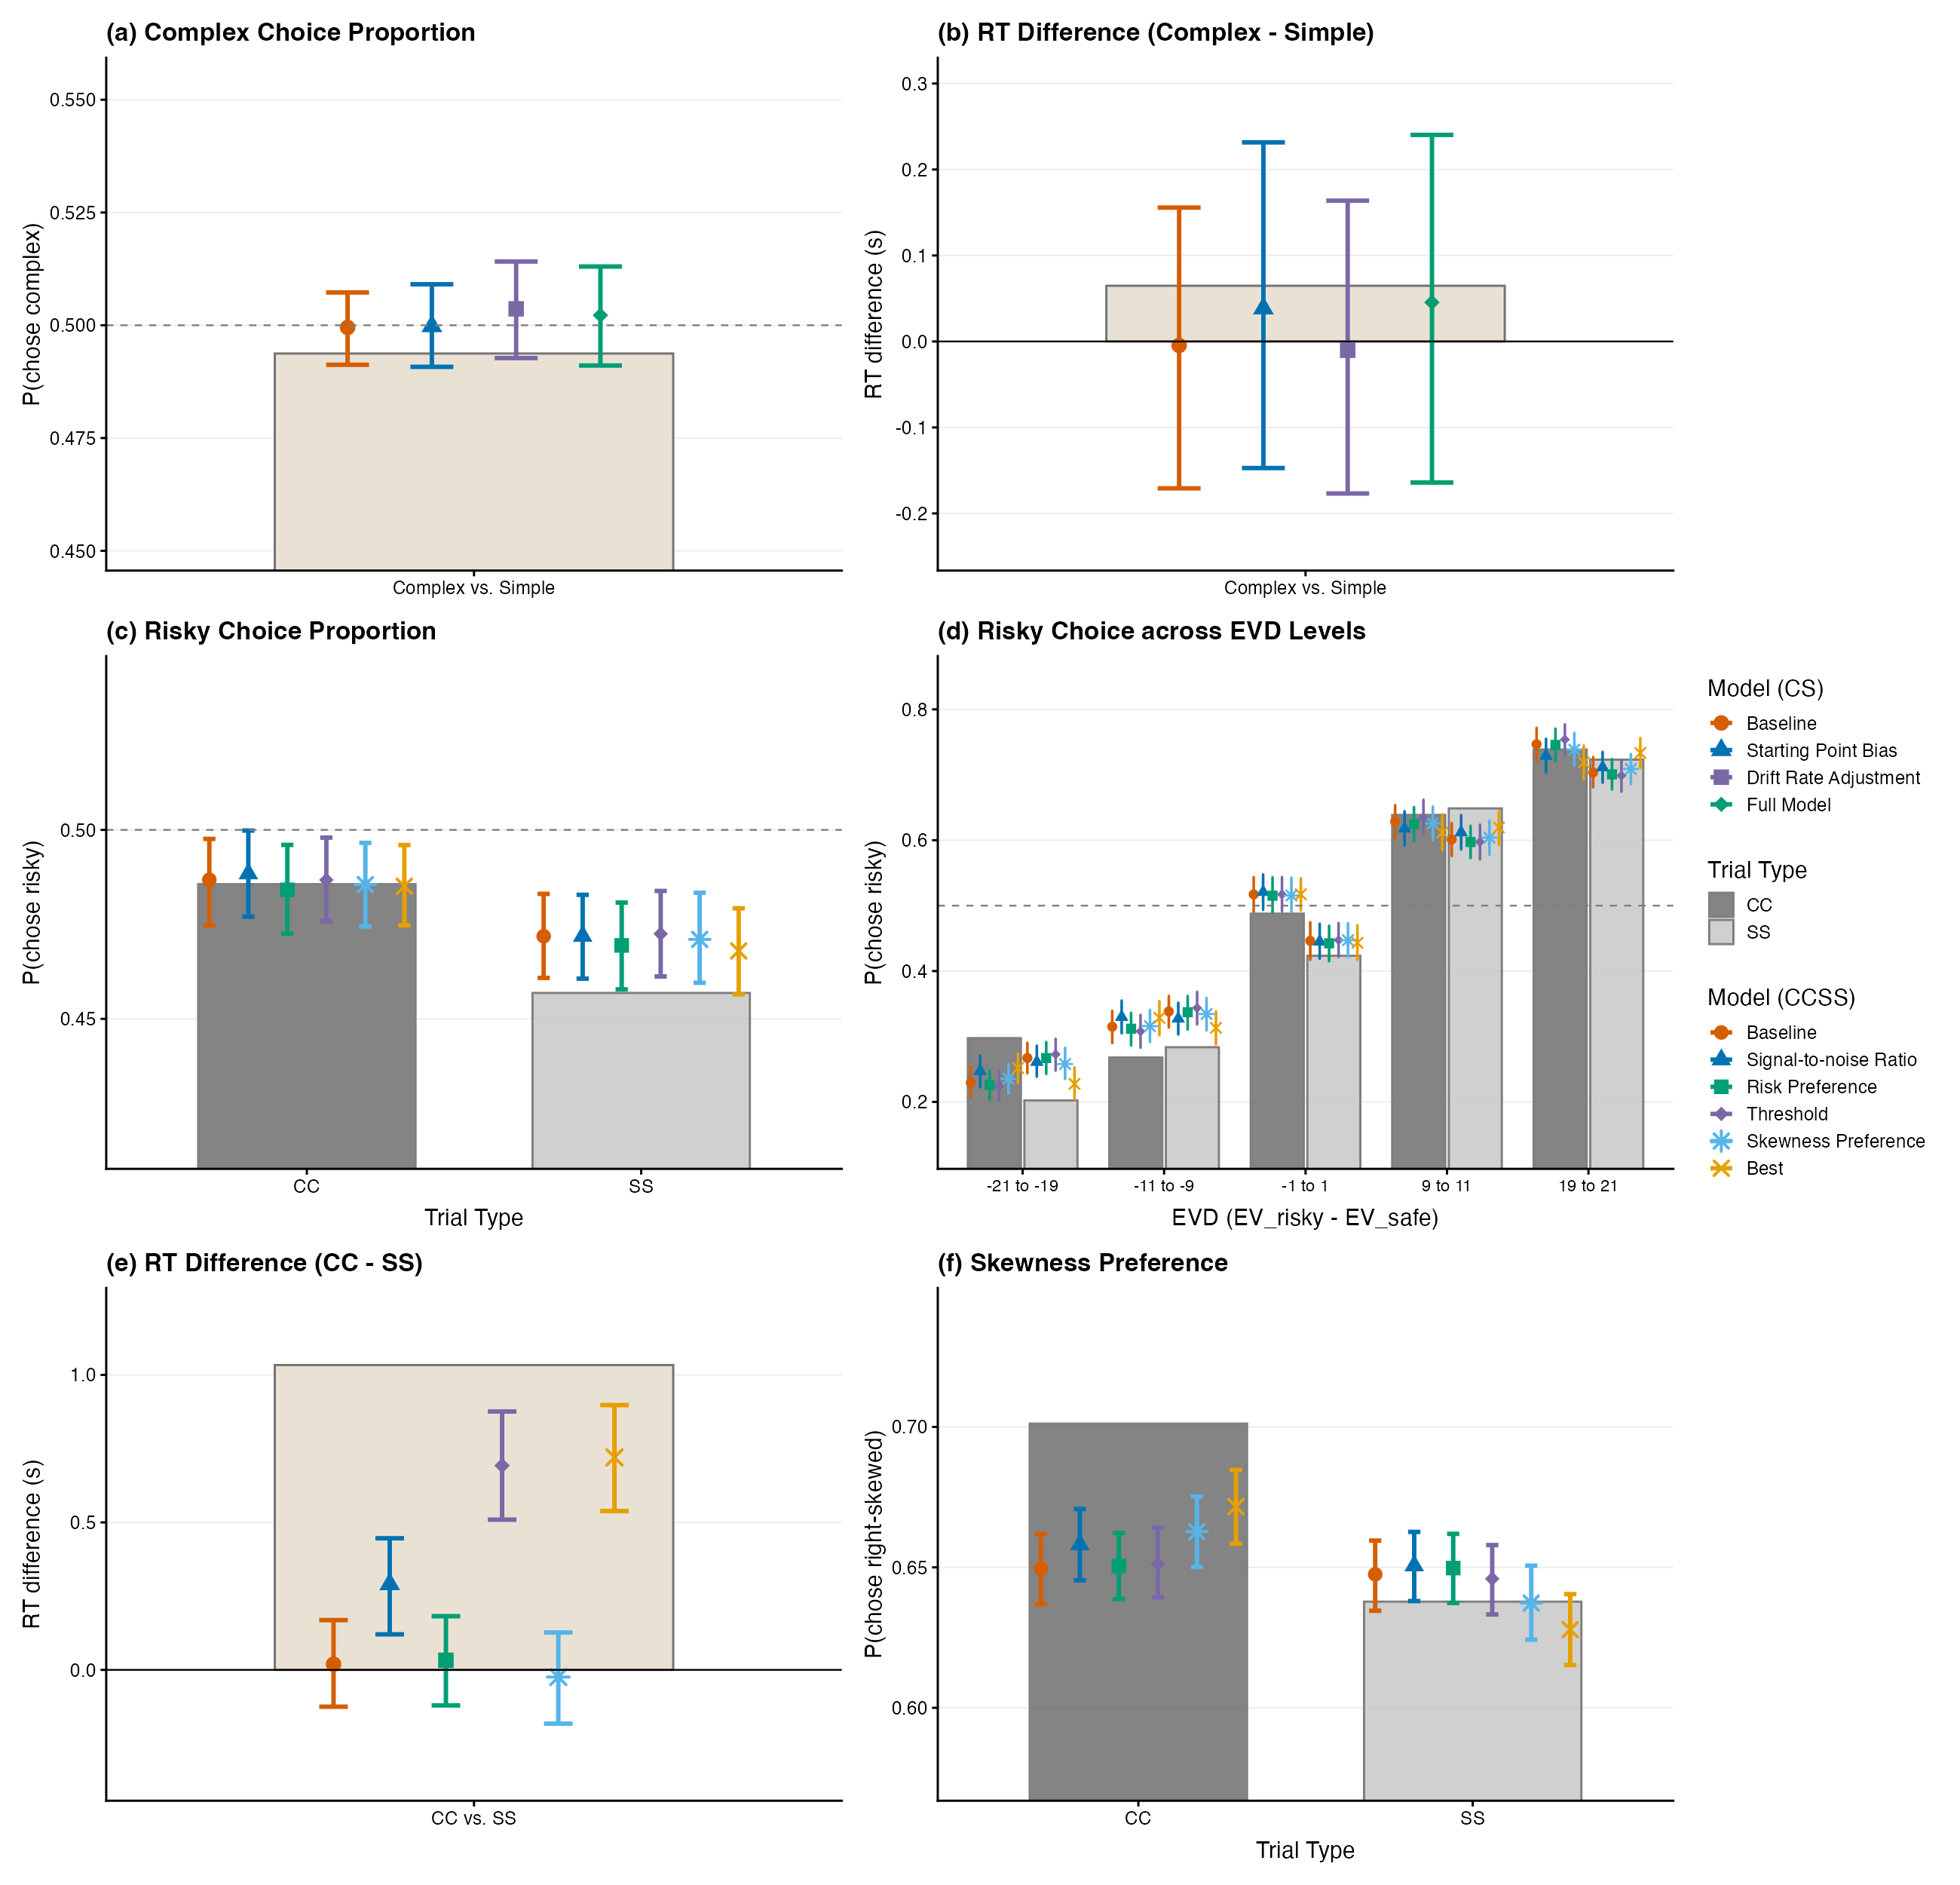
\includegraphics[width=\textwidth]{figures/ppc_cpt_study3.png}
    \caption{Posterior predictive checks for the CPT-based models, Study~3. Conventions as in Figure~\ref{fig:ppc_cpt_study1}.}
    \label{fig:ppc_cpt_study3}
\end{figure}

\subsection{Individual-Level Posterior Predictive Checks}

To confirm that the CPT-based models capture individual heterogeneity as well as the MVS models do in the main text, we repeated the individual-level PPCs for the CPT family using the same procedures as in the Appendix. For the CS condition we compared each participant's observed and predicted complex-choice proportion and median RT difference (choosing complex minus simple). For the CCSS condition we compared each participant's observed and predicted median CC$-$SS RT difference and their EV-consistency effect, the latter indexed by the EVD $\times$ complexity interaction coefficient from a per-participant generalized linear model (the model-free proxy for the signal-to-noise ratio). Across all three studies the pattern mirrors the MVS results: the baseline CPT model fails to reproduce the individual-level effects, whereas the parsimonious best model recovers the observed distribution of individual choice and RT differences (Figures~\ref{fig:ppc_cpt_ind_s1_cschoice}--\ref{fig:ppc_cpt_ind_s3_ccssrt}).

%% ---- Study 1 ----
\begin{figure}[!htbp]
    \caption{Individual-level posterior predictive check of complex-choice proportion in the CS condition of Study~1 (CPT-based models)}
    \begin{center}
        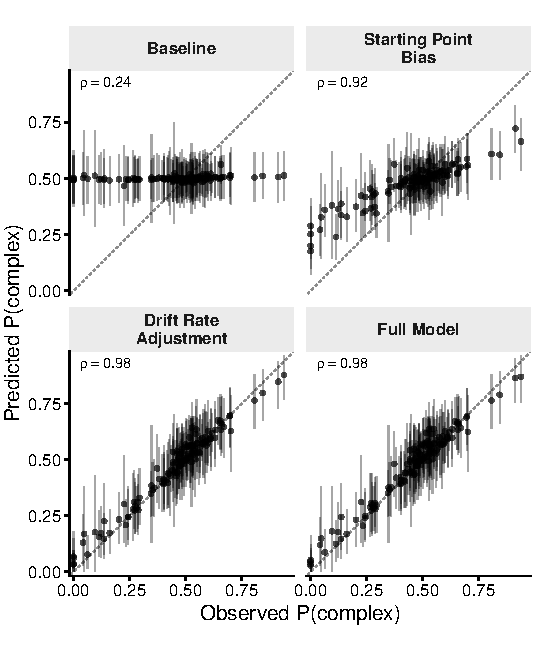
\includegraphics[width=0.8\textwidth, keepaspectratio]{figures/ppc_cpt_ind_study1_cs_complex_choice.pdf}
    \end{center}
    \label{fig:ppc_cpt_ind_s1_cschoice}
    \textit{Note.} Each panel is one CPT model. The $x$-axis is each participant's observed proportion of complex choices; the $y$-axis is the corresponding proportion from that model's posterior predictive simulations. The dashed diagonal marks perfect prediction.
\end{figure}

\begin{figure}[!htbp]
    \caption{Individual-level posterior predictive check of RT difference in the CS condition of Study~1 (CPT-based models)}
    \begin{center}
        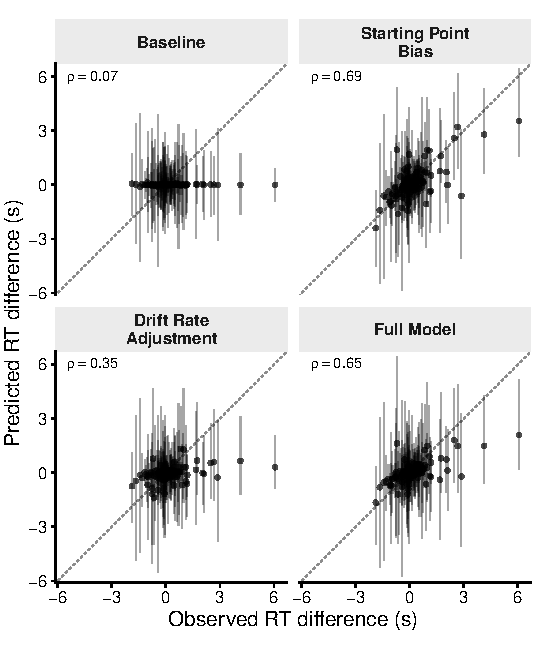
\includegraphics[width=0.8\textwidth, keepaspectratio]{figures/ppc_cpt_ind_study1_cs_rt_diff.pdf}
    \end{center}
    \label{fig:ppc_cpt_ind_s1_csrt}
    \textit{Note.} The $x$-axis is each participant's observed RT difference (choosing complex minus simple); the $y$-axis is the corresponding predicted difference from each model's posterior simulations. The dashed diagonal marks perfect prediction.
\end{figure}

\begin{figure}[!htbp]
    \caption{Individual-level posterior predictive check of EV consistency in the CCSS condition of Study~1 (CPT-based models)}
    \begin{center}
        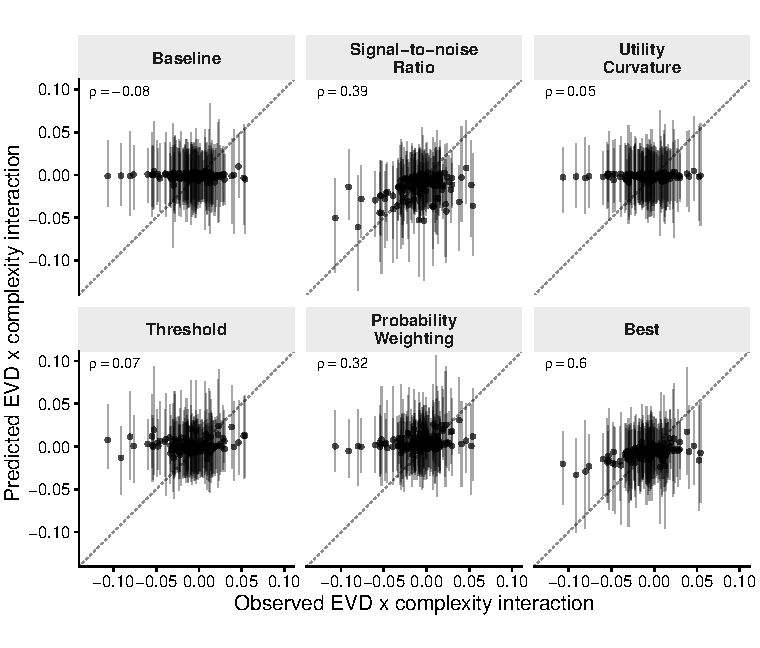
\includegraphics[width=\textwidth]{figures/ppc_cpt_ind_study1_ccss_consistency.pdf}
    \end{center}
    \label{fig:ppc_cpt_ind_s1_ccsscons}
    \textit{Note.} The $x$-axis is each participant's observed EVD $\times$ complexity interaction coefficient (the model-free SNR proxy); the $y$-axis is the corresponding coefficient computed from each model's predicted choices. The dashed diagonal marks perfect prediction.
\end{figure}

\begin{figure}[!htbp]
    \caption{Individual-level posterior predictive check of RT difference in the CCSS condition of Study~1 (CPT-based models)}
    \begin{center}
        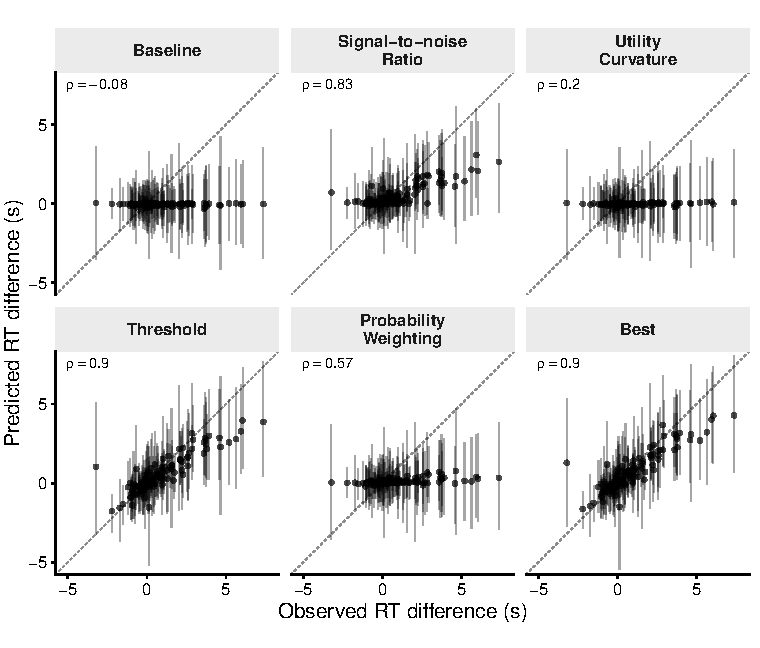
\includegraphics[width=\textwidth]{figures/ppc_cpt_ind_study1_ccss_rt_diff.pdf}
    \end{center}
    \label{fig:ppc_cpt_ind_s1_ccssrt}
    \textit{Note.} The $x$-axis is each participant's observed median CC$-$SS RT difference; the $y$-axis is the corresponding predicted difference from each model. The dashed diagonal marks perfect prediction.
\end{figure}

%% ---- Study 2 ----
\begin{figure}[!htbp]
    \caption{Individual-level posterior predictive check of complex-choice proportion in the CS condition of Study~2 (CPT-based models)}
    \begin{center}
        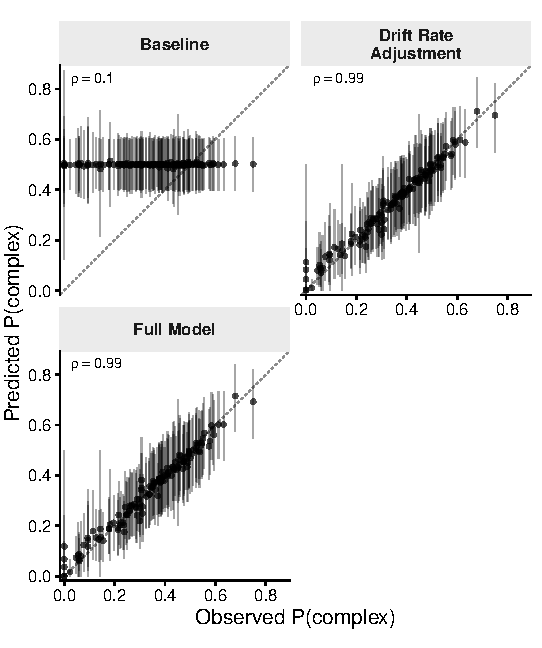
\includegraphics[width=0.8\textwidth, keepaspectratio]{figures/ppc_cpt_ind_study2_cs_complex_choice.pdf}
    \end{center}
    \label{fig:ppc_cpt_ind_s2_cschoice}
    \textit{Note.} Conventions as in Figure~\ref{fig:ppc_cpt_ind_s1_cschoice}.
\end{figure}

\begin{figure}[!htbp]
    \caption{Individual-level posterior predictive check of RT difference in the CS condition of Study~2 (CPT-based models)}
    \begin{center}
        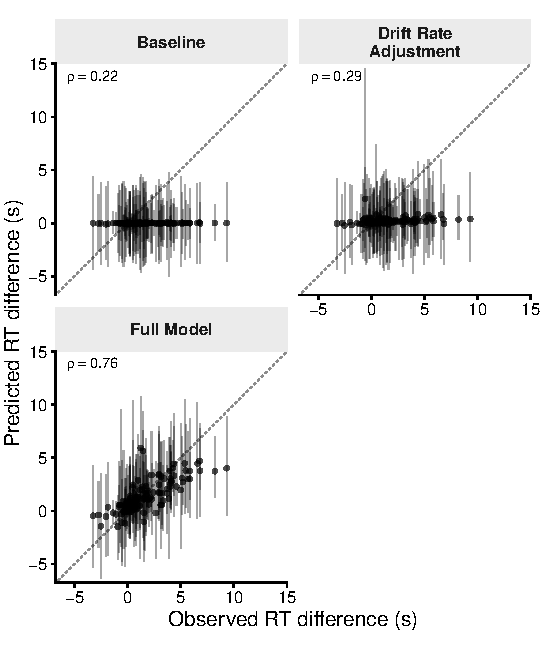
\includegraphics[width=0.8\textwidth, keepaspectratio]{figures/ppc_cpt_ind_study2_cs_rt_diff.pdf}
    \end{center}
    \label{fig:ppc_cpt_ind_s2_csrt}
    \textit{Note.} Conventions as in Figure~\ref{fig:ppc_cpt_ind_s1_csrt}.
\end{figure}

\begin{figure}[!htbp]
    \caption{Individual-level posterior predictive check of EV consistency in the CCSS condition of Study~2 (CPT-based models)}
    \begin{center}
        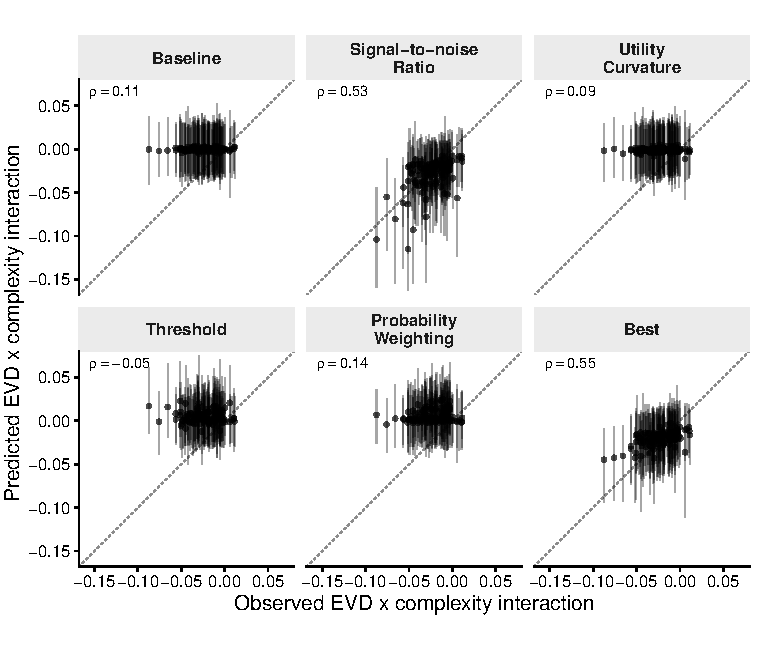
\includegraphics[width=\textwidth]{figures/ppc_cpt_ind_study2_ccss_consistency.pdf}
    \end{center}
    \label{fig:ppc_cpt_ind_s2_ccsscons}
    \textit{Note.} Conventions as in Figure~\ref{fig:ppc_cpt_ind_s1_ccsscons}.
\end{figure}

\begin{figure}[!htbp]
    \caption{Individual-level posterior predictive check of RT difference in the CCSS condition of Study~2 (CPT-based models)}
    \begin{center}
        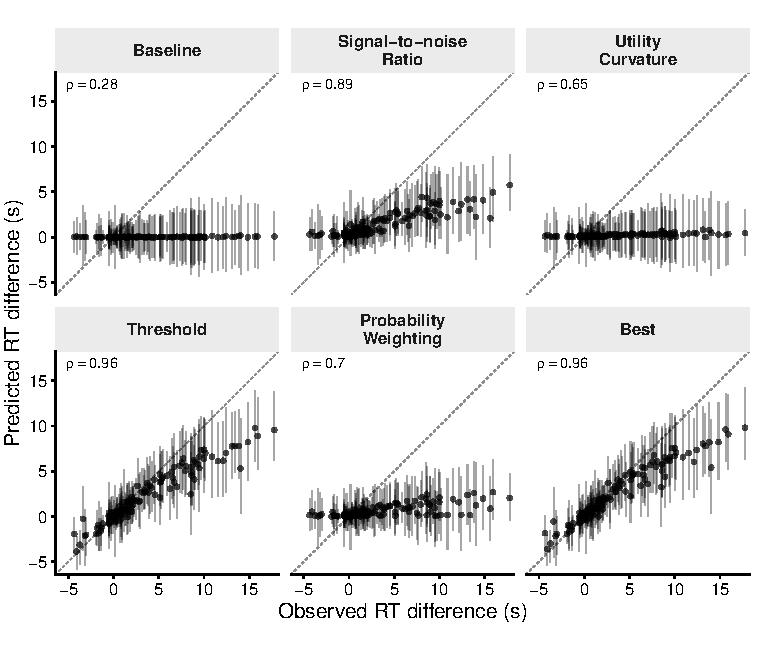
\includegraphics[width=\textwidth]{figures/ppc_cpt_ind_study2_ccss_rt_diff.pdf}
    \end{center}
    \label{fig:ppc_cpt_ind_s2_ccssrt}
    \textit{Note.} Conventions as in Figure~\ref{fig:ppc_cpt_ind_s1_ccssrt}.
\end{figure}

%% ---- Study 3 ----
\begin{figure}[!htbp]
    \caption{Individual-level posterior predictive check of complex-choice proportion in the CS condition of Study~3 (CPT-based models)}
    \begin{center}
        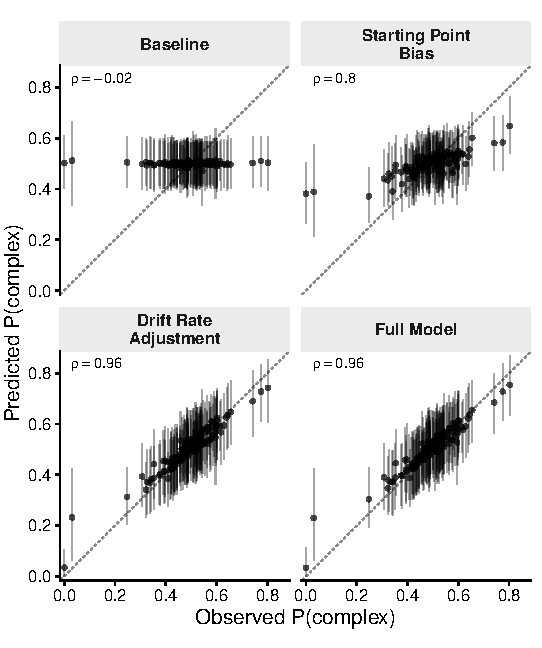
\includegraphics[width=0.8\textwidth, keepaspectratio]{figures/ppc_cpt_ind_study3_cs_complex_choice.pdf}
    \end{center}
    \label{fig:ppc_cpt_ind_s3_cschoice}
    \textit{Note.} Conventions as in Figure~\ref{fig:ppc_cpt_ind_s1_cschoice}.
\end{figure}

\begin{figure}[!htbp]
    \caption{Individual-level posterior predictive check of RT difference in the CS condition of Study~3 (CPT-based models)}
    \begin{center}
        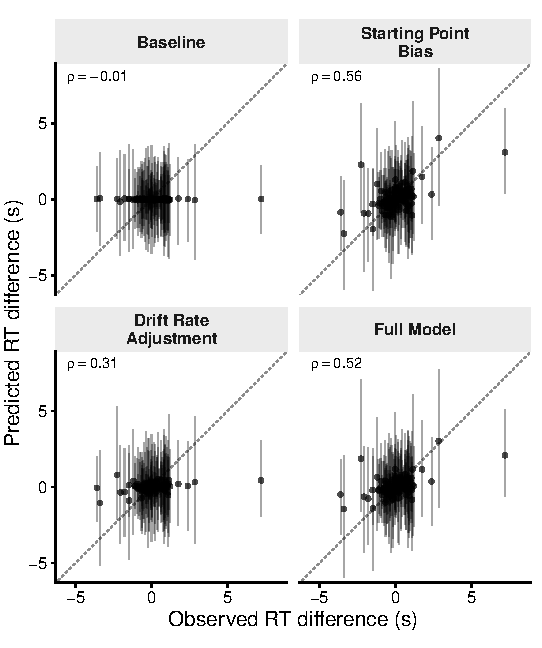
\includegraphics[width=0.8\textwidth, keepaspectratio]{figures/ppc_cpt_ind_study3_cs_rt_diff.pdf}
    \end{center}
    \label{fig:ppc_cpt_ind_s3_csrt}
    \textit{Note.} Conventions as in Figure~\ref{fig:ppc_cpt_ind_s1_csrt}.
\end{figure}

\begin{figure}[!htbp]
    \caption{Individual-level posterior predictive check of EV consistency in the CCSS condition of Study~3 (CPT-based models)}
    \begin{center}
        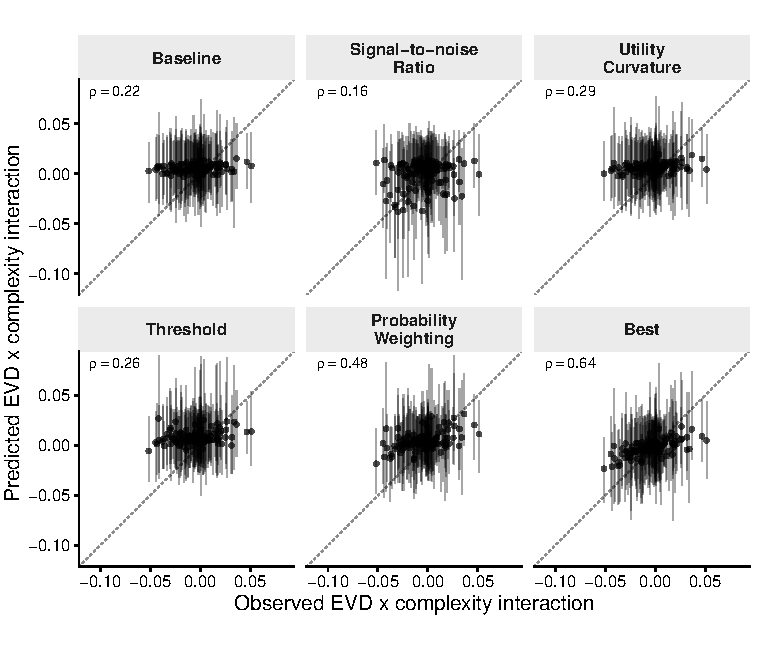
\includegraphics[width=\textwidth]{figures/ppc_cpt_ind_study3_ccss_consistency.pdf}
    \end{center}
    \label{fig:ppc_cpt_ind_s3_ccsscons}
    \textit{Note.} Conventions as in Figure~\ref{fig:ppc_cpt_ind_s1_ccsscons}.
\end{figure}

\begin{figure}[!htbp]
    \caption{Individual-level posterior predictive check of RT difference in the CCSS condition of Study~3 (CPT-based models)}
    \begin{center}
        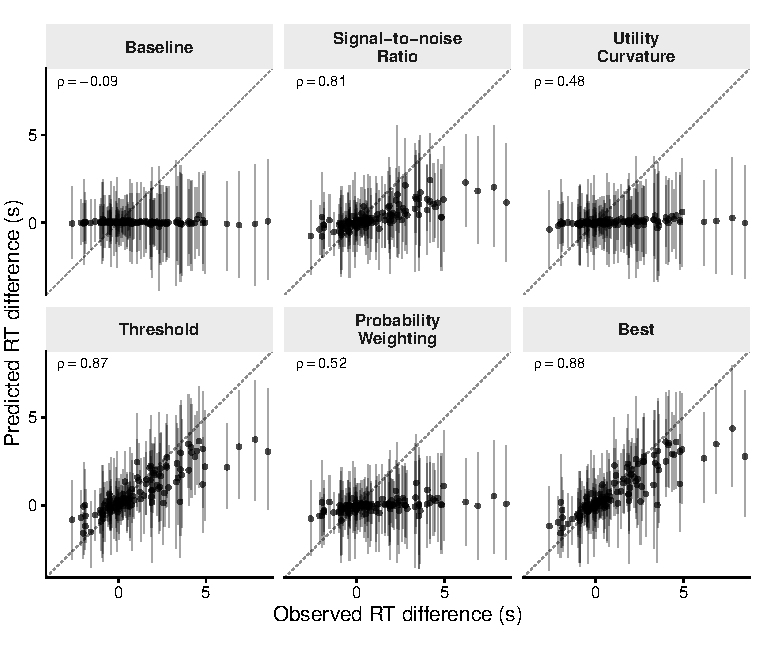
\includegraphics[width=\textwidth]{figures/ppc_cpt_ind_study3_ccss_rt_diff.pdf}
    \end{center}
    \label{fig:ppc_cpt_ind_s3_ccssrt}
    \textit{Note.} Conventions as in Figure~\ref{fig:ppc_cpt_ind_s1_ccssrt}.
\end{figure}

\FloatBarrier

%% ============================================================================
\section{A Preregistered Mechanism Excluded from Model Comparison: Differential Skewness Sensitivity}
\label{sec:skew_diff}
%% ============================================================================

Alongside the starting-point bias ($z$) and the drift-rate adjustment ($\zeta$), we preregistered a third candidate mechanism for the CS condition: a differential sensitivity to skewness---in the CPT representation, to probability weighting---for complex versus simple options (Hypothesis~2.3: a credible difference in the processing of the complex and simple option, with the 95\% highest-posterior-density interval (HPDI) of the difference parameter excluding zero). The idea was that participants might weight the skewness of the complex and simple options to different degrees, showing heightened skewness sensitivity for the complex option and reduced sensitivity for the simple one.

In the MVS representation this is captured by splitting the single skewness weight $\eta$ into option-specific weights governed by a difference parameter $\Delta_\eta$ (here the within-trial complex-vs-simple skewness-weight difference in the CS condition, not to be confused with the CCSS skewness-preference shift of the same name):
\begin{equation}
v \;=\; \theta \cdot \Bigl(\text{EVD} + \beta \cdot \text{SDD} + (\eta + \Delta_\eta)\,\text{skew}_{\text{c}} - (\eta - \Delta_\eta)\,\text{skew}_{\text{s}} \Bigr),
\end{equation}
where $\text{skew}_{\text{c}}$ and $\text{skew}_{\text{s}}$ are the skewness of the complex and simple option, a positive $\Delta_\eta$ denotes stronger skewness sensitivity for the complex option, and $\Delta_\eta = 0$ recovers the baseline. The CPT representation implements the same idea on the Prelec curvature $\gamma$ via an analogous difference parameter $\Delta_\gamma$.

We excluded this mechanism from the main model comparison because it produces no observable behavioural signature under our fully balanced design. In a simulation using the 90 CS-condition trials replicated 500 times, we set $\eta = 2$ and $\Delta_\eta = 4$---extreme option-specific sensitivities of $+6$ (complex) and $-2$ (simple)---yet the simulated complex-choice proportion was virtually identical to that of the baseline model (0.4985 vs.\ 0.4991). The reason is the trial structure: one third of the complex options were right-skewed, one third left-skewed, and one third symmetric, so a constant difference in skewness sensitivity cancels at the aggregate level regardless of its magnitude.


%% ============================================================================
\section{Response-Time Distribution Fit}
\label{sec:rtdist}
%% ============================================================================

A standard validation for evidence-accumulation models is whether the fitted model reproduces the full \emph{shape} of the empirical response-time (RT) distribution, not only summary statistics. Figures~\ref{fig:rtdist_study1}--\ref{fig:rtdist_study3} overlay the observed RT distributions (histograms) with the posterior-predictive RT densities (curves) of the best-fitting model in each condition, separately for the MVS (main-text) and CPT (robustness) value representations and for the CS and CCSS conditions, split by the chosen option. Across all studies, conditions, and both value representations, the predicted densities closely track the observed distributions---including the pronounced right skew and the separation between response types---confirming that the models capture the timing of choices as well as their proportions.

\begin{figure}[!htbp]
\caption{Empirical vs.\ Posterior-Predicted RT Distributions for the Best-Fitting Models, Study~1}
\label{fig:rtdist_study1}
\centering
\begin{minipage}{0.49\textwidth}\centering
  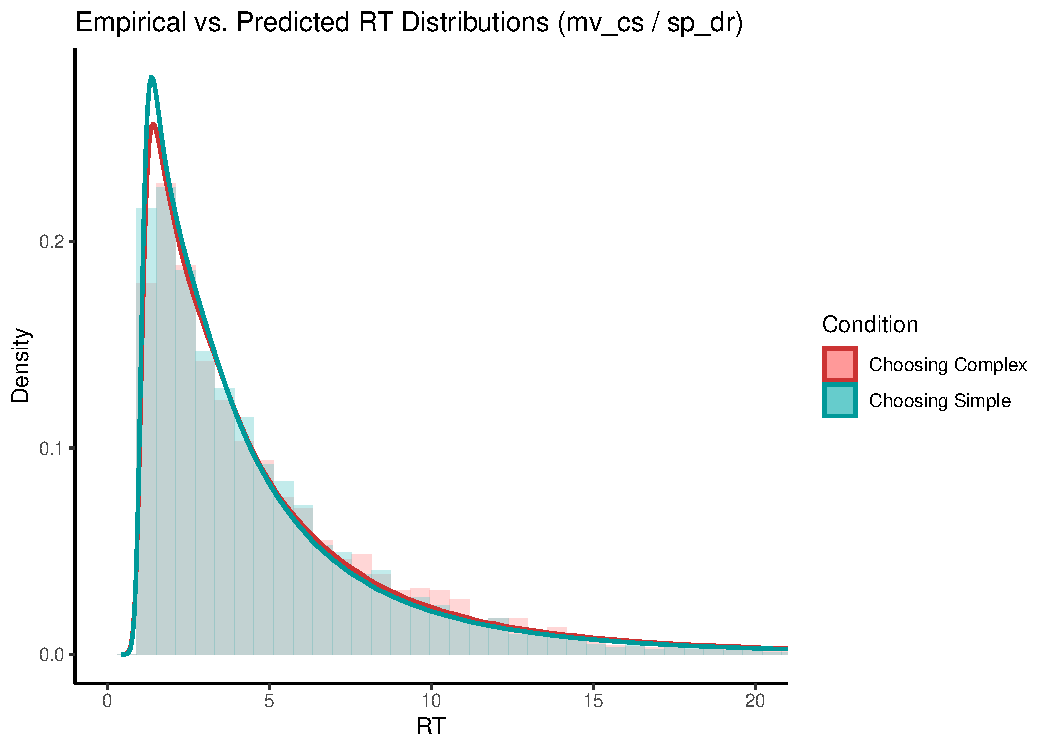
\includegraphics[width=\linewidth]{figures/ppc_rtdist_mv_cs_study1.pdf}\\[-2pt]{\footnotesize (a) MVS --- CS condition}\end{minipage}\hfill
\begin{minipage}{0.49\textwidth}\centering
  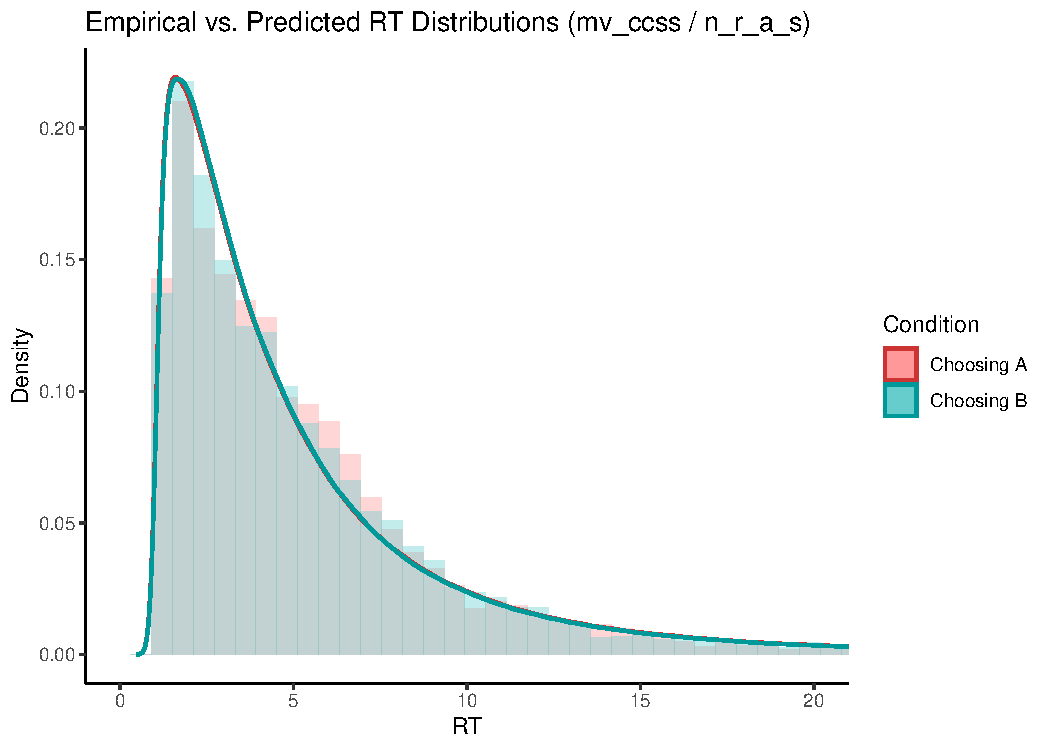
\includegraphics[width=\linewidth]{figures/ppc_rtdist_mv_ccss_study1.pdf}\\[-2pt]{\footnotesize (b) MVS --- CCSS condition}\end{minipage}

\vspace{4pt}
\begin{minipage}{0.49\textwidth}\centering
  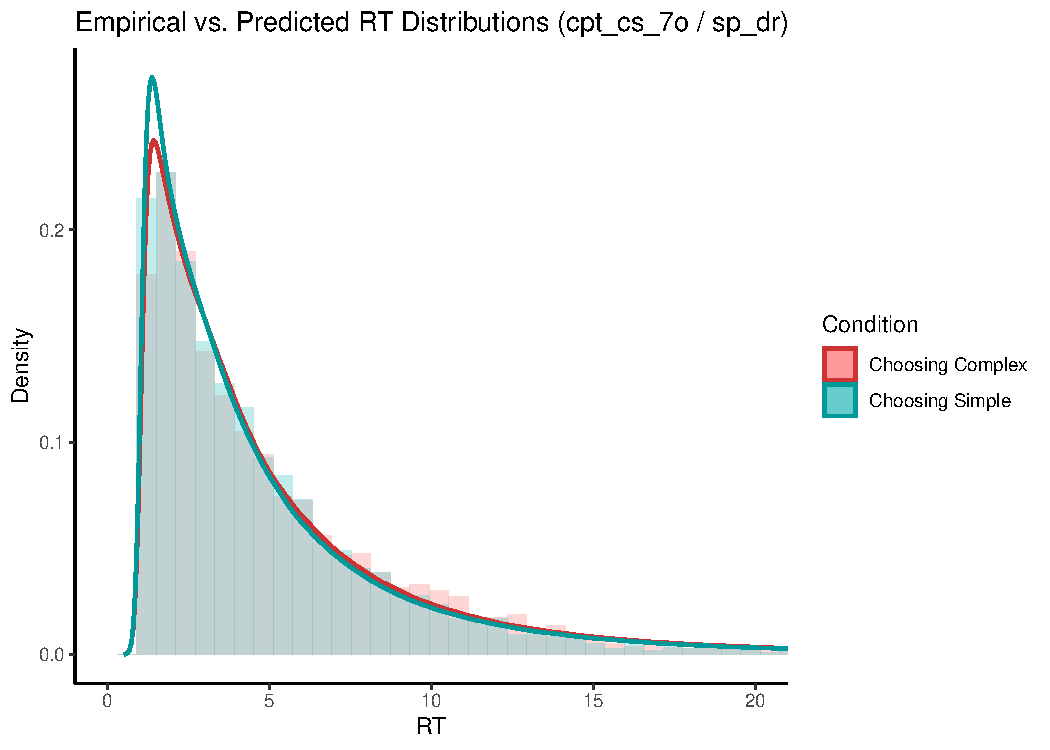
\includegraphics[width=\linewidth]{figures/ppc_rtdist_cpt_cs_study1.pdf}\\[-2pt]{\footnotesize (c) CPT --- CS condition}\end{minipage}\hfill
\begin{minipage}{0.49\textwidth}\centering
  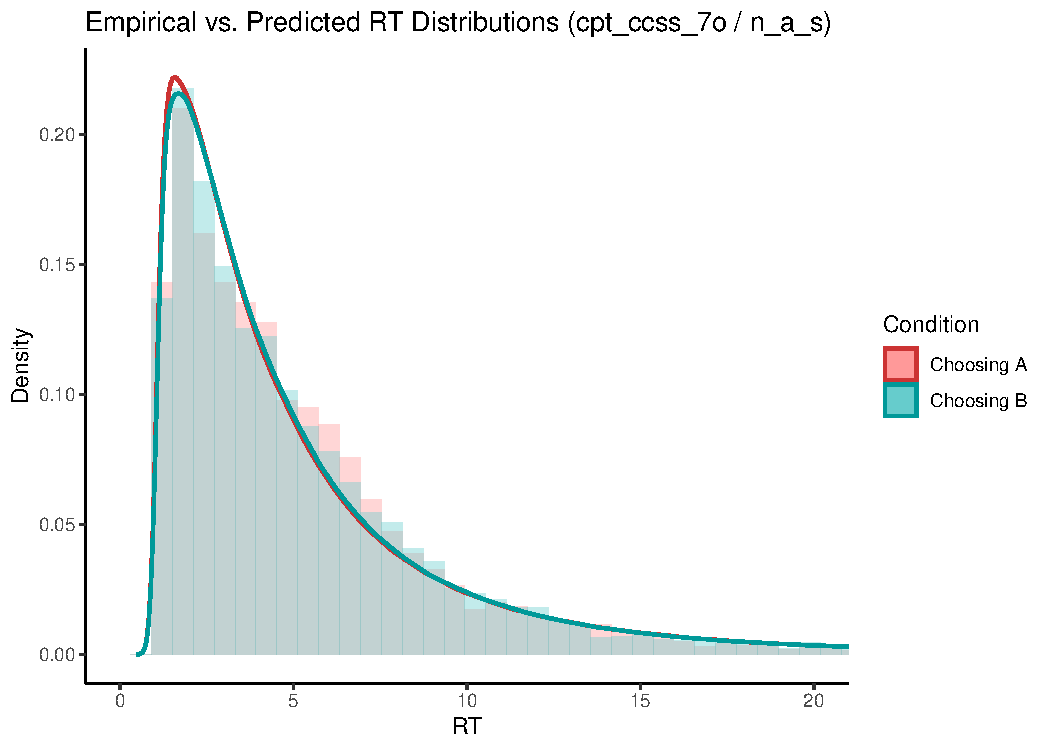
\includegraphics[width=\linewidth]{figures/ppc_rtdist_cpt_ccss_study1.pdf}\\[-2pt]{\footnotesize (d) CPT --- CCSS condition}\end{minipage}

\vspace{2pt}
\raggedright\textit{Note.} Histograms are observed RTs; curves are posterior-predictive densities from the best-fitting model, split by the chosen option. Panels: (a) MVS CS; (b) MVS CCSS; (c) CPT CS; (d) CPT CCSS. RTs are in seconds; the horizontal axis is truncated at 20~s.
\end{figure}

\begin{figure}[!htbp]
\caption{Empirical vs.\ Posterior-Predicted RT Distributions for the Best-Fitting Models, Study~2}
\label{fig:rtdist_study2}
\centering
\begin{minipage}{0.49\textwidth}\centering
  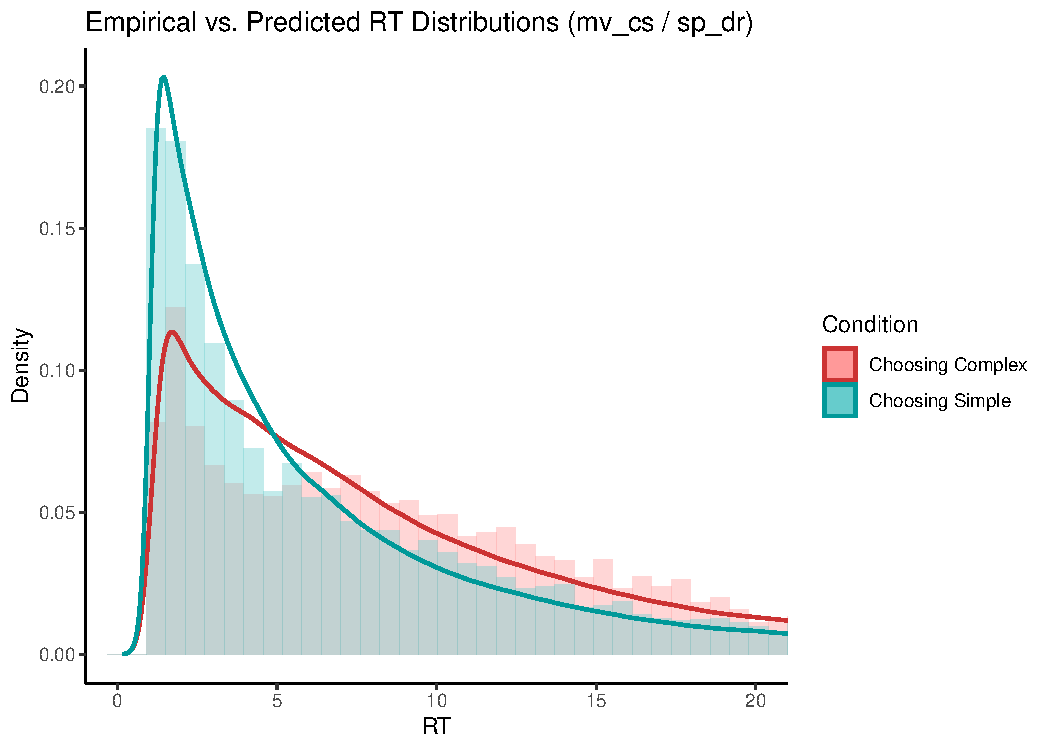
\includegraphics[width=\linewidth]{figures/ppc_rtdist_mv_cs_study2.pdf}\\[-2pt]{\footnotesize (a) MVS --- CS condition}\end{minipage}\hfill
\begin{minipage}{0.49\textwidth}\centering
  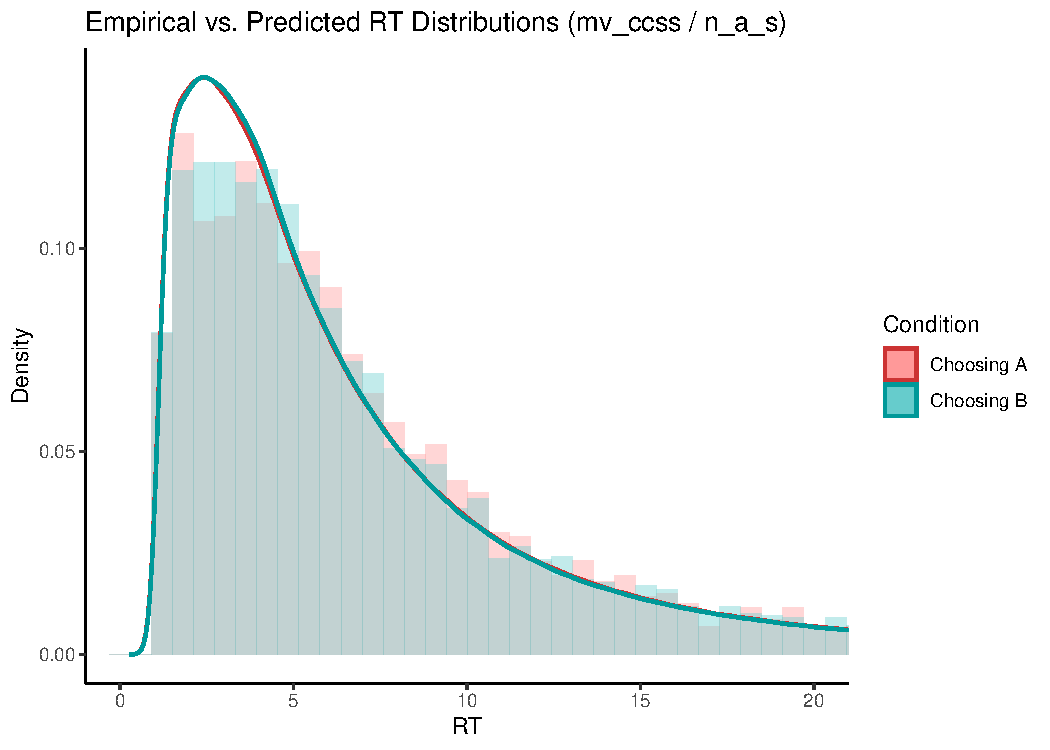
\includegraphics[width=\linewidth]{figures/ppc_rtdist_mv_ccss_study2.pdf}\\[-2pt]{\footnotesize (b) MVS --- CCSS condition}\end{minipage}

\vspace{4pt}
\begin{minipage}{0.49\textwidth}\centering
  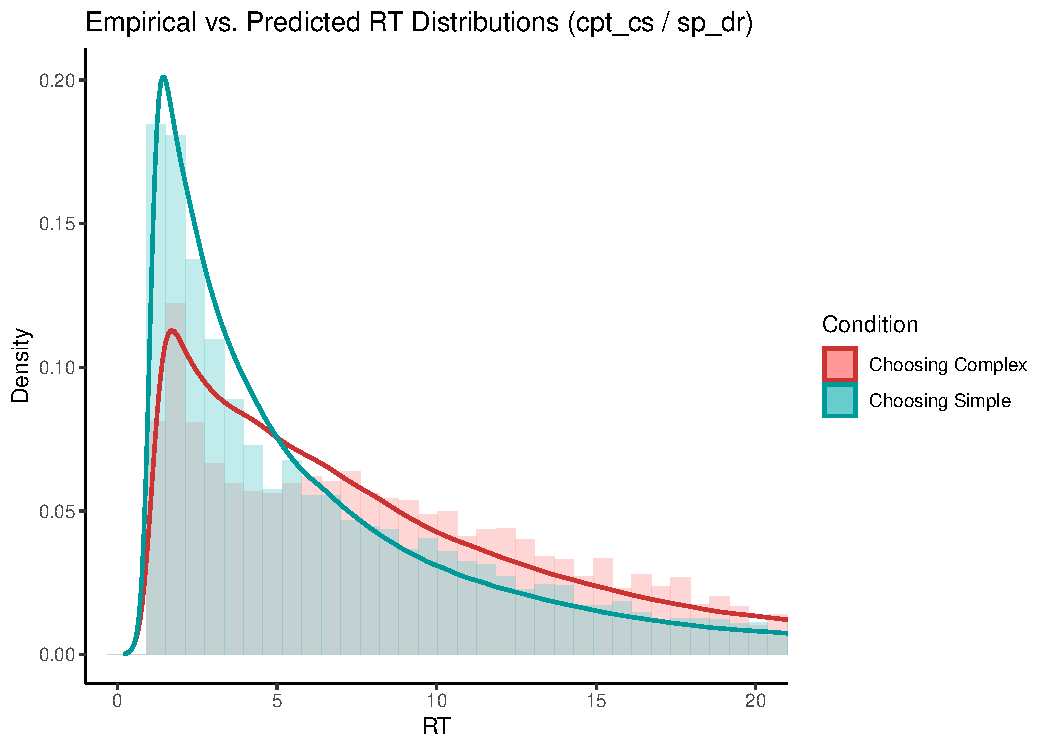
\includegraphics[width=\linewidth]{figures/ppc_rtdist_cpt_cs_study2.pdf}\\[-2pt]{\footnotesize (c) CPT --- CS condition}\end{minipage}\hfill
\begin{minipage}{0.49\textwidth}\centering
  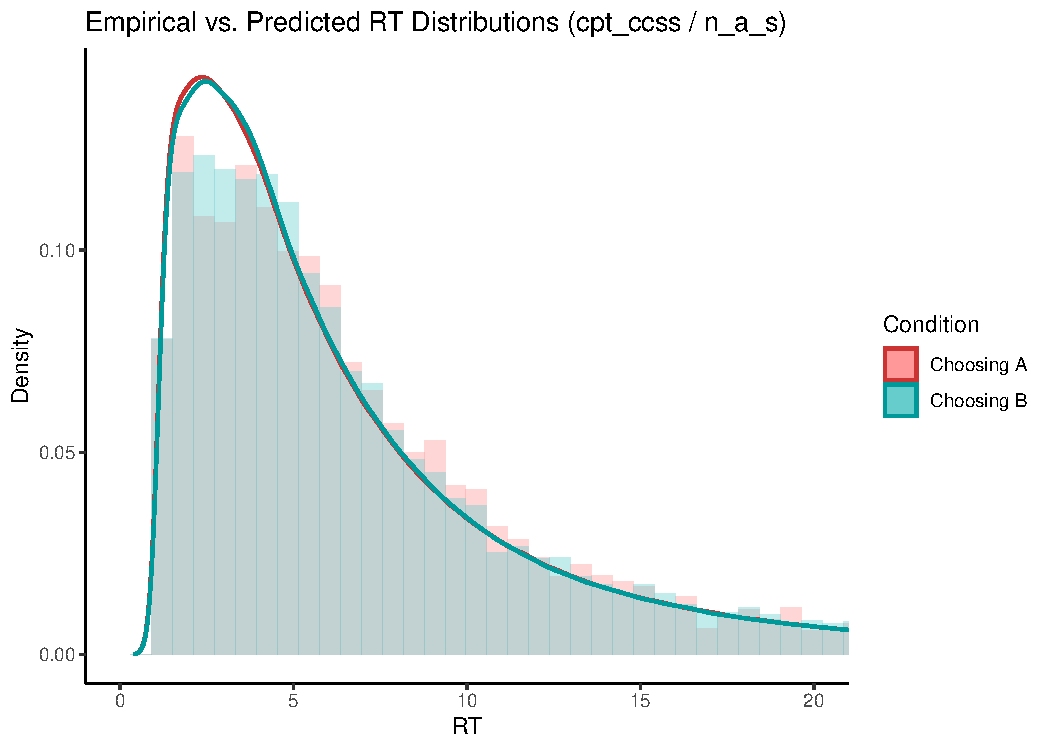
\includegraphics[width=\linewidth]{figures/ppc_rtdist_cpt_ccss_study2.pdf}\\[-2pt]{\footnotesize (d) CPT --- CCSS condition}\end{minipage}

\vspace{2pt}
\raggedright\textit{Note.} Conventions as in Figure~\ref{fig:rtdist_study1}.
\end{figure}

\begin{figure}[!htbp]
\caption{Empirical vs.\ Posterior-Predicted RT Distributions for the Best-Fitting Models, Study~3}
\label{fig:rtdist_study3}
\centering
\begin{minipage}{0.49\textwidth}\centering
  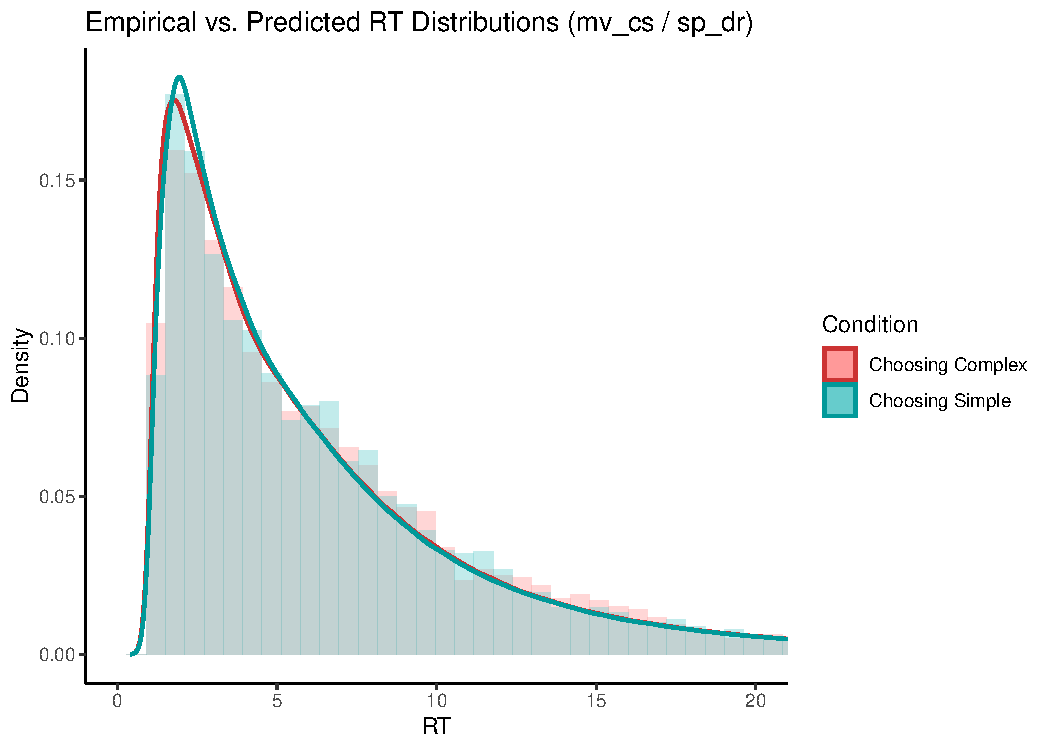
\includegraphics[width=\linewidth]{figures/ppc_rtdist_mv_cs_study3.pdf}\\[-2pt]{\footnotesize (a) MVS --- CS condition}\end{minipage}\hfill
\begin{minipage}{0.49\textwidth}\centering
  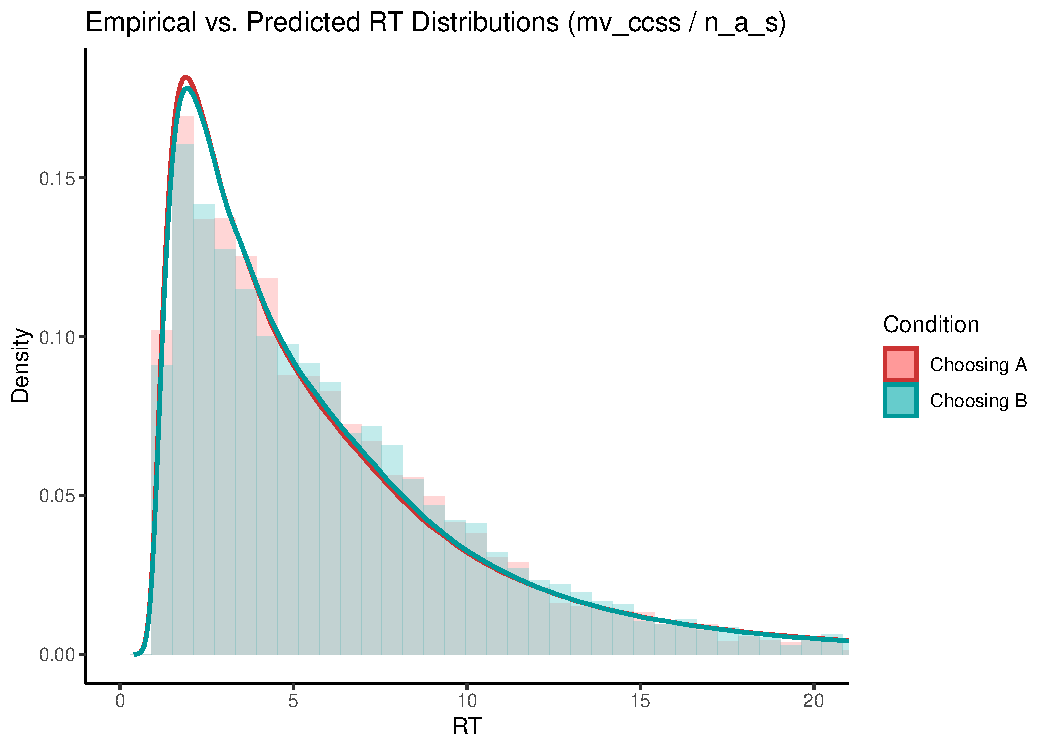
\includegraphics[width=\linewidth]{figures/ppc_rtdist_mv_ccss_study3.pdf}\\[-2pt]{\footnotesize (b) MVS --- CCSS condition}\end{minipage}

\vspace{4pt}
\begin{minipage}{0.49\textwidth}\centering
  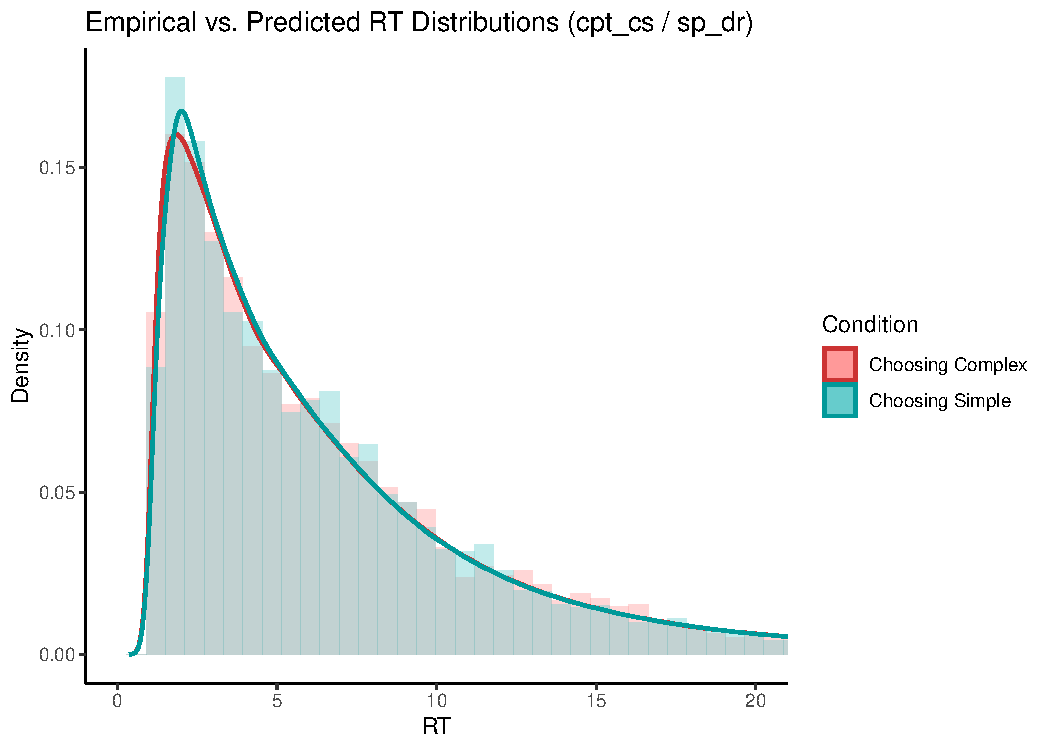
\includegraphics[width=\linewidth]{figures/ppc_rtdist_cpt_cs_study3.pdf}\\[-2pt]{\footnotesize (c) CPT --- CS condition}\end{minipage}\hfill
\begin{minipage}{0.49\textwidth}\centering
  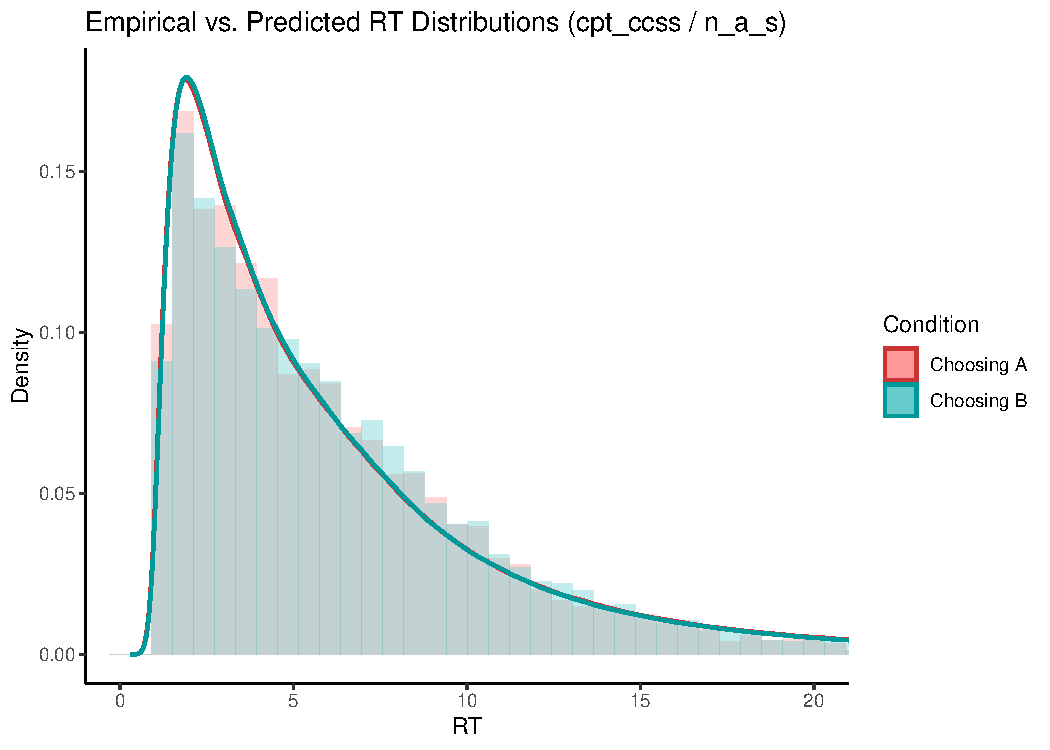
\includegraphics[width=\linewidth]{figures/ppc_rtdist_cpt_ccss_study3.pdf}\\[-2pt]{\footnotesize (d) CPT --- CCSS condition}\end{minipage}

\vspace{2pt}
\raggedright\textit{Note.} Conventions as in Figure~\ref{fig:rtdist_study1}.
\end{figure}

\FloatBarrier

%% ============================================================================
\section{Race-Model Diagnostic: Per-Accumulator Noise Identifiability}
\label{sec:rdm_diagnostic}
%% ============================================================================

A central claim of our framework is that complexity lowers the rate of evidence accumulation---it makes the evidence for a complex option accumulate more slowly and less reliably. In the main-text DDM this degradation is summarised by the drift-scaling parameter $\Delta_\theta$. One interesting question is whether we can test this hypothesis more directly, by asking whether the \emph{rate of evidence accumulation} differs between the two available options. The DDM cannot separate these because it contains a single diffusive-noise parameter by construction \parencite{donkin_overconstraint_2009,stevenson_emc2_2026}. The racing diffusion model \parencite[RDM;][]{tillman_sequential_2020} makes the distinction estimable: it represents the decision as two independent accumulators---one per response---each with its own drift rate, threshold, and \emph{within-trial noise} parameter $s$. Our hypothesis then carries a concrete signature---greater accumulation noise for the complex than for the simple option, that is, a ratio $s_{\text{complex}} / s_{\text{simple}} > 1$---and the RDM provides a direct test of it.

\subsection{RDM Specification}

The per-option noise hypothesis is implemented in the RDM through the per-accumulator within-trial noise parameter $s$. Using the \texttt{EMC2} package \parencite{stevenson_emc2_2026}, we specified, on the CS/SC trials of Study 2 ($N = 138$; median 87 trials per participant): drift rate $v \sim 0 + l_R + l_R : (\text{EVD} + \text{SDD} + \text{SkewD})$; within-trial noise $s \sim 0 + l_R$ with $s_{\text{simple}} = 1$ anchored for identifiability \parencite{donkin_overconstraint_2009}, so that $s_{\text{complex}} / s_{\text{simple}}$ is the free noise contrast that operationalises the hypothesis; response threshold $B \sim 0 + l_R$; a shared start-point range $A \sim 1$; and non-decision time $t_0 \sim 1$. Priors on all log-scale parameters were weakly informative and centred on psychologically plausible values. Models were fitted with four independent particle Metropolis-within-Gibbs chains on the sciCORE cluster (16 CPUs).

\subsection{Identifiability and Parameter Recovery}

Whether $s_{\text{complex}} / s_{\text{simple}}$ can be estimated reliably in this design is not obvious. Per-accumulator parameters in evidence-accumulation models are known to be poorly identified when one response type is rare \parencite{luken_parameter_2024}: threshold and accumulation-rate parameters become strongly correlated and trade off to produce nearly identical predictions. We therefore assessed identifiability directly with a simulation-based parameter recovery \parencite[following][]{baribault_troubleshooting_2025}. We generated 30 synthetic datasets of 50 simulated participants each, drawing \emph{all} 13 group-level parameters independently from plausible ranges---not anchored to the empirical fit---and drawing per-participant parameters around those group means; each simulated participant was assigned a real Study-2 participant's CS/SC trial sequence, so recovery was evaluated against the true stimulus structure. A light guard resampled any simulated participant with a degenerate ($<2\%$ or $>98\%$) complex-choice rate. Each dataset was refitted with the identical EMC2 design and priors, and true and recovered values were compared for every parameter (Figure~\ref{fig:rdm_recovery}).

The result is a clear three-tier pattern. The model's \emph{core} parameters recovered well: the drift-rate value slopes (on EVD, SDD, and SkewD, for both accumulators), the simple-option drift intercept and threshold, and the non-decision time all reached Pearson correlations between true and recovered participant-level values of $r = .91$--$.96$, with 93--97\% credible-interval coverage. The parameters specific to the \emph{complex-option} accumulator recovered less well: the complex drift intercept ($r = .80$), the complex-option threshold ($r = .69$), and---critically---the within-trial noise ratio $s_{\text{complex}} / s_{\text{simple}}$ ($r = .63$), whose group-level intervals were badly calibrated (43\% coverage). This asymmetry, in which each complex-accumulator parameter recovers worse than its simple-option counterpart, is the expected consequence of the complex option being chosen less often, so its accumulator is less constrained by the data. The shared start-point range $A$ was essentially unrecovered ($r = .49$), as is typical for this parameter. The sampler tells the same story: across the 30 datasets the poorly-identified parameters ($A$, $s_{\text{complex}}$, $B_{\text{complex}}$) drove elevated $\hat{R}$ (17 of 30 datasets exceeded $1.05$) and low effective sample sizes (minimum bulk ESS below 400 in every dataset), whereas the drift and non-decision-time parameters mixed normally.

The within-trial noise ratio $s_{\text{complex}} / s_{\text{simple}}$ is therefore only \emph{weakly and imprecisely} recovered, even under balanced simulated data. On the real Study-2 data identifiability is worse still: 22 of 138 participants (16\%) chose the complex option fewer than 15 times, exactly the rare-response regime that undermines per-accumulator estimation \parencite{luken_parameter_2024}.

\begin{figure}[!htbp]
\caption{Participant-Level Parameter Recovery for the Hierarchical RDM}
\label{fig:rdm_recovery}
\begin{center}
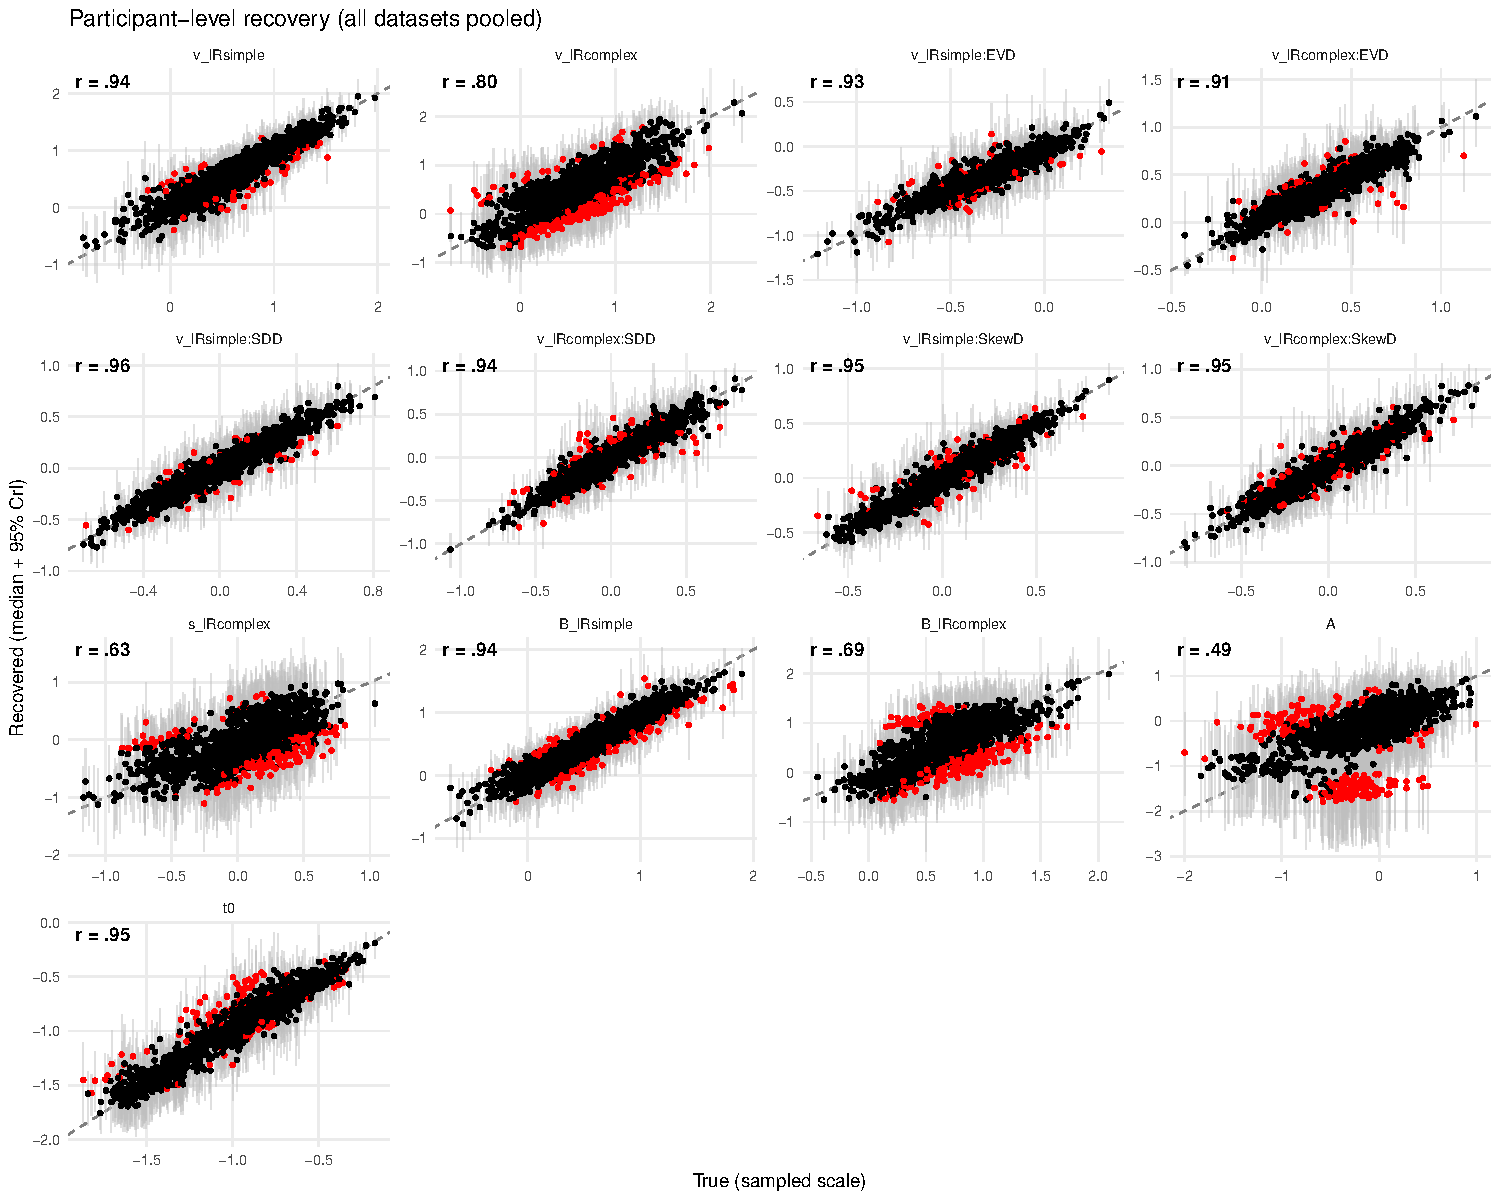
\includegraphics[width=\textwidth,height=0.82\textheight,keepaspectratio]{figures/rdm_recovery_individual.pdf}
\end{center}
\raggedright\textit{Note.} True (x-axis) versus recovered posterior-median (y-axis) values for each of the 13 group-level RDM parameters, pooled across 30 simulated datasets of 50 participants each, on the sampled (log/additive) scale. Vertical bars are 95\% credible intervals; red points mark intervals that exclude the true value; the dashed diagonal is perfect recovery. Each panel is annotated with its Pearson $r$. 
\end{figure}


%% ============================================================================
\section{Exploratory Analyses: Cognitive Ability and Complexity-Related Phenomena}
\label{sec:ca_correlations}
%% ============================================================================

The preregistration outlined three exploratory hypotheses linking individual differences in cognitive ability to complexity-related choice phenomena. We report all three tests transparently and then add a post-hoc mediation analysis motivated by the unexpected directional pattern observed for the second hypothesis.

\subsection{Preregistered Hypotheses}

\noindent\textit{Hypothesis 4.2.1.} Higher cognitive ability is associated with a higher proportion of complex-option choices on CS/SC trials (Spearman correlation expected to be positive).

\noindent\textit{Hypothesis 4.2.2.} Higher cognitive ability is associated with smaller condition-induced shifts in the latent signal-to-noise parameter (Spearman correlation between $\Delta_\theta$ and cognitive ability expected to be negative, on the rationale that participants with higher cognitive ability should be less affected by complexity in their latent choice consistency).

\noindent\textit{Hypothesis 4.2.3.} Larger condition-induced shifts in the latent signal-to-noise parameter are associated with lower proportions of complex-option choices on CS/SC trials (Spearman correlation between $\Delta_\theta$ and complex-choice rate expected to be negative, reasoning that participants more affected by complexity in their latent consistency should also avoid complex options more often when given a choice).

\subsection{Measures}

\textit{Behavioural complex-choice rate.} For each participant, we computed the proportion of trials on which the complex option was chosen on CS/SC trials (after excluding catch trials), with the complex option defined by the trial-level mapping between option-side and complexity level.

\textit{Latent signal-to-noise shift ($\Delta_\theta$).} For each participant, we extracted the posterior mean of $\Delta_\theta$ from the variant of the CCSS model in which only the signal-to-noise ratio varied by condition (model $n$). This is the simplest specification in which $\Delta_\theta$ is identified, so the estimate is not confounded with shifts in other condition-varying parameters. We did this separately for the CPT-based family (\texttt{cpt\_ccss\_7o} for Study 1 and \texttt{cpt\_ccss} for Studies 2 and 3) and for the MVS family (\texttt{mv\_ccss}) to verify that conclusions did not depend on the choice of value representation.

\textit{Cognitive ability.} The composite cognitive-ability score is the average of accuracy on the Berlin Numeracy Test (BNT) and a second numeracy assessment (HMT) administered as part of the cognitive battery. We use this composite (the variable \texttt{ca\_average} in the data files) without further transformation.

\subsection{Statistical Procedure}

All correlations are reported as Spearman's rank-order coefficient $\rho_s$, accompanied by two-sided $p$ values from the asymptotic Spearman test and 95\% confidence intervals derived from 5{,}000 nonparametric bootstrap resamples. Sample sizes reflect the intersection of participants present in the behavioural, cognitive-ability, and model-fit data sources for each study (Study 1: $N = 137$; Study 2: $N = 138$; Study 3: $N = 132$).

\subsection{Results}

\subsubsection{Hypothesis 4.2.1: Complex-Choice Rate and Cognitive Ability}

The expected positive association between cognitive ability and the proportion of complex-option choices was observed in Study 1, $\rho_s = .23$, $p = .008$, 95\% CI $[.05, .39]$, but did not replicate in Study 2, $\rho_s = .09$, $p = .298$, 95\% CI $[-.09, .26]$, or Study 3, $\rho_s = .04$, $p = .645$, 95\% CI $[-.13, .20]$. The preregistered prediction is therefore supported only under the number-of-outcomes manipulation of complexity used in Study 1 and does not generalise to the arithmetic-expression manipulation of Study 2 or the compound-probability manipulation of Study 3.

\subsubsection{Hypothesis 4.2.2: Latent Signal-to-Noise Shift and Cognitive Ability}

Across all three studies and both value representations, $\Delta_\theta$ correlated negatively with cognitive ability (Table~\ref{tab:ca_dtheta}). The bootstrap 95\% confidence interval excluded zero in four of the six study-by-family combinations.

\begin{table}[!htbp]
\centering
\begin{threeparttable}
\caption{Spearman Correlations Between $\Delta_\theta$ and Cognitive Ability}
\label{tab:ca_dtheta}
\begin{tabular}{llrrr}
\toprule
\textbf{Study} & \textbf{Family} & $\rho_s$ & $p$ & \textbf{95\% CI} \\
\midrule
Study 1 ($N = 137$) & CPT  & $-.16$ & $.057$  & $[-.33, +.01]$ \\
                    & MVS  & $-.17$ & $.046$  & $[-.33, -.00]$ \\
Study 2 ($N = 138$) & CPT  & $-.23$ & $.006$  & $[-.39, -.06]$ \\
                    & MVS  & $-.28$ & $< .001$ & $[-.43, -.12]$ \\
Study 3 ($N = 132$) & CPT  & $-.19$ & $.034$  & $[-.35, -.01]$ \\
                    & MVS  & $-.14$ & $.105$  & $[-.31, +.04]$ \\
\bottomrule
\end{tabular}
\begin{tablenotes}[flushleft]
\small
\item \textit{Note.} $\rho_s$ = Spearman rank-order correlation. CIs are bootstrap percentile intervals from 5{,}000 resamples. $\Delta_\theta$ was extracted from the $n$ variant of the CCSS family of each model (CPT or MVS).
\end{tablenotes}
\end{threeparttable}
\end{table}

The literal direction of the correlation matches the preregistered expectation (negative $\rho_s$). However, the substantive interpretation is reversed. Across all three studies, $\Delta_\theta$ is negative for nearly all participants ($96\%$, $95\%$, and $92\%$ in Studies 1, 2, and 3, respectively), reflecting the population-level reduction in signal-to-noise under complexity. A more negative $\rho_s$ between $\Delta_\theta$ and cognitive ability therefore implies that participants with higher cognitive ability show \textit{larger} (more negative) condition-induced consistency drops, not smaller ones. In other words, the data are consistent with the literal sign of the prediction but contradict its underlying rationale---that high-cognitive-ability participants are less affected by complexity. The pattern replicates across two structurally different complexity manipulations and across both value representations, ruling out a study- or model-specific artefact. The next subsection presents a post-hoc mediation analysis aimed at understanding this directional reversal.

\subsubsection{Hypothesis 4.2.3: Latent Signal-to-Noise Shift and Complex-Choice Rate}

The expected negative association between $\Delta_\theta$ and the proportion of complex-option choices was not observed (Table~\ref{tab:dtheta_pcomplex}). Across all three studies and both value representations, the signed $\rho_s$ values clustered near zero, and no bootstrap 95\% confidence interval excluded zero. The latent within-condition consistency-loss parameter and the between-condition complex-choice rate appear to tap independent individual differences in this dataset.

\begin{table}[!htbp]
\centering
\begin{threeparttable}
\caption{Spearman Correlations Between $\Delta_\theta$ and Complex-Choice Rate}
\label{tab:dtheta_pcomplex}
\begin{tabular}{llrrr}
\toprule
\textbf{Study} & \textbf{Family} & $\rho_s$ & $p$ & \textbf{95\% CI} \\
\midrule
Study 1 ($N = 137$) & CPT  & $+.01$ & $.917$ & $[-.15, +.17]$ \\
                    & MVS  & $-.01$ & $.897$ & $[-.17, +.15]$ \\
Study 2 ($N = 138$) & CPT  & $-.04$ & $.643$ & $[-.22, +.14]$ \\
                    & MVS  & $-.06$ & $.525$ & $[-.23, +.12]$ \\
Study 3 ($N = 132$) & CPT  & $+.03$ & $.755$ & $[-.15, +.20]$ \\
                    & MVS  & $+.04$ & $.692$ & $[-.14, +.20]$ \\
\bottomrule
\end{tabular}
\begin{tablenotes}[flushleft]
\small
\item \textit{Note.} $\rho_s$ = Spearman rank-order correlation. CIs are bootstrap percentile intervals from 5{,}000 resamples. $\Delta_\theta$ was extracted from the $n$ variant of the CCSS family of each model.
\end{tablenotes}
\end{threeparttable}
\end{table}

\subsection{Post-Hoc Mediation: A Floor-Effect Account}

The reversal for Hypothesis 4.2.2 has a simple explanation: cognitive ability may predict the \emph{baseline} signal-to-noise rate in the simple (SS) condition rather than the size of the complexity-induced shift. On the latent scale this baseline is $\theta_{SS} = \theta_{\text{raw}} - \Delta_\theta$ (from $v = (\theta + \Delta_\theta \cdot \text{con}) \cdot (\text{value terms})$, with $\text{con} \in \{-1, +1\}$). If higher-ability participants start from a higher $\theta_{SS}$, they have more ``room to fall'' under complexity and so show a larger negative $\Delta_\theta$---in which case the apparent $\Delta_\theta$--ability correlation would merely reflect baseline differences.

Using each participant's posterior-mean $\theta_{\text{raw}}$ and $\Delta_\theta$ (from the $n$ variant), we tested this with Spearman correlations and a rank-based partial correlation (residualising $\Delta_\theta$ and cognitive ability on $\theta_{SS}$; bootstrap 95\% CIs, 5{,}000 resamples), separately for the CPT and MVS families. The account holds in all six study-by-family combinations (Table~\ref{tab:floor_effect}): cognitive ability was positively associated with $\theta_{SS}$ ($\rho_s = +.29$ to $+.37$), $\Delta_\theta$ was negatively associated with $\theta_{SS}$ ($\rho_s = -.19$ to $-.83$), and partialling out $\theta_{SS}$ reduced the $\Delta_\theta$--ability correlation to between $-.11$ and $+.08$, with every bootstrap CI including zero. The apparent association between cognitive ability and the complexity-induced signal-to-noise reduction is thus fully explained by baseline consistency.

\begin{table}[!htbp]
\centering
\begin{threeparttable}
\caption{Floor-Effect Mediation: Per-Study Spearman Correlations}
\label{tab:floor_effect}
\begin{tabular}{llrrrr}
\toprule
\textbf{Study} & \textbf{Family} & $\theta_{SS} \sim$ CA & $\Delta_\theta \sim \theta_{SS}$ & $\Delta_\theta \sim$ CA & Partial \\
\midrule
Study 1 & CPT & $+.35^{***}$ & $-.26^{**}$  & $-.16$       & $-.08$ \\
        & MVS & $+.36^{***}$ & $-.19^{*}$   & $-.17^{*}$   & $-.11$ \\
Study 2 & CPT & $+.32^{***}$ & $-.76^{***}$ & $-.23^{**}$  & $+.02$ \\
        & MVS & $+.37^{***}$ & $-.83^{***}$ & $-.28^{***}$ & $-.04$ \\
Study 3 & CPT & $+.29^{***}$ & $-.76^{***}$ & $-.19^{*}$   & $+.05$ \\
        & MVS & $+.31^{***}$ & $-.65^{***}$ & $-.14$       & $+.08$ \\
\bottomrule
\end{tabular}
\begin{tablenotes}[flushleft]
\small
\item \textit{Note.} CA = cognitive ability score. ``Partial'' is the Spearman partial correlation between $\Delta_\theta$ and CA after rank-residualisation against $\theta_{SS}$. Bootstrap 95\% confidence intervals (not shown) for the partial correlation include zero in every cell. \\
\textsuperscript{$*$}$p < .05$. \textsuperscript{$**$}$p < .01$. \textsuperscript{$***$}$p < .001$.
\end{tablenotes}
\end{threeparttable}
\end{table}

\subsection{Interpretation}

Three findings warrant emphasis. First, the preregistered behavioural prediction (Hypothesis 4.2.1) was supported in Study 1 only and did not generalise across complexity manipulations. Second, the preregistered prediction relating $\Delta_\theta$ to cognitive ability (Hypothesis 4.2.2) was confirmed in its literal sign, but its substantive rationale was reversed: participants with higher cognitive ability showed \textit{larger}, not smaller, condition-induced reductions in signal-to-noise. Third, this directional reversal is fully accounted for by a baseline-consistency mechanism. Higher-cognitive-ability participants enter the SS condition with greater choice consistency, and the magnitude of the complexity-induced reduction scales with this baseline. Once baseline consistency is partialled out, cognitive ability does not further predict the complexity-induced shift in any of the three studies.

The data therefore support a refined account: \textit{cognitive ability is a robust predictor of baseline (SS-condition) choice consistency, but it does not predict the differential sensitivity of consistency to complexity over and above this baseline-level relationship}. This refinement is methodologically important because it shows that an apparent cognitive-ability-by-complexity interaction can arise from a purely baseline-level cognitive-ability effect when the dependent measure is a difference score. We note one caveat: in Studies 2 and 3, the rank correlation between $\theta_{SS}$ and $\Delta_\theta$ exceeds $|\rho_s| = .65$, and part of this coupling may reflect joint posterior structure imposed by the hierarchical Bayesian fit (e.g., shared shrinkage and prior-induced correlations) rather than a purely psychological mechanism. The mediation interpretation does not require a clean separation between these sources, however, because the partial correlation between $\Delta_\theta$ and cognitive ability is the appropriate test in either case.

The third preregistered hypothesis (Hypothesis 4.2.3) was not supported in any study. This null is consistent with the broader pattern observed in the main text: the latent within-condition consistency parameter and the directional preference for simpler options reflect partially distinct individual differences.

%% ============================================================================
\section{Software and Reproducibility}
\label{sec:software}
%% ============================================================================

All model fitting and analyses were conducted on the sciCORE high-performance computing cluster at the University of Basel, using AMD EPYC 7742 64-Core processors. The full analysis pipeline---including Stan model source files, R scripts for data preprocessing, model fitting, parameter recovery, and model comparison---is available at [repository URL].

\begin{table}[!htbp]
\centering
\begin{threeparttable}
\caption{Software Versions Used in All Analyses}
\label{tab:software}
\begin{tabularx}{\textwidth}{lX}
\toprule
\textbf{Component} & \textbf{Version} \\
\midrule
R & 4.4.2 \\
CmdStan & 2.38.0 \\
\texttt{cmdstanr} & 0.8.1 \\
\texttt{posterior} & 1.6.0 \\
\texttt{loo} & 2.8.0 \\
\texttt{rtdists} (recovery simulations) & 0.11-5 \\
Operating system (cluster) & Ubuntu Linux \\
CPU & AMD EPYC 7742 64-Core \\
\bottomrule
\end{tabularx}
\begin{tablenotes}[flushleft]
\small
\item \textit{Note.} Analyses were run on the sciCORE high-performance computing cluster at the University of Basel.
\end{tablenotes}
\end{threeparttable}
\end{table}

% Ensure the loo R package appears in the bibliography (mentioned in Table S5
% as a software dependency but not cited inline).
\nocite{vehtari_loo_2024}

\clearpage
\printbibliography

\end{document}
